\documentclass[a4paper, twoside]{report}

%% Language and font encodings
\usepackage[english]{babel}
\usepackage[utf8x]{inputenc}
\usepackage[T1]{fontenc}

%% Sets page size and margins
\usepackage[a4paper,top=3cm,bottom=2cm,left=3cm,right=3cm,marginparwidth=1.75cm]{geometry}

%% Useful packages
\usepackage{amsmath}
\usepackage{graphicx}
\usepackage{float}
\usepackage{needspace}
\usepackage{mdframed}
\usepackage{etoolbox}
\usepackage{booktabs}
\usepackage{tabularx}
\usepackage{array}
\usepackage{longtable}
\usepackage[colorinlistoftodos]{todonotes}
\usepackage[colorlinks=true, allcolors=blue]{hyperref}
\usepackage{subcaption}
\usepackage{tikz}
\usetikzlibrary{arrows.meta, positioning, shapes.geometric}
\usepackage{listings}
\lstset{
  basicstyle=\ttfamily\small,
  breaklines=true,
  frame=single,
  columns=fullflexible,
  keepspaces=true,
  aboveskip=\baselineskip,
  belowskip=\baselineskip,
}
%% Keep each listing block on one page (no split across page breaks).
\surroundwithmdframed[
  nobreak=true,
  linewidth=0pt,
  innerleftmargin=0pt,
  innerrightmargin=0pt,
  innertopmargin=0pt,
  innerbottommargin=0pt,
  leftmargin=0pt,
  rightmargin=0pt,
  skipabove=\baselineskip,
  skipbelow=\baselineskip,
]{lstlisting}
%% If less than ~45\% of the page remains, start the listing on a fresh page.
\BeforeBeginEnvironment{lstlisting}{\Needspace{0.45\textheight}}
%% For bibliography
\setcounter{secnumdepth}{3}

\title{Scenario-Driven Evaluation and Testing of Tool-Using LLM Agents}
\author{Ruthvik Konduru}
% Update supervisor and other title stuff in title/title.tex

\begin{document}
\input{title/title.tex}

% \begin{abstract}
% Your abstract goes here
% \end{abstract}

% \renewcommand{\abstractname}{Acknowledgements}
% \begin{abstract}
% Thanks mum!
% \end{abstract}

\tableofcontents
\listoffigures
\listoftables

% \section{Objectives}
% \section{Challenges}
% \section{Contributions}

\chapter{Introduction}
\label{chap:introduction}

\section{Motivation}

Large Language Models (LLMs) have moved from being standalone text generators to being embedded inside increasingly complex software systems. Early progress in large-scale language modelling showed that Transformer-based models could perform a wide range of tasks from natural language prompts alone \cite{vaswani2017attention,brown2020language}, and instruction tuning made these models more useful as general-purpose assistants that follow user intent \cite{ouyang2022training}. More recently, LLMs have been used as agents: systems that plan over multiple steps, call tools, retrieve information, interact with users, and modify external state. Approaches such as ReAct demonstrated the value of combining reasoning with action \cite{yao2023react}, while work such as Toolformer and API-Bank showed the growing importance of external tool use in language model systems \cite{schick2023toolformer,li2023apibank}. This shift has changed the central reliability question. It is no longer sufficient to ask whether a model can produce a plausible final answer; we must ask whether an agent followed the right process, called the right tools, respected domain rules, and left the external system in a correct state.

For teams deploying agents in consequential settings, that question is not academic. A support agent that sounds polite but skips authentication, calls the wrong account tool, or leaves a ticket in an invalid state can cause real harm even when the final reply reads well. Building dependable agents therefore requires a workflow closer to software engineering than to prompt tuning alone: define the behaviour you expect, run the agent against those expectations, inspect what failed, fix the agent or policy, and repeat until the constraints hold. Without tooling that supports that loop, teams cannot move from ``it worked once in the playground'' to justified confidence that an agent will behave correctly under repeated, varied interaction.

Existing evaluation approaches only partly support that workflow. Traditional benchmarks and LLM-as-a-judge methods such as HELM, G-Eval, and MT-Bench are valuable for comparing models on isolated inputs and final outputs \cite{liang2022holistic,liu2023geval,zheng2023judging}, but they hide failures that live in tool traces and application state: a final answer can look reasonable while the agent skipped a required step or changed state incorrectly. Recent agent benchmarks such as AgentBench, WebArena, $\tau$-bench, and AppWorld have made trace- and state-aware evaluation more visible \cite{liu2023agentbench,zhou2023webarena,yao2024taubench,trivedi2024appworld}, yet they are fixed leaderboards rather than reusable infrastructure for a domain team writing its own behavioural contracts. Practical libraries and observability tools help developers run checks and inspect traces, but they still make it awkward to express a full multi-turn scenario (with output, tool, and state checks together) and to get precise diagnostics when something fails. Chapter~\ref{chap:related-work} analyses those limitations in detail.

This project addresses that need with \emph{agent-spec-kit}: a framework for scenario-driven evaluation of LLM agents. Its central bet is that reliability comes from \emph{declarative} behavioural specifications that a team can read, run, and iterate on. A scenario reads like a conversation script: user messages, checks on the agent's reply and tool use after each turn, and optional state oracles, all in one place. When an assertion fails, the framework reports which expectation broke and where in the trace it applied, so developers can fix the agent quickly rather than reconstruct the episode from a raw trace or aggregate score. The approach draws on software-testing ideas such as test oracles, repeated trials, and failure simplification \cite{claessen2000quickcheck,barr2015oracle,zeller2002simplifying,ribeiro2020checklist}. The goal is to make desired agent behaviour explicit, runnable, and inspectable, so failures are specified before they happen, discovered systematically, and preserved as regression tests for the next change.

\section{Contributions}

This project makes the following high-level contributions.

\begin{itemize}
    \item \textbf{A declarative, co-located scenario language for agent behaviour.} The project provides a way to define agent evaluations as executable scenarios rather than as isolated prompt--output pairs scattered across datasets, graders, and runner config. A scenario reads as a conversation script: user messages, checks on the agent's reply and tool use after each turn, optional environment steps, and repeat counts live in one place. That makes behavioural contracts easier for teammates to read, review, and change as product rules evolve.

    \item \textbf{Support for evaluating multiple surfaces of agent behaviour.} Instead of treating the final natural-language response as the only evaluation target, the framework supports checks over the user-facing output, intermediate tool interactions, and resulting application state. This reflects the observation from recent agent benchmarks that correctness in tool-using systems depends on trajectories and state changes, not only final answers \cite{yao2024taubench,trivedi2024appworld,lu2024toolsandbox}.

    \item \textbf{Assertion-local diagnostics and a testing-oriented failure workflow.} The project brings ideas from software testing into LLM agent evaluation, including repeated trials, generative variation of scenarios, simplification of failing cases, and extraction of regression tests. When an assertion fails, the framework reports which expectation broke, where in the trace it applied, and structured expected versus actual detail, so developers can fix the agent or policy without reconstructing the episode from a raw trace or aggregate score alone.

    \item \textbf{A practical evaluation workflow for domain-specific agents.} The framework is designed around the spec--run--inspect--fix loop that teams need when building agents with rules, tools, and stateful side effects. The contribution is not a new benchmark alone, but reusable infrastructure for constructing domain-specific evaluations where success criteria are explicit, rerunnable, and comparable across experiments.

    \item \textbf{An empirical evaluation of the framework on agent tasks.} The project evaluates the framework by applying it to realistic tool-using agent scenarios and analysing the kinds of failures that are found. The evaluation focuses not only on aggregate pass rates, but also on whether the framework helps expose distinct failure modes and turn them into reproducible regression cases.
\end{itemize}

Overall, this project contributes a developer-facing evaluation framework for LLM agents. Its central claim is that reliable agent development requires more than scalar benchmark scores or LLM-judged final answers: it requires declarative behavioural specs that a team can read, run repeatedly, and debug precisely when they fail.


\chapter{Background}

\section{Large Language Models and the Transformer Architecture}

Modern large language models (LLMs) are built on the Transformer architecture, which introduced the self-attention mechanism as a replacement for recurrent or convolutional networks in sequence modeling. In the seminal “Attention is All You Need” paper \cite{vaswani2023attentionneed}, the authors showed that a Transformer using only attention could achieve state-of-the-art results in machine translation, with faster training and better parallelism. The attention mechanism allows a model to weigh the relevance of different words in the input when producing each part of the output, effectively letting the model “focus” on important context. Multiple attention “heads” capture different relationships in parallel, enabling rich representations of language. This architecture is the backbone of today’s LLMs and is largely responsible for their ability to capture long-range dependencies and complex patterns in text.
\newline

\begin{figure}[h]
\centering
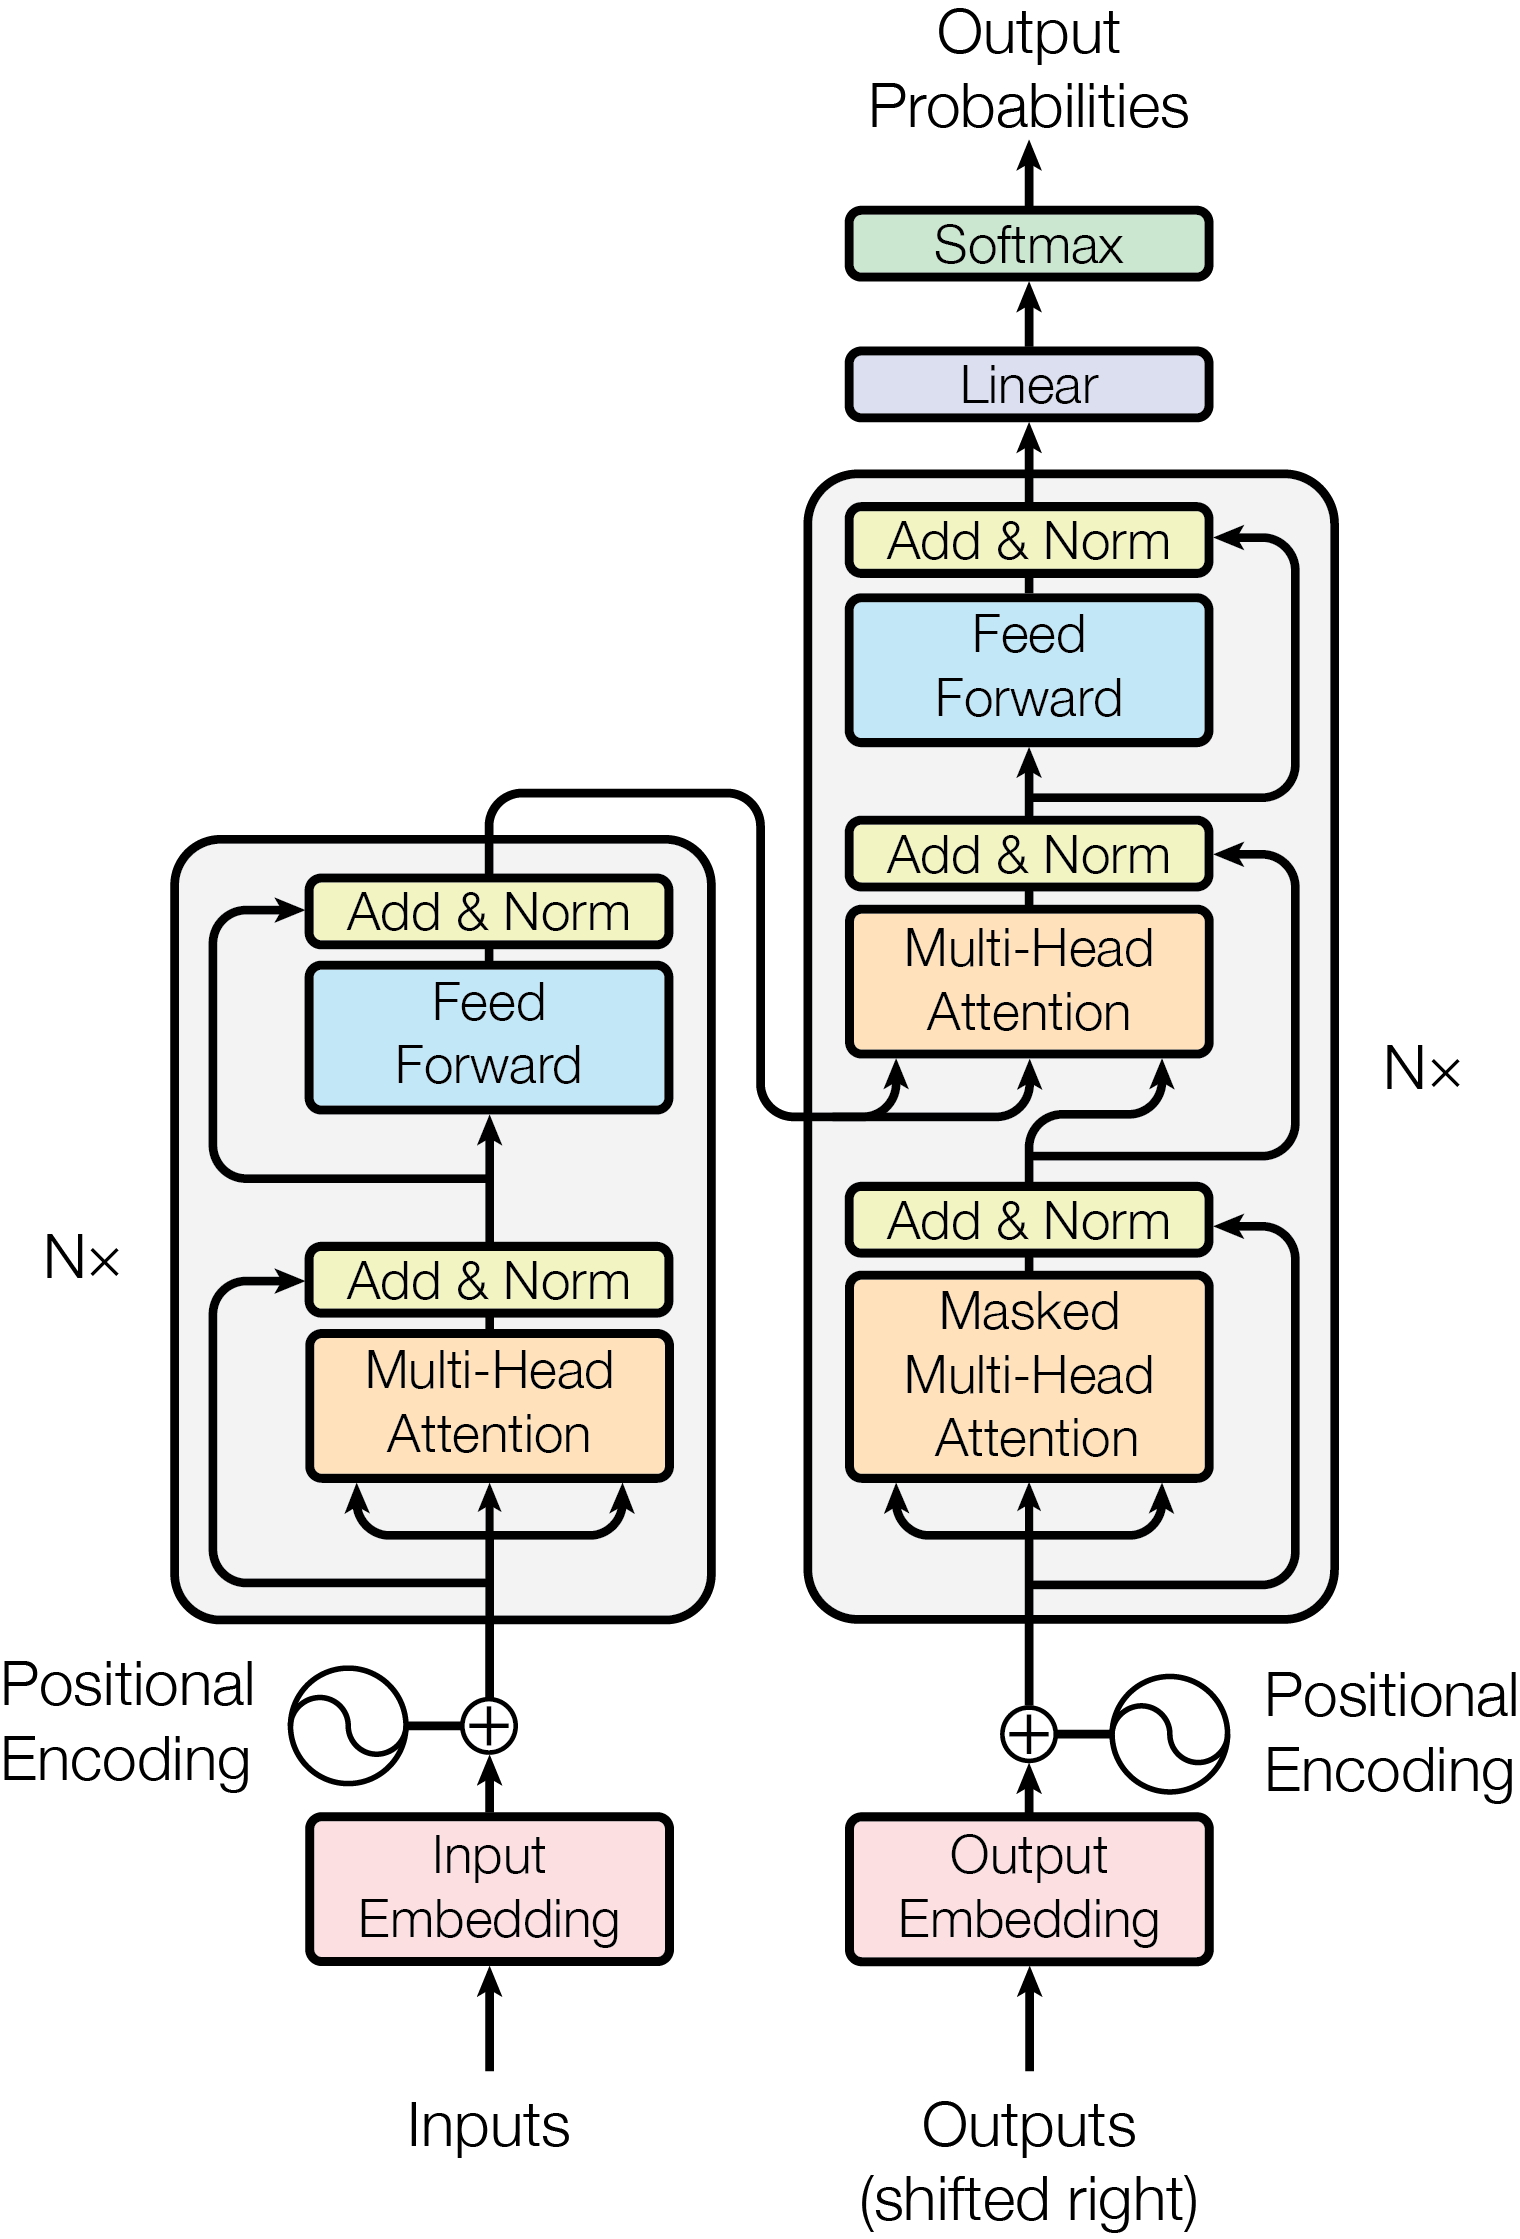
\includegraphics[width=0.35\textwidth]{figures/transformer.png}
\caption{The Transformer - model architecture \cite{vaswani2023attentionneed}}
\end{figure}

Crucially, LLMs are trained on massive corpora of text via self-supervised learning (predicting the next word or masked words). This scaling of model size and data has led to emergent capabilities. Notably, GPT-3 (175 billion parameters) demonstrated that simply making models larger unlocks in-context learning abilities: GPT-3 could perform many tasks without gradient updates or fine-tuning, given only a prompt with a few examples or an instruction. In their paper “Language Models are Few-Shot Learners” \cite{brown2020languagemodelsfewshotlearners}, Brown et al. showed that GPT-3, when prompted with a task description and a few input-output examples (known as few-shot), achieved strong results on translation, question-answering, and other NLP tasks. The same model can solve diverse tasks zero-shot or few-shot by understanding the task from its prompt. Performance on many benchmarks approached that of models explicitly fine-tuned on those tasks. This revealed that very large transformers inherently learn to follow instructions and examples given in the prompt, essentially “programming” the model through natural language.
\newline

\begin{figure}[h]
\centering
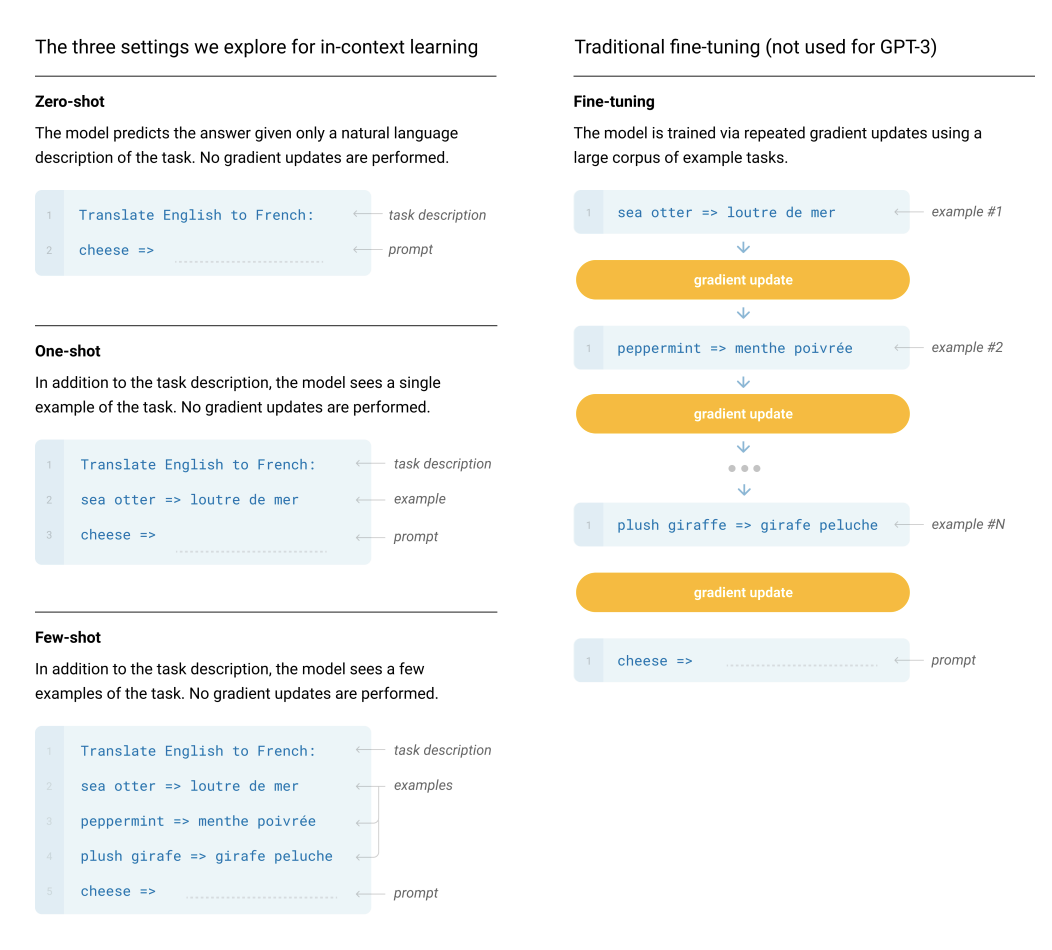
\includegraphics[width=0.85\textwidth]{figures/few_shot_example.png}
\caption{Zero-shot, one-shot and few-shot, contrasted with traditional fine-tuning \cite{brown2020languagemodelsfewshotlearners}}
\label{few-shot}
\end{figure}

At the same time, the authors noted limitations, some tasks still stumped the model and it sometimes produced incorrect or nonsensical outputs (due to data biases or reasoning limits). These failure modes foreshadow issues like hallucination that we discuss later. Nonetheless, the Transformer based LLM paradigm of pretraining on broad data, then prompting the model for downstream tasks, has become the foundation for current AI systems.

\section{Prompting Techniques for LLMs}

Because LLMs can understand and follow prompts, a new field of “prompt engineering” has emerged to get the best performance from them. A variety of prompting techniques have been developed to improve accuracy, reasoning, and reliability.
\newline

In zero-shot prompting, we just give the model an instruction or question and ask for an answer. Large models like GPT-3 were surprisingly capable in the zero-shot setting \cite{brown2020languagemodelsfewshotlearners}, but performance often improves if we provide more guidance.
\newline

In few-shot prompting (in-context learning) as shown in figure \ref{few-shot}, the prompt includes a handful of examples of the task with inputs and desired outputs, before the actual query. This “demonstration” primes the model on the task format and desired behavior. The GPT-3 work showed that with enough parameters, models can rapidly generalise from just a few examples provided in the prompt \cite{brown2020languagemodelsfewshotlearners}. For instance, given two or three example translations (English–French), GPT-3 can translate a new sentence without any fine-tuning. Few-shot prompts essentially perform on-the-fly conditioning of the model, and the order and choice of examples can affect performance. Researchers found that prompt design details (e.g. example ordering) can be important, a phenomenon dubbed prompt order sensitivity \cite{lu2022fantasticallyorderedpromptsthem}. Best practices (such as “fantastically ordered prompts” have been proposed to choose and order demonstrations to maximise accuracy.
\newline

In instruction prompting, rather than examples, we can give a clear natural language instruction. Instruction-tuned models (like InstructGPT \cite{ouyang2022traininglanguagemodelsfollow} or ChatGPT) have been further trained to better follow explicit instructions. For instance, a prompt like: “Summarise the following text in one paragraph.” will guide the model’s behavior. The success of instruction tuning shows that models can internalise a general notion of following user commands.
\newline

In chain-of-thought (CoT) prompting, one major advance for reasoning tasks is to prompt the model to produce a step-by-step reasoning trace before giving the final answer \cite{wei2023chainofthoughtpromptingelicitsreasoning}. In chain-of-thought prompting, we include in the prompt an example of a question followed by a human-like reasoning process (a series of steps or thoughts) concluding with the answer. When the model is prompted to “Let’s think step by step,” it will output a chain of logical steps and then an answer. Wei et al. \cite{wei2023chainofthoughtpromptingelicitsreasoning} showed this dramatically improves performance on arithmetic word problems, commonsense reasoning, and other tasks that require multi-step thinking. The improvement is so substantial that chain-of-thought was identified as an emergent ability of sufficiently large models, smaller models cannot do it well, but models with tens of billions of parameters suddenly can. For example, a 540B model given 8 examples of chain-of-thought reasoning achieved state-of-the-art on the GSM8K \cite{cobbe2021trainingverifierssolvemath} math word problem benchmark, outperforming even some fine-tuned approaches \cite{wei2023chainofthoughtpromptingelicitsreasoning}. The model effectively “reasons out loud,” reducing errors in tasks like math where keeping track of partial results is crucial.
\newline

\begin{figure}[h]
\centering
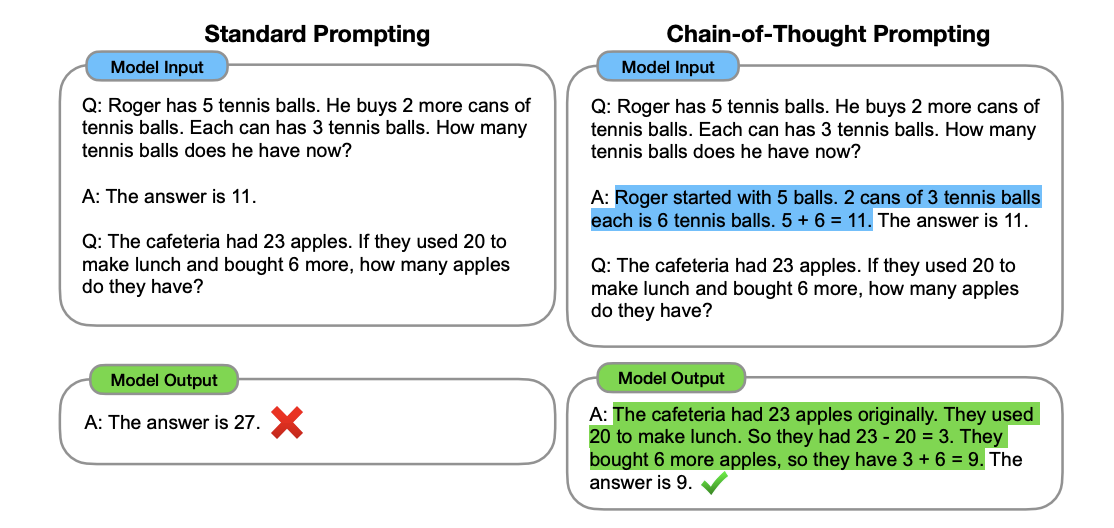
\includegraphics[width=0.85\textwidth]{figures/chain-of-thought.png}
\caption{Chain of thought prompting \cite{wei2023chainofthoughtpromptingelicitsreasoning}}
\end{figure}

An intriguing variant is Zero-Shot CoT, proposed by Kojima et al. \cite{kojima2023largelanguagemodelszeroshot}, simply appending a phrase like “Let’s think step by step.” to the prompt often triggers the model to produce a chain of reasoning, even without any examples. This trick enabled strong performance on reasoning benchmarks, for instance, accuracy on a math dataset (MultiArith \cite{roy2016solvinggeneralarithmeticword}) jumped from 17.7\% to 78.7\% by adding that prompt phrase for an InstructGPT model \cite{kojima2023largelanguagemodelszeroshot}. This demonstrates that models have latent reasoning abilities that the right prompt can unlock.
\newline

In self-consistency decoding, after obtaining a chain-of-thought, one can further boost reliability by using self-consistency. Instead of taking the model’s first answer, we sample the model multiple times (each time it may produce a different reasoning chain and answer). We then aggregate the answers (e.g. by majority vote). Wang et al. \cite{wang2023selfconsistencyimproveschainthought} found that this method significantly improved accuracy on reasoning tasks, the most consistent answer across multiple sampled reasoning paths is usually correct. For example, with GSM8K math problems, self-consistency improved accuracy by nearly 18\% versus a single chain-of-thought \cite{wang2023selfconsistencyimproveschainthought}. The intuition is that complex problems often have multiple ways to reach the solution, and if many independent reasoning attempts converge on the same answer, it’s likely correct. Self-consistency also reduces sensitivity to any one flawed chain-of-thought or particular phrasing of the prompt.
\newline

Scratchpad prompting \cite{nye2021workscratchpadsintermediatecomputation} is similar to CoT, encouraging the model to work out intermediate calculations explicitly. We also have prompts that induce the model to verify or reflect on its answer (e.g. generate a solution, then generate a “check” or critique). These approaches aim to reduce mistakes by leveraging the model’s own capabilities in a multi step prompt. As an example, prompting a model to “reflect on whether the answer could be wrong and why” can catch obvious errors and have it correct itself in a second attempt.
\newline

Overall, these techniques show that how you prompt an LLM can be as important as what task you ask, the prompt shapes the model’s behavior profoundly. As a result, prompt design has evolved from simple Q\&A examples to sophisticated strategies that elicit reasoning and self checking. These methods drive the idea that the prompt itself can teach or guide the model without changing the model’s weights. This forms the basis for building more complex LLM-driven systems.

\section{LLM Agents and Pipeline Architectures}

While a well-crafted single prompt can often get impressive results, there are limits to what an LLM can do in one go, especially for complex, knowledge-intensive, or interactive tasks. This has motivated the development of LLM based agents and multi-step pipeline architectures that go beyond a single prompt and response. These architectures integrate the LLM with additional tools or break problems into smaller sub-tasks, often yielding greater accuracy and flexibility. We discuss two prominent architectures: ReAct \cite{yao2023reactsynergizingreasoningacting} and Retrieval Augmented Generation \cite{yang2018hotpotqadatasetdiverseexplainable}, as examples of LLM agents and retrieval-based pipelines, respectively.
\newline

\subsection{ReAct}

ReAct (Reasoning + Acting) is a framework that combines the strengths of chain-of-thought reasoning with the ability to take actions (such as calling external tools or querying a database) in an interleaved manner. In a ReAct agent, the LLM’s output is structured to alternate between reasoning traces (thinking steps in natural language) and action commands that the agent executes in an environment or via an API. For example, faced with a question, the model might reason “I should look up this person’s birthdate” (reasoning) and then output an action like \texttt{SEARCH("Person Name birthdate")}. The agent executes the search, retrieves results, and feeds them back to the model, which continues reasoning with the new information, and so on. By explicitly prompting the model to both “think” and “act,” ReAct creates a closed loop where the model can gather evidence and update its plan. This combination of reasoning and acting enables more powerful problem-solving.
\newline

Critically, the reasoning trace helps the model decide which action to take next and how to handle the tool outputs, while the tools ground the model’s knowledge and reduce hallucinations. Yao et al. demonstrated ReAct on tasks like factual question answering (with a Wikipedia search API) and interactive decision-making (in a text-based game environment) \cite{yao2023reactsynergizingreasoningacting}. On knowledge tasks such as HotpotQA \cite{yang2018hotpotqadatasetdiverseexplainable} (multi-hop QA) and FEVER \cite{thorne2018feverlargescaledatasetfact} (fact verification), ReAct was able to reduce hallucination and error propagation by retrieving relevant facts before final answer generation \cite{yao2023reactsynergizingreasoningacting}. The model’s chain-of-thought ensures that it uses the retrieved information effectively and provides a rationale, resulting in more interpretable and trustworthy outputs compared to a black-box prompt that directly answers. For instance, rather than guessing an answer from its parametric memory (and possibly getting it wrong), a ReAct agent will explicitly say “According to the article I found, the person was born in 1980”, tying the answer to an external source.
\newline

In interactive environments (like an ALFWorld household task \cite{shridhar2021alfworldaligningtextembodied} or the WebShop online shopping task \cite{yao2023webshopscalablerealworldweb}), ReAct significantly outperformed traditional reinforcement learning agents, despite using only a few in-context examples for prompting \cite{yao2023reactsynergizingreasoningacting}. The ability to maintain a high-level plan in the reasoning while executing step-by-step actions is key. Overall, ReAct exemplifies why one would build a more complex LLM-based agent: a plain prompt might hallucinate missing facts or be unable to interact with external systems, whereas an agent can dynamically query tools, navigate environments, and correct itself using intermediate results.

\begin{figure}[h]
\centering
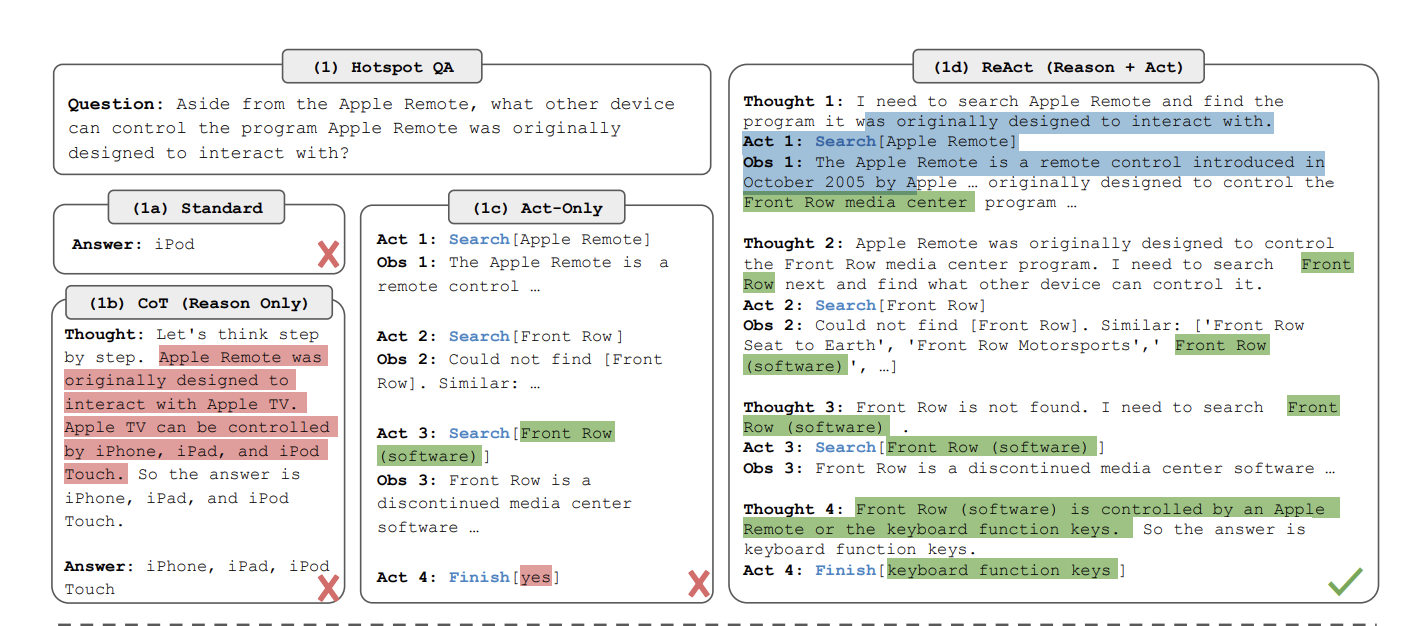
\includegraphics[width=0.95\textwidth]{figures/react.png}
\caption{(1) Comparison of 4 prompting methods, (a) Standard, (b) Chain-of-thought (CoT, Reason Only), (c) Act-only, and (d) ReAct (Reason+Act), solving a HotpotQA  question. \cite{yao2023reactsynergizingreasoningacting}}
\end{figure}

\subsection{Retrieval-Augmented Generation}

Retrieval-Augmented Generation (RAG) \cite{lewis2021retrievalaugmentedgenerationknowledgeintensivenlp} is another powerful architecture that combines an LLM with a dedicated retrieval system, forming a pipeline that first fetches relevant context from a knowledge source and then generates the answer. In the original RAG framework, a large Transformer-based generative model is augmented with a non-parametric memory (e.g. a vector-indexed Wikipedia) that it can query. When asked a question, the system uses a retriever to pull, say, the top-$k$ text passages related to the query. Those passages are then provided to the LLM as additional context in the prompt, and the model is tasked with producing an answer that integrates that information.
\newline

The key benefit is that the LLM is no longer limited to the facts stored in its fixed weights, it has an external knowledge base it can utilise. Lewis et al. showed that a RAG model fine-tuned on open-domain QA achieved state-of-the-art results on several benchmarks, outperforming models that relied only on parametric memory \cite{lewis2021retrievalaugmentedgenerationknowledgeintensivenlp}. Moreover, the outputs were judged to be more specific and factually accurate than those from a comparable model without retrieval. By design, RAG provides a traceable origin of information since the model’s answer can be linked to the retrieved sources, which is important for trust and verification. RAG based pipelines have become popular in industry for building domain-specific assistants: e.g., a legal assistant LLM can be connected to an internal document repository so that it always cites the relevant policy or law rather than hallucinating. The retrieval component can be updated independently (e.g. add new documents) without retraining the language model, making maintenance easier. Beyond QA, retrieval is used in tasks like long-form summarisation (retrieve related references), dialogue (recall facts mentioned earlier or user profile info), etc. Essentially, whenever current knowledge or reference to source material is needed, a RAG architecture is beneficial. It’s an example of a more complex pipeline that solves a problem a raw LLM cannot. No matter how big the model, it might not know about events from after its training cutoff, but a retrieval module can fetch up-to-date info for it to use.
\newline

Both ReAct and RAG illustrate why developers compose LLMs into larger tool-using pipelines or agents. A plain LLM prompt is a single-shot attempt at the task, which may fall short if the task requires multiple steps of reasoning, external knowledge, or interacting with an environment. By adding structure around the LLM, we can overcome these limitations. An LLM agent can decompose a task (explicitly thinking step by step, using sub-results) and invoke external tools (e.g. search engines, calculators, databases, APIs) to handle subtasks that the LLM isn’t reliable at. This often yields better results than a monolithic prompt. For example, even an LLM can make arithmetic mistakes on large numbers if prompted directly, but an agent that calls a calculator will get it exactly right. Similarly, rather than expecting the LLM to internally know every fact (which leads to hallucination when it doesn’t), a RAG pipeline compels it to base answers on retrieved documents. There is also a modularity benefit: one can upgrade the retriever or add new tools without changing the core LLM.
\newline

This added complexity, however, comes with new challenges, especially in ensuring these multi-step systems are reliable. We next examine common failure modes that can occur in LLM agents and pipelines.

\section{Common Failure Modes of LLMs and Agents}

Despite their impressive capabilities, LLMs are far from infallible. They exhibit several failure modes - tendencies to produce incorrect or undesired outputs, which can be exacerbated in complex agent or pipeline settings. Understanding these failure modes helps motivate techniques (like prompt optimisation and human feedback) to mitigate them.
\newline

One well-known issue is hallucination. An LLM is said to hallucinate when it fabricates information that is not grounded in reality or provided sources. For example, an LLM might confidently state a wrong date or cite a non-existent article. Hallucinations often arise in open-ended generation when the model’s training data lead it to produce a reasonable sounding answer that is false. This is especially problematic in factual tasks. With a standard prompt, the model might not admit ignorance and instead “guess” an answer.
\newline

In multi-step agents, hallucination can manifest as the agent hallucinating intermediate steps or tool outputs that haven’t actually been verified. For instance, a ReAct agent might generate a reasoning step saying “(Search result shows X)”, when in fact no such result was found, effectively hallucinating the content of a tool’s output. The ReAct paper \cite{yao2023reactsynergizingreasoningacting} explicitly noted that a pure chain-of-thought approach without tool use was prone to error propagation. The model might assume a false fact in its reasoning and then stick with it to the final answer. By introducing real tool results, ReAct aimed to break that cycle. However, if the agent’s prompt isn’t carefully designed, it might ignore the tool output or misuse it, still leading to incorrect answers. Retrieval-augmented generation systems also face a related failure mode, if the retriever pulls irrelevant passages or if the model doesn’t properly incorporate the evidence, the final answer can be wrong or only loosely related to the query. In other words, having a tool or context doesn’t guarantee it’s used correctly. Thus the prompts guiding the agent must enforce faithfulness (e.g. “use the retrieved document to justify your answer”). If the prompt is weak, the model might revert to its parametric knowledge and hallucinate an answer that conflicts with the retrieved data.
\newline

Another failure mode is inability to follow instructions or format when the prompt is suboptimal. LLMs can be very sensitive to prompt phrasing. A slight ambiguity or a missing detail in instructions can lead the model astray. For example, if an agent’s prompt doesn’t explicitly tell the model when to stop reasoning, the model might go into an endless loop of tool calls. Or if the prompt for a multi-step task is under-specified, the model might skip necessary steps. It has also been observed that even changing the order of few-shot examples or wording of a single instruction can substantially alter performance \cite{lu2022fantasticallyorderedpromptsthem}. As a result, pipelines and agents often require extensive manual prompt trial-and-error to become reliable. This brittleness is a key motivator for prompt optimisation methods later discussed.
\newline

In complex multi-turn interactions, context handling can fail. A chatbot agent might forget important details given earlier (context window limits) or confuse information from different turns. An agent might also inadvertently reveal private tool outputs or system instructions if the prompt is not well constructed to prevent that (a kind of prompt leakage), and in production systems these risks can be exploited via prompt injection \cite{liu2024automaticuniversalpromptinjection,reddy2025echoleakrealworldzeroclickprompt,zheng2023judgingllmasajudgemtbenchchatbot}. Once again these failure modes trace back to prompt content and how the agent is directed to manage memory and confidentiality.
\newline

It’s worth noting that evaluating some of these failures itself is non-trivial. Determining whether an LLM’s answer is correct can be as hard as the answering the original question. If the question requires expert knowledge, an automated system may not easily verify the answer’s correctness without that same knowledge. This is why many LLM answers need human review, and why automatic evaluation often struggles (we delve into evaluation frameworks next). An implication is that building a reliable agent often becomes an iterative process, identify a failure (model gave a wrong or nonsensical result), then adjust the prompt or pipeline to address it. Many failures in agents can be traced back to prompt inadequacies e.g., the prompt didn’t stress the required format, or didn’t remind the model to use the tool output, or contained phrasing that triggered an unintended behavior. This back and forth is slow, frustrating and is another motivator for systematic prompt optimisation. If we can automatically find prompt tweaks that eliminate or reduce these failure modes, we can greatly improve the overall system performance.
\newline

These failure modes motivate the need for systematic evaluation, how can we reliably distinguish correct, well-reasoned outputs from flawed ones, and whether this assessment can be automated. This leads to a discussion of existing frameworks for evaluating LLM outputs and identifying “good” versus “bad” responses.

\section{Existing Evaluation Frameworks for LLM Outputs}

Evaluating the performance of LLMs in complex, open-ended tasks is a challenging task. Traditional NLP metrics like BLEU or ROUGE often fall short for generative models, because a model’s output might be valid even if it doesn’t overlap with a reference text. Furthermore, for many tasks there is no single “ground truth” answer. As a result, a number of evaluation frameworks and techniques have been proposed to assess LLM outputs. Two recent frameworks gaining traction are DeepEval \cite{deepevalQuickIntroduction} and Ragas \cite{ragasRagas}, which we discuss as examples. We also highlight the limitations of automated metrics and LLM-based evaluators, which motivate incorporating human judgment.
\newline

\subsection{DeepEval}

DeepEval is an open-source framework that treats evaluation like writing test cases for an LLM. Instead of relying only on coarse metrics, it allows users to define evaluation criteria in plain language and uses LLMs themselves to grade outputs against those criteria. One of DeepEval’s metrics is G-Eval \cite{liu2023gevalnlgevaluationusing}, a “LLM-as-a-judge” approach. The idea is that you provide a description of what a good output looks like (for example: “The answer should correctly solve the problem and be stated clearly in one sentence.”). DeepEval then uses a LLM to compare the output to the expected qualities or to a reference solution, and produce a score. Essentially, an LLM is used as an automatic evaluator, following the rubric you wrote in natural language.
\newline

\begin{figure}[h]
\centering
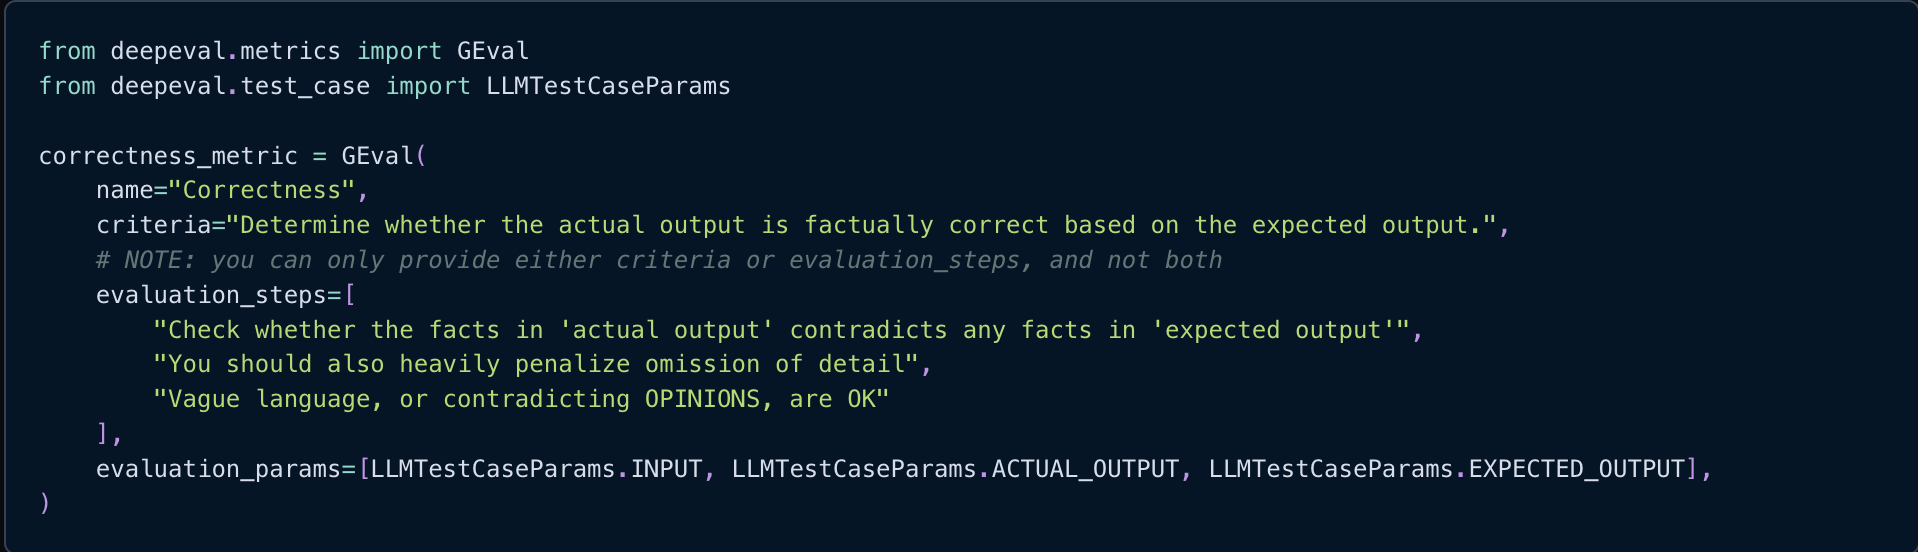
\includegraphics[width=0.95\textwidth]{figures/geval_instantiation.png}
\caption{Instantiating a G-Eval metric using the DeepEval Python library \cite{deepevalQuickIntroduction}}
\end{figure}

This approach can be applied to many dimensions of quality: correctness, coherence, relevance, style, safety, etc. For instance, DeepEval’s G-Eval has been used in various scenarios: checking answer correctness (e.g. “Was the model’s answer actually right?”), coherence in multi-turn conversations (did the response logically follow the conversation), tonality (does the output have the desired tone, say formal vs casual), and adherence to knowledge (for a RAG system, “Did the model only use the retrieved documents and not introduce outside info?”). These evaluations run automatically and can be integrated into CI/CD pipelines for continuous monitoring of an LLM application. The benefit of LLM-based evaluators is that they can handle the complexity of natural language outputs better than rigid metrics. For example, they can notice if an answer is factually wrong or off-topic, which a simple string overlap metric would miss. In practice, this means teams can rapidly test changes to prompts or models by seeing how the LLM’s outputs score on a suite of G-Eval tests.


\subsection{RAGAS}

Let's consider a RAG system, evaluating it has multiple facets \cite{es2025ragasautomatedevaluationretrieval}:
\begin{enumerate}
    \item Did the retrieval component identify passages that are relevant to the query?
    \item Did the language model faithfully ground its response in the retrieved passages, rather than ignoring them or hallucinating unsupported content?
    \item Does the answer directly address the question in
an appropriate way
\end{enumerate}
A single metric can’t capture all these, so Ragas provides a suite of metrics to probe each aspect \cite{es2025ragasautomatedevaluationretrieval,ragasRagas}. For example, Ragas includes metrics like \emph{Context Recall} and \emph{Context Precision}, which measure whether the content of the answer is supported by the retrieved context. Additionally, there are Relevance metrics to see if the retrieved text was actually relevant to the query (assessing the retriever’s quality) \cite{es2025ragasautomatedevaluationretrieval,ragasRagas}.
\newline

Rather than describing the full RAGAS metric suite, we illustrate the underlying evaluation methodology by detailing two representative metrics \emph{Faithfulness} and \emph{Answer Relevance}. These descriptions closely follow the original paper \cite{es2025ragasautomatedevaluationretrieval}:

\subsubsection{Faithfulness}
\label{subsubsec:faithfulness}

In the RAGAS framework, an answer $a_s(q)$ is said to be \emph{faithful} to the context $c(q)$ if the claims made in the answer can actually be inferred from the context. To estimate faithfulness, RAGAS first uses an LLM to extract a set of atomic statements $S(a_s(q))$ from the answer. The aim of this step is to decompose longer sentences into shorter and more focused assertions.

The following prompt is used for statement extraction:\footnote{To help clarify the task, a demonstration is included as part of the prompt in the original paper. This demonstration is not explicitly shown in the listing of prompts here.}

\begin{quote}
\small
\textbf{Given a question and answer, create one or more statements from each sentence in the given answer.} \\
question: [question] \\
answer: [answer]
\end{quote}

For each statement $s_i \in S(a_s(q))$, RAGAS determines whether $s_i$ can be inferred from the context $c(q)$ using a verification function $v(s_i, c(q))$. This verification step is carried out using the following prompt:

\begin{quote}
\small
\textbf{Consider the given context and following statements, then determine whether they are supported by the information present in the context. Provide a brief explanation for each statement before arriving at the verdict (Yes/No). Provide a final verdict for each statement in order at the end in the given format. Do not deviate from the specified format.} \\
statement: [statement 1] \\
\ldots \\
statement: [statement n]
\end{quote}

The final faithfulness score $F$ is computed as:
\[
F = \frac{|V|}{|S|}
\]
where $|V|$ is the number of statements that were supported according to the LLM and $|S|$ is the total number of extracted statements.

\subsubsection{Answer Relevance}
\label{subsubsec:answer_relevance}

In RAGAS, an answer $a_s(q)$ is considered \emph{relevant} if it directly addresses the question in an appropriate way. This assessment does not take factual correctness into account; instead, it penalises answers that are incomplete or contain redundant information.

To estimate answer relevance, the framework prompts an LLM to generate $n$ potential questions $\{q_i\}_{i=1}^n$ based on the given answer $a_s(q)$, using the following prompt:

\begin{quote}
\small
\textbf{Generate a question for the given answer.} \\
answer: [answer]
\end{quote}

Embeddings are then obtained for the original question $q$ and each generated question $q_i$ using an embedding model. For each $q_i$, the similarity $\mathrm{sim}(q, q_i)$ is computed as the cosine similarity between the corresponding embeddings.

The answer relevance score $AR$ is computed as:
\[
AR = \frac{1}{n} \sum_{i=1}^{n} \mathrm{sim}(q, q_i)
\]

This metric evaluates how closely the generated answer aligns with the original question or instruction.
\newline

For tool-using agents, RAGAS even has metrics like \emph{Tool Call Accuracy} (did the agent choose the correct tool/action at each step) and \emph{Agent Goal Accuracy} (did the agent ultimately achieve the goal?) \cite{ragasRagas}. RAGAS can perform reference-free evaluation, meaning it doesn’t require a human-provided correct answer for each query \cite{es2025ragasautomatedevaluationretrieval}. This is practical because in many real applications (like search engines or chat assistants), collecting a gold answer for every possible query is challenging. Instead, RAGAS relies on heuristics and LLM-based judgments on the model’s behavior and usage of information. The creators argue this can speed up the evaluation cycle for LLM systems, letting developers quickly quantify changes in retrieval or prompting strategies \cite{es2025ragasautomatedevaluationretrieval}.
\newline

However, both frameworks suffer from a core limitation, an automated evaluator is only as reliable as its understanding of the task and context. LLM-based judges, while flexible, can misfire in specialised or subjective domains where nuanced domain knowledge or personalisation is essential. For instance, consider a financial analyst requesting insights tailored to their specific risk profile. Evaluating the quality of such an output requires understanding user intent, acceptable tradeoffs, and relevant financial heuristics that even strong LLMs typically lack. For example, an analyst may have a counterintuitive preference for healthcare companies with high debt ratios, based on a belief that such firms are undervalued during certain market cycles. A generic LLM judge, unaware of this subtle preference, might wrongly penalise an otherwise appropriate recommendation. To further reinforce this point, let's consider some RAGAS metrics \cite{es2025ragasautomatedevaluationretrieval}: \emph{faithfulness} (Section \ref{subsubsec:faithfulness}) is unsuitable because it only checks whether the answer is supported by the retrieved context, not whether it reflects the analyst’s unstated preference, while \emph{answer relevance} (Section \ref{subsubsec:answer_relevance}) is unsuitable because it assesses whether the question is addressed, not whether the answer aligns with the user’s true intent. One might attempt to encode this context and user intent into an LLM judge's prompt (as done in G-Eval \cite{liu2023gevalnlgevaluationusing}), but in practice, defining a comprehensive evaluation specification upfront is difficult, time-consuming, and error-prone, even for domain experts. And even if such a specification is written, there is no guarantee that the LLM judge will interpret or follow it consistently, particularly when the criteria are subtle or subjective. In many cases, it is far easier and more reliable to annotate specific outputs with targeted feedback than to author an abstract, general-purpose rubric. This highlights a key issue, existing evaluators often fall short because the evaluation task itself is underdefined and sensitive to details that are hard to capture automatically.
\newline

In addition, frameworks such as DeepEval and RAGAS, rely on scalar metrics to summarise output quality. These scores are useful for broad comparisons, but they flatten complex feedback into a single number that may obscure rather than reveal the model’s behaviour. For example, it can be unclear what practically distinguishes a score of 5 from a 6, or how to act on that feedback when refining prompts or tuning an agent. This lack of granularity and interpretability limits their usefulness during optimisation, where developers often need actionable signals e.g., which part of the output failed, why, and how to improve it. By collapsing diverse quality attributes (e.g., relevance, reasoning, tone) into a single figure, scalar metrics lose important structure in the evaluation signal, making them poorly suited for guiding iterative improvements.
\newline

In general, evaluating correctness or quality in open-ended tasks is sometimes as hard as generating the answer in the first place. If even humans might debate what a “good” answer is (common in subjective or creative tasks), an automated metric will be at best a rough guideline. Thus, these evaluation frameworks are useful tools; they can catch obvious mistakes or regressions and provide quantitative feedback, but they do not eliminate the need for nuanced human judgment. Automated eval metrics do not fully correlate with actual user satisfaction or task success for complex tasks. One approach is to use these frameworks for quick iteration, but ultimately involve human evaluators or end-user feedback to truly assess if the LLM system is performing well.
\newline

\section{Existing Prompt Optimisation Methods}

Given the impact prompt design has on LLM performance, a number of automated prompt optimization methods have been proposed in recent years. These techniques aim to find better prompts systematically, rather than relying on manual trial-and-error by a human engineer. Many such methods treat prompt improvement as an optimisation problem: define some objective function (e.g. any performance metric like those provided by DeepEval \cite{deepevalQuickIntroduction} or Ragas) \cite{ragasRagas} and then search the space of possible prompts to maximise that objective. Below, we review several notable approaches and discuss their strengths and limitations.
\newline

\subsection{Automatic Prompt Optimization (APO)}

Automatic Prompt Optimization (APO) is an approach proposed by Reid et al. \cite{pryzant2023automaticpromptoptimizationgradient} that takes inspiration from gradient descent to iteratively refine prompts. The key idea is to use a LLM to generate a sort of “pseudo-gradient” in natural language. APO starts with an initial prompt and a validation set of query-answer pairs. It then feeds batches of examples to the LLM with the current prompt and obtains the model’s outputs. By comparing these outputs to the ground-truth answers, APO has the LLM critique the prompt, producing what the authors call a “natural language gradient”, which is essentially suggestions on how to edit the prompt to fix errors. For example, the LLM might observe that “the instructions are vague about format; expected a yes/no answer but got free text”. APO then applies this feedback by modifying the prompt in the opposite direction of the “gradient” (hence the analogy to gradient descent). APO uses a beam search over possible edits and a bandit algorithm to choose which edits to accept, balancing exploration and exploitation. This process repeats for several iterations, continually improving the prompt based on model-generated feedback. In experiments, APO significantly improved prompt performance on various NLP tasks, e.g. yielding up to a 31\% gain over the initial prompt by rewriting vague instructions into more precise ones \cite{pryzant2023automaticpromptoptimizationgradient}. Intuitively, APO automates what a human might do (test the prompt on examples, see where it fails, tweak the wording) but does it at scale with the model’s help. A limitation is that APO assumes access to a set of training examples and an automatic way to measure error on those examples (it uses the known correct answers to generate the “gradient”). Thus, it needs a well-defined metric per example (e.g. was the answer right or wrong), which might not be available for all tasks.

\begin{figure}[h]
\centering
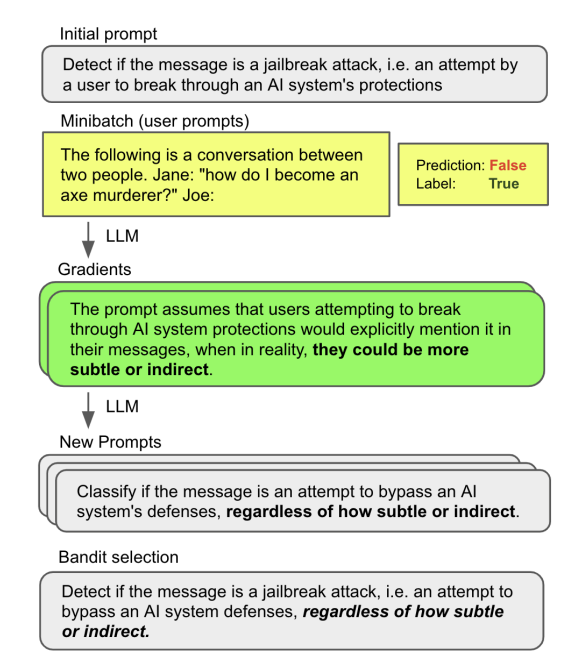
\includegraphics[width=0.5\textwidth]{figures/apo_overview.png}
\caption{APO overview \cite{pryzant2023automaticpromptoptimizationgradient}}
\end{figure}

\subsection{EvoPrompt}

EvoPrompt is a method that frames prompt optimisation as an evolutionary process \cite{guo2025evopromptconnectingllmsevolutionary}. EvoPrompt maintains a population of prompt candidates and iteratively evolves them using operators inspired by genetic algorithms (selection, crossover, mutation. An initial population could be, say, a few hand-written prompts or even random perturbations of a baseline prompt. Then in each generation, the following happens: the prompts are evaluated on a development set (again requiring some metric of performance), the top-performing prompts are “selected”, and less effective ones are discarded \cite{guo2025evopromptconnectingllmsevolutionary}. The selected prompts are then used to breed a new generation, EvoPrompt actually uses the LLM to generate new prompt variants by mutating or recombining the selected ones. For example, if two prompts in the population differ in wording, the LLM might produce a new prompt that combines phrases from both (crossover), or take a high-performing prompt and paraphrase one part of it (mutation). By repeating this, the prompt population ideally improves over time.
\newline

One challenge with natural language “genes” is maintaining prompt coherence, a random mutation could make the prompt ungrammatical or change its meaning entirely. EvoPrompt addresses this by leveraging the LLM’s own linguistic capabilities to ensure prompts remain well-formed. EvoPrompt, starting from scratch, was able to automatically discover prompts that outperform human-written prompts on a variety of tasks. For instance, on the BIG-Bench Hard suite (a set of challenging tasks) \cite{suzgun2022challengingbigbenchtaskschainofthought}, EvoPrompt’s optimised prompts achieved up to 25\% higher accuracy than the best human-designed prompts. This suggests that an evolutionary search, while computationally expensive, can stumble upon prompt formulations that humans might not think of. Again, the method assumes a way to score each prompt (so usually a supervised setting or at least something like “model got answer right/wrong”).

\subsection{OPRO}

OPRO (Optimization by Prompting) is an approach introduced by Yang et al. \cite{yang2024largelanguagemodelsoptimizers} that takes a meta-approach: use the LLM itself as an optimiser for arbitrary problems described in natural language. The “solutions” in this context are prompts. Concretely, one defines an optimisation task (e.g. “find a prompt that maximises accuracy on these math questions”) and encodes the current best solutions and their scores into a meta-prompt. The LLM then reads this meta-prompt and is asked to propose new candidate solutions (new prompts) \cite{yang2024largelanguagemodelsoptimizers}. After the LLM generates some new prompt ideas, those are evaluated on the task and the meta-prompt is updated with the new scores, then fed again to the LLM for the next iteration. This creates an optimisation loop entirely guided by the LLM’s generation capabilities. The model “imagines” improvements to the prompt given the history of what worked or not.
\newline

OPRO was demonstrated not only on prompt optimisation but also on classic optimisation problems (like traveling salesman) by describing the problem in words to the LLM \cite{yang2024largelanguagemodelsoptimizers}. For prompt optimisation specifically, OPRO yielded substantial gains. For example, it found better instruction prompts for a math word problem dataset (GSM8K) that improved accuracy by \textasciitilde 8\% over a strong human-written prompt. On the Big-Bench Hard tasks \cite{suzgun2022challengingbigbenchtaskschainofthought}, OPRO’s optimised prompts beat human prompts by up to 50\% in performance. These are big improvements, showing that an LLM, given a systematic procedure (the “meta-prompt”), can iteratively refine prompts in ways a person might not anticipate. One advantage of OPRO is its simplicity, it doesn’t require custom algorithms like beam search or evolutionary crossover; it basically prompts the model to do hill-climbing in the space of prompts. However, OPRO too needs a numerical reward to guide it (it uses the model’s performance on a validation set as the score). If the reward signal is noisy or absent, OPRO would struggle.

\begin{figure}[h]
\centering
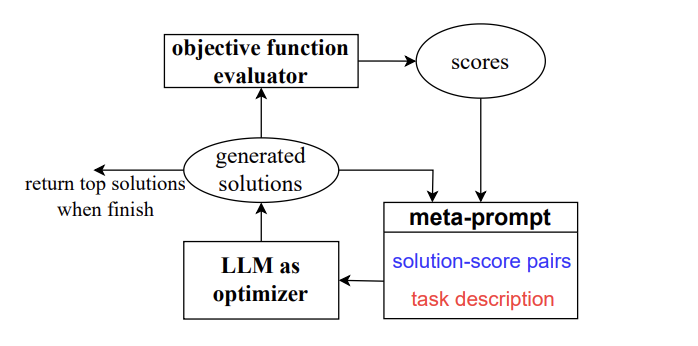
\includegraphics[width=0.6\textwidth]{figures/opro_overview.png}
\caption{OPRO overview \cite{yang2024largelanguagemodelsoptimizers}}
\end{figure}

\subsection{MIPRO}

MIPRO (Multiprompt Instruction Proposal Optimization) is a method designed for optimising multi-stage prompt pipelines (what they call LM Programs) where you may have several LLM calls in sequence \cite{opsahlong2024optimizinginstructionsdemonstrationsmultistage}. In a pipeline, each module has its own instructions and possibly few-shot examples. Jointly tuning all of them is complex because an improvement in one module’s prompt might hurt another module down the line. MIPRO addresses this by factorising the problem: it separately optimises the instructions for each module and the few-shot demonstrations, but uses a clever credit assignment to see which module’s changes actually improve the final output \cite{opsahlong2024optimizinginstructionsdemonstrationsmultistage}. One part of MIPRO’s approach is to generate candidate instructions that are grounded in the task context. For example, it can summarise the overall task and feed that into a prompt-proposal module so that new instructions stay relevant. Another part is a form of Bayesian Optimisation, MIPRO will try combinations of different module instructions and use a surrogate model to predict which combinations might yield the best final performance \cite{opsahlong2024optimizinginstructionsdemonstrationsmultistage}. It treats the entire pipeline’s prompts as tunable parameters, but without needing to observe intermediate module “gold” outputs (since often intermediate steps don’t have ground truth). Opsahl-Ong et al. reported that MIPRO delivered significant gains on complex pipelines, improving accuracy by up to 13\% over baseline on a set of multi-hop reasoning and decision tasks. Notably, MIPRO is capable of optimising both the instruction text and the selection of few-shot examples jointly. It does this by “bootstrapping” a pool of candidate demonstrations (by having the model generate some synthetic examples) and then picking an optimal subset and order of them for the prompt. This joint optimisation is important because an instruction and its examples interact, you need them to complement each other. MIPRO’s success shows that even very complex prompting scenarios can be systematically optimised, given a suitable evaluation metric. The limitation, like others, is the requirement of a scalar metric to optimise, MIPRO needs a function to tell it how well a given prompt configuration did (e.g. final answer accuracy) in order to guide the search. In purely subjective or open-ended tasks, defining such a metric is difficult.

\subsection{GEPA}

GEPA (Genetic-Pareto Optimization with Reflection) is a recent prompt optimisation algorithm. It deeply incorporates natural language feedback (reflection) into the optimisation loop \cite{agrawal2025gepareflectivepromptevolution}. The authors argue that conventional RL-style optimisation (which gives a single scalar reward like “score = 0.7”) is a very sparse learning signal for an LLM, whereas the model could learn much more effectively from rich descriptions of why an output was bad or how it could be improved \cite{agrawal2025gepareflectivepromptevolution}. GEPA combines ideas from genetic algorithms and LLM self-reflection. It generates a population of prompt variants and runs each through the task to see the outcomes. But instead of just getting a score for each, GEPA has the model reflect in natural language on each attempt: diagnosing errors, noticing patterns (“Prompt A tends to produce too verbose answers, prompt B made a factual error about X”). These reflections are then used to propose new prompt edits. Importantly, GEPA uses a Pareto frontier concept to retain a diverse set of best prompts (balancing trade-offs, e.g., one prompt might be very accurate but long, another concise but slightly less accurate). By analysing multiple top prompts, the model can combine “lessons” from them, for instance, “Include instruction Y from prompt 1 to avoid math errors, but also the concise style of prompt 2”. Over just a few iterations (even a few trials can yield big gains), GEPA manages to significantly improve prompts.
\newline

GEPA surpassed the earlier MIPRO optimiser by over 10\% on average across 4 tasks \cite{agrawal2025gepareflectivepromptevolution}. This validates the hypothesis that language can be a much richer learning medium for optimising language model behaviour. Essentially, GEPA is letting the model leverage its own understanding to guide prompt search. The model can tell us in words what is going wrong, which is far more informative than a numeric score. GEPA does still rely on an objective to ultimately select prompts (it uses the reflections to generate new candidates, but it still needs to test them and see which are better according to the task metric). However, by integrating qualitative feedback, it moves toward a scenario where even if you don’t have a perfect automatic metric, the model’s analysis can drive the optimisation.
\newline

Most of the above methods (except GEPA) largely reduce the feedback to a single scalar metric per prompt. They require either a labeled dataset or at least a way to automatically score outputs (e.g. compare to ground truth answers). In real-world tasks, obtaining such a metric can be the hardest part as discussed in the previous section. Often there is no automatic measure of correctness: for example, what’s the “score” of a chatbot’s response in a free-form conversation? You could attempt to train a reward model or use an LLM judge, but as we discussed, those are imperfect in domain-specific settings and can exhibit systematic biases \cite{wang2023largelanguagemodelsfair}. Lin et al. \cite{lin2024promptoptimizationhumanfeedback} explicitly acknowledge this: “previous works often require a numeric score to assess prompt quality…such a score is often infeasible and unreliable when a human user interacts with a black-box LLM”. This is a crucial point, if we don’t have a well-defined metric, methods like APO, EvoPrompt, and OPRO cannot directly be applied, or they may optimise for a proxy metric that doesn’t truly capture success. In addition these metrics provide a scalar reward, rather than fully using any nuanced feedback the model or user could provide. One can argue that rich natural language feedback could guide prompt optimisation more effectively. GEPA’s results support this, by using reflective feedback instead of just numeric rewards, it achieved larger improvements with fewer iterations \cite{agrawal2025gepareflectivepromptevolution}. This suggests that future optimisation could incorporate, for example, human-written feedback, not just preferences or scores. Finally, it’s worth noting that all these optimisation algorithms assume we have the ability to test prompts repeatedly using an LLM (often a large one), which in practice can be costly due to API usage or latency. So we can ask the question: how many prompt trials are worth doing to get an improved prompt? Methods like GEPA try to be sample-efficient (fewer trials by extracting more info per trial) \cite{agrawal2025gepareflectivepromptevolution}.
\newline

In summary, the field has produced a variety of prompt optimisation strategies. These have demonstrated substantial gains, validating that prompts are tunable artifacts. However, their common dependency on a scalar evaluation metric limits their direct applicability in many real-world settings where such metrics are absent or incomplete. This is a key motivation for integrating human feedback into the optimisation loop, as we discuss later. Before that, we consider existing software frameworks that aim to make prompt/agent optimisation more accessible.

\section{Existing Frameworks for Prompt/Agent Optimisation}

Thus far we’ve discussed algorithms for optimising prompts. In practice, a developer also needs tooling to apply these methods to their LLM application. The main framework in this area is DSPy (Stanford, 2024), which provides an end-to-end system for writing language model pipelines and optimising them \cite{khattab2023dspycompilingdeclarativelanguage}. We’ll use DSPy as a case study of existing frameworks, what they offer and where they might fall short in usability.
\newline

DSPy stands for “Declarative Structured Programming for LMs”, it lets developers define a pipeline of LM calls (an LM program) in a declarative way, and then automatically compiles and optimises that program \cite{khattab2023dspycompilingdeclarativelanguage}. You can think of it as analogous to TensorFlow or PyTorch but for prompting rather than neural network layers. In DSPy, you define modules with input/output fields (like function signatures but for prompts) and connect them into a graph (e.g. a retrieve module followed by a generate module in a RAG pipeline). Each module can have a parameterized prompt, meaning the instruction template and few-shot examples are treated as parameters to be learned/tuned. DSPy’s “compiler” can then apply built-in optimisation algorithms to those prompt parameters to maximise a user-specified metric. For example, you could declare that the final answer from the pipeline should be evaluated by accuracy against a test set, and DSPy will attempt to adjust the prompts of intermediate modules to improve that accuracy. Under the hood, it leverages methods like bootstrapping examples, OPRO, MIPRO, etc., but abstracts them away from the user. The user just writes their pipeline in a high-level way, and calls something like \texttt{dspy.optimise(pipeline, metric=...)}. DSPy will then perhaps generate demonstrations, try different instructions, and output an optimised set of prompts. In two case studies, the DSPy team showed that a few lines of DSPy code could express fairly sophisticated agents (for multi-hop QA, math reasoning, etc.) and after a few minutes of optimisation, the pipeline’s performance dramatically improved, often exceeding what you’d get with manual prompt engineering \cite{khattab2023dspycompilingdeclarativelanguage}. Notably, DSPy allowed GPT-3.5 and open-source Llama-13B models to self-bootstrap complex reasoning pipelines that beat much larger models doing one-shot prompting.
\newline

\begin{figure}[t]
\centering
\begin{subfigure}[t]{0.95\textwidth}
    \centering
    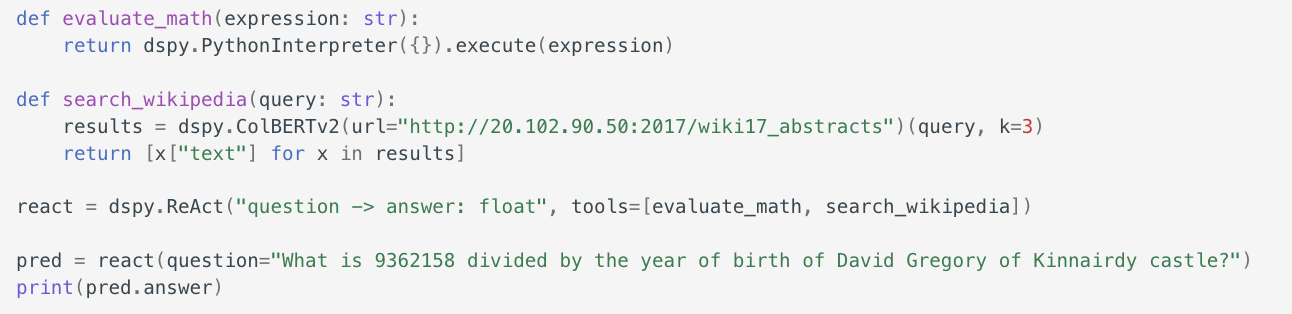
\includegraphics[width=\textwidth]{figures/dspy_react.png}
    \caption{Defining a ReAct agent in DSPy.}
\end{subfigure}

\vspace{0.5em}

\begin{subfigure}[t]{0.95\textwidth}
    \centering
    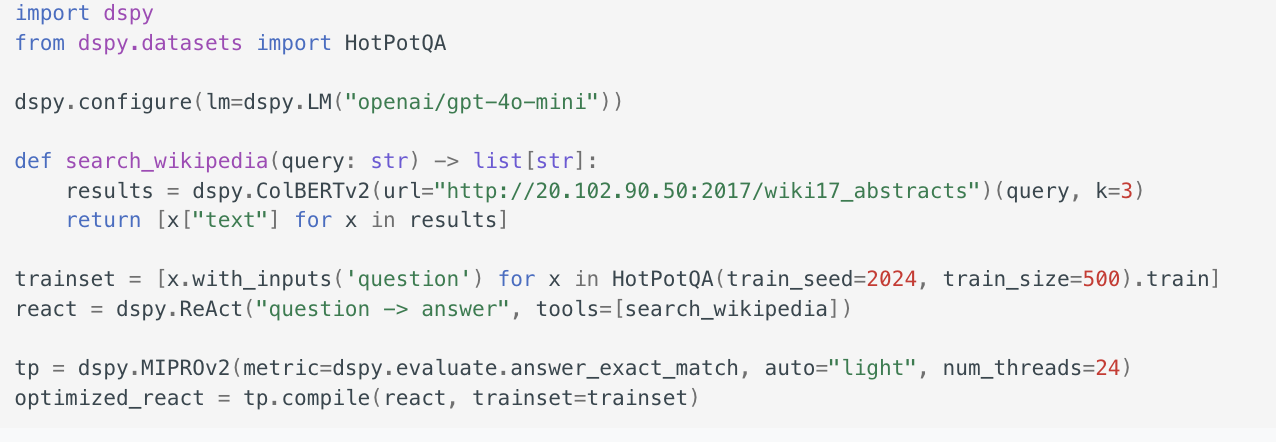
\includegraphics[width=\textwidth]{figures/dspy_optim_react.png}
    \caption{Optimising the ReAct agent using the MIPROv2 optimiser on HotPotQA.}
\end{subfigure}

\caption{Example DSPy workflows for defining and optimising ReAct agents \cite{yao2023reactsynergizingreasoningacting,dspydocs,khattab2023dspycompilingdeclarativelanguage,opsahlong2024optimizinginstructionsdemonstrationsmultistage}.}
\label{fig:dspy-react}
\end{figure}



For instance, a DSPy program for multi-hop question answering was able to improve GPT-3.5’s accuracy by over 25\% compared to a naïve prompt, and even approach GPT-3.5’s level using a 13B open model by optimising its prompts. This underscores the value of optimisation. A smaller model with a good prompt/pipeline can rival a larger model with a bad prompt, whilst also being much cheaper to use.
\newline

While DSPy is powerful, it comes with some engineering trade-offs that have been noted by users. First, adopting DSPy requires writing your entire pipeline using its abstractions (Python classes for Modules, Fields, etc.) rather than your own custom code. This is a heavyweight approach, essentially a new programming paradigm. If a team has already built an agent using another framework (say LangChain or a custom solution), porting it to DSPy could be non-trivial. DSPy’s declarative style introduces a learning curve and some constraints on how you structure the logic. It can also be difficult to debug due to the heavy abstraction and templating layers. Developer experience is a challenge, since a highly abstracted system can disempower developers who then struggle to tweak or understand the hidden prompts. Hiding prompts behind templates doesn’t eliminate prompt engineering; it just moves it out of sight, which can be frustrating if the developer wants fine control. Another limitation is that DSPy, like the algorithms above, still ultimately relies on a scalar metric for optimization. If your application doesn’t have a clear numeric success measure, you’re stuck. In practice, many DSPy examples focus on things like accuracy, F1, or exact match, traditional metrics for QA or classification tasks. If you wanted to optimise, say, a story generation prompt for your idea of “interestingness”, it’s not obvious how to supply a metric for that. So DSPy is great for well-defined tasks with evaluation data, but not directly applicable to open-ended tasks without considerable work and all the challenges in defining a proxy metric.
\newline

The benefit of frameworks like DSPy is that they handle the tedious optimisation logic. The drawback is inflexibility and overhead, you must conform to their structure and trust their abstractions. Some developers might prefer a more lightweight approach where they can plug in an optimisation loop to an existing agent without rewriting it in a new domain specific language. For example, one could envision a tool that wraps around an arbitrary prompt and tries to improve it using human feedback or self-reflection, which could be easier to integrate than a full DSPy rewrite. These observations hint at an opportunity for a more developer-friendly, lightweight optimisation framework that can work with existing agents and leverage richer feedback signals. This leads us to consider approaches that explicitly involve human feedback in the loop.

\section{Human Feedback in Prompt Optimisation}

Involving human feedback is a promising avenue to overcome the limitations of automated metrics in prompt and agent optimisation. After all, humans are the ultimate judges of many tasks (e.g. is a summary accurate and useful? is a chatbot’s answer satisfactory?). Human feedback was instrumental in training aligned language models via Reinforcement Learning from Human Feedback (RLHF) \cite{ouyang2022traininglanguagemodelsfollow} (the technique behind InstructGPT and ChatGPT) where humans provided preference comparisons to shape the model’s behavior. A similar principle can be applied not at the model-parameter level, but at the prompt level: use human preferences or critiques to directly find better prompts that produce outputs humans prefer. This section surveys existing work on prompt optimisation with human feedback, and discusses how it could be expanded both algorithmically and from a user-experience standpoint.
\newline

A recent study explicitly exploring this idea is Prompt Optimization with Human Feedback (POHF) by Lin et al. \cite{lin2024promptoptimizationhumanfeedback}. They consider the setting of a black-box LLM (like an API where you cannot fine-tune the model) that interacts with a user. The goal is to find the optimal prompt to use with that LLM to maximise user satisfaction. The key is they do not assume any automatic reward function; instead, they only rely on human preference comparisons. The algorithm, called APOHF, is inspired by dueling bandits in reinforcement learning. It works like this: it keeps a pool of candidate prompts, and in each iteration, it picks a pair of prompts to test by having the LLM produce responses to some queries using those two prompts. These two responses are then shown to a human (could be the end-user or a human annotator), and the human is asked “Which response do you prefer?” (or which one is better according to some criteria). Based on the human’s choice, the algorithm updates its belief about which prompt is better, and gradually it learns a ranking over the prompt candidates. By clever selection of which prompt pairs to compare next (the dueling bandit strategy ensures we efficiently explore prompts that might be optimal), APOHF homes in on the best prompt after only a small number of comparisons. This is important since human feedback is valuable but expensive, so we want to use it optimally. The results from Lin et al. demonstrated that APOHF could successfully fine-tune prompts for various tasks using very few human preference labels. For instance, they were able to optimise a user instruction prompt to make an LLM’s answers more helpful, and even optimise prompts for text-to-image generation by asking a human which image was more aligned with the request. The big advantage here is no numeric scoring function is needed, humans implicitly provide the “metric” via preferences, which are often far easier to obtain reliably. As the authors note, it’s usually much easier for a person to say “I like output A more than output B” than to assign an absolute score, and preference judgments tend to be more consistent \cite{lin2024promptoptimizationhumanfeedback}. This method still treats the prompt as something to be optimised offline (it’s not adapting on the fly within a single conversation, rather across many test queries), but it shows we can effectively optimise for what users actually care about by involving them.
\newline

\begin{figure}[h]
\centering
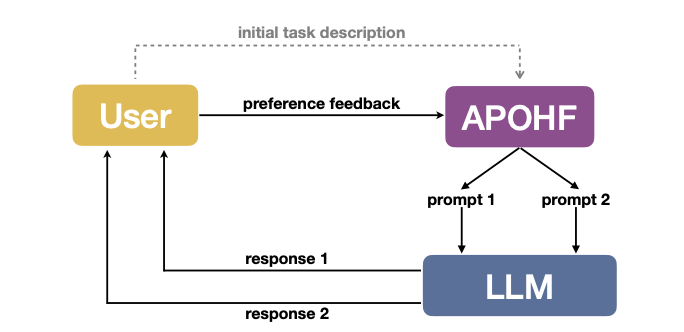
\includegraphics[width=0.6\textwidth]{figures/apohf_overview.png}
\caption{APOHF overview \cite{lin2024promptoptimizationhumanfeedback}}
\end{figure}

Looking forward, we can envision even more interactive and human-centered prompt optimisation approaches. One idea is to allow free-form human feedback on outputs and use an LLM to incorporate that into prompt revisions. Suppose a user says, “The answer you gave is not detailed enough about topic X.” This sentence is extremely informative, more so than a preference or numeric rating. An system could take that feedback and attempt to update the prompt to address it, e.g. by appending an instruction “Always include details about X when relevant.” A simple approach could be to have the LLM read the human’s feedback and generate a suggested prompt edit. This would leverage the model’s ability to interpret human instructions and make the process accessible to non-expert users (who might not know how to write a good prompt from scratch but can certainly say what they didn’t like about the output). 
\newline

Some early research in related directions includes work on learning from explanatory feedback. Where instead of binary preference feedback, the system gets a natural language explanation of what was wrong \cite{scheurer2022traininglanguagemodelslanguage}. This has been studied in the context of model fine-tuning (e.g. using human rationales to guide model updates), but it’s plausible for prompt optimisation too. For example, the GEPA algorithm incorporates self-reflective feedback by having the model generate explanations for its own failures and then revise the prompt accordingly. However, we can hypothesise that human critiques would be substantially more precise. Unlike self-reflection, which may miss fundamental issues or produce vague critiques, human feedback can directly identify the core failure mode and suggest actionable improvements. In domains where quality is subjective and task-specific, this precision could significantly improve both the effectiveness and efficiency of prompt optimisation.
\newline

In terms of user experience, one can imagine a tool integrated into an LLM development process, whenever the agent makes a mistake or produces a subpar response during testing, a developer can annotate it with feedback (like “The agent should have cited the source here” or “This step is redundant”). These annotations would be stored alongside the corresponding inputs, outputs, and execution traces, forming a growing feedback dataset. The optimisation algorithm could then be triggered explicitly by the developer to update prompts or strategies based on the accumulated feedback, or it could even run periodically in the background to incrementally incorporate new annotations without interrupting development. A lightweight framework could allow drop-in usage: e.g., you provide a function / object that generates outputs (your current agent), and the framework helps you systematically improve it by soliciting human feedback.
\newline

We should also note that RLHF for model tuning and prompt optimisation with human feedback are complementary. In RLHF, the model’s weights are adjusted (which is powerful but requires retraining models and can have unintended side-effects on other behaviors). Prompt optimisation is more lightweight. It keeps the model fixed and just updates the prompt. In scenarios where one cannot retrain the model (e.g., using a closed API or lack of training infrastructure), prompt optimisation with human feedback is one of the few avenues to inject alignment/specificity.
\newline

In conclusion, incorporating human feedback into prompt optimisation is an emerging and important direction. Early research like POHF shows that even a simple form (pairwise preferences) can guide prompt search to better satisfy users \cite{lin2024promptoptimizationhumanfeedback}. The opportunities ahead lie in making this process practical and developer friendly, as well as utilising more rich forms of human feedback. This involves developing frameworks where a human (be it an end-user, developer or a domain expert) can easily provide feedback during development or even deployment, and the system can translate that into prompt improvements reliably. If achieved, this would significantly close the loop in the prompt development lifecycle. Developers would be no longer stuck manually fiddling with wording, instead they could leverage both automated search and direct human insight to find on high-performing prompts and agents.
\newline


\chapter{Related Work}
\label{chap:related-work}

\section{Existing Evaluation Libraries and Observability Tooling}
\label{sec:existing_eval_libraries}

Alongside academic benchmarks, several practical libraries have emerged for evaluating LLM applications during development. These tools are useful because they move evaluation closer to the developer workflow: test cases can be rerun, prompts and models can be compared, and failures can be inspected more systematically than with ad hoc scripts. However, they also show that current tooling is still only partially suited to evaluating stateful, tool-using agents.

\subsection{OpenAI Evals}

OpenAI Evals is an open-source framework for evaluating LLMs and LLM systems \cite{openaiEvals}. It provides a general structure for defining datasets, running models on examples, and grading the resulting outputs. This is useful when developers want repeatable evaluation suites for comparing model versions or prompt changes. Evals can also use model-graded checks, where another LLM judges whether the output satisfies some rubric.

The limitation is that OpenAI Evals is still mainly organised around examples and graders. This works well for many single-turn tasks, but is less natural for agent evaluations where the important behaviour may be distributed across several turns, tool calls, and state changes. It can be extended with custom logic, but the framework does not provide a particularly direct scenario-level language for asserting, for example, that a user-facing output, a sequence of tool calls, and the resulting application state are all correct together.

\subsection{DeepEval and Ragas}

DeepEval and Ragas provide more application-oriented evaluation abstractions. DeepEval presents LLM evaluation in a unit-testing style and ships ready-made metrics, including G-Eval \cite{liu2023geval}, alongside measures for RAG, conversations, safety, and agentic behaviour \cite{deepevalDocs}. Its tool correctness metric evaluates whether expected tools were called, with options to consider input parameters and tool outputs \cite{deepevalDocs}.

\begin{figure}[htbp]
  \centering
  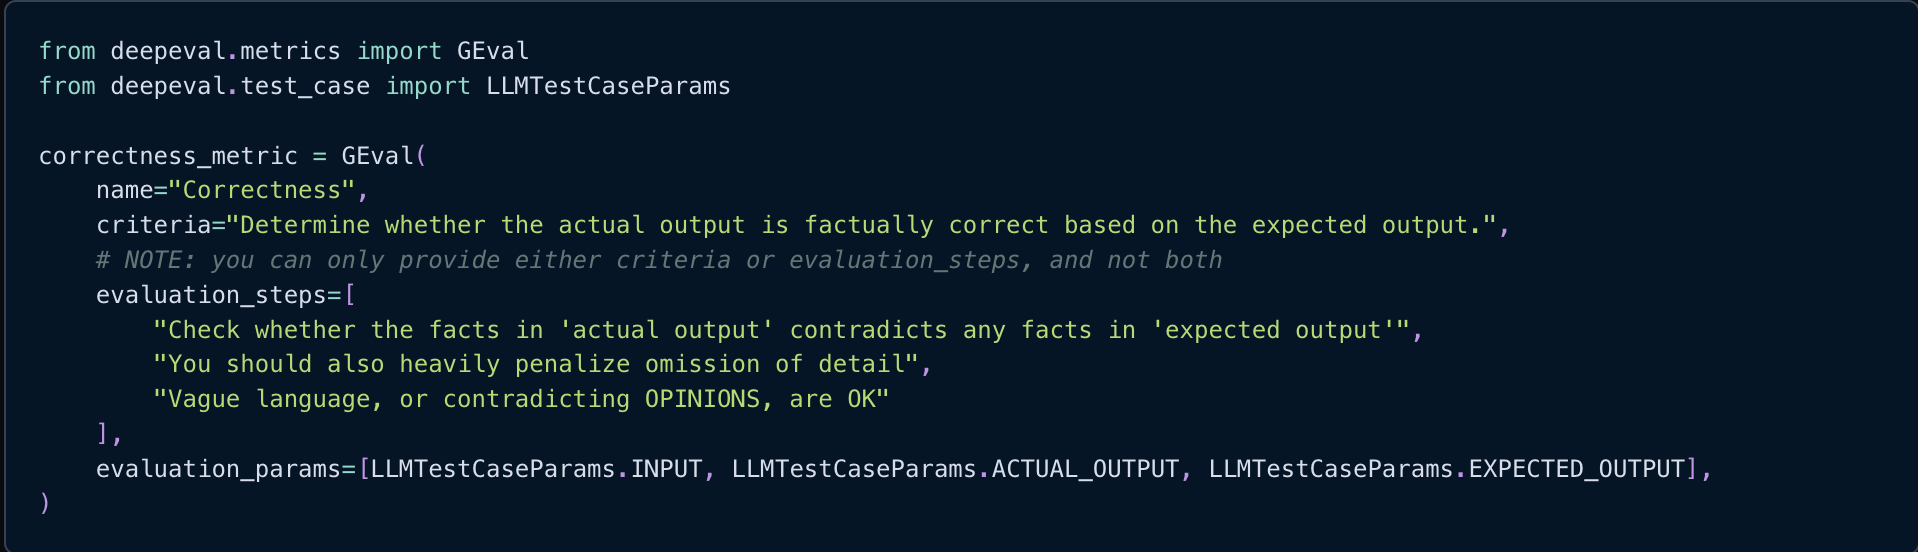
\includegraphics[width=0.8\textwidth]{figures/geval_instantiation_code_snippet.png}
  \caption{G-Eval prompt instantiation using the DeepEval library: evaluation criteria and chain-of-thought instructions are composed into a judge prompt for scoring model outputs \cite{liu2023geval,deepevalDocs}.}
  \label{fig:geval-prompt}
\end{figure}

Ragas was originally designed for RAG evaluation, decomposing quality into dimensions such as faithfulness, answer relevance, context precision, and context recall \cite{es2023ragas,ragasDocs}. More recent versions also include agent metrics such as tool call accuracy, tool call F1, and agent goal accuracy \cite{ragasDocs}. Agent goal accuracy is a binary multi-turn metric: an evaluator LLM reads the full interaction trace, infers the outcome the agent reached, and judges whether it matches the user's goal, either against a provided reference outcome or by inferring the goal from the conversation \cite{ragasDocs}.

These libraries are valuable because they recognise that LLM systems should not only be judged by final-answer quality. However, their tool checks are still relatively metric-oriented. They are useful for comparing expected and actual tool calls, but they are less ergonomic when a developer wants to specify precise properties of a tool argument or a structured output. For example, checking that a particular tool argument contains the substring \texttt{urgent}, or that a nested structured output field satisfies a domain-specific predicate, is not usually a first-class assertion. It generally requires custom code, a custom metric, or reshaping the output into the format expected by the evaluator. This makes simple behavioural expectations feel heavier than ordinary software tests.

\subsection{Promptfoo}

Promptfoo is an open-source tool for evaluating and red-teaming LLM applications using declarative test cases \cite{promptfooDocs}. It supports prompt and model comparison, assertions, CI/CD workflows, caching, and multiple providers. It also includes deterministic assertions such as equality, substring containment, regex matching, JSON validation, and custom JavaScript or Python assertions \cite{promptfooDocs}. This makes it closer to traditional test-driven development than many purely metric-based evaluation frameworks.

Promptfoo is therefore one of the more practical tools for developer-led LLM testing. However, its main abstraction is still the prompt/application test case and its assertions. More complex agent checks, especially those involving multi-turn traces, tool-call arguments, structured outputs, and stateful side effects, can become awkward unless the developer writes custom assertion logic. It provides a useful assertion vocabulary, but it is less focused on representing a full agent scenario as a single object with output checks, tool checks, and state checks expressed together.

\subsection{Observability-Focused Tools}

A related group of tools focuses on observability rather than evaluation alone. LangSmith provides tracing, evaluation, prompt testing, feedback collection, and production monitoring for LLM applications \cite{langsmithDocs}. Langfuse similarly provides open-source application tracing, prompt management, evaluation, user feedback, and monitoring for LLM systems \cite{langfuseDocs}.

\begin{figure}[htbp]
  \centering
  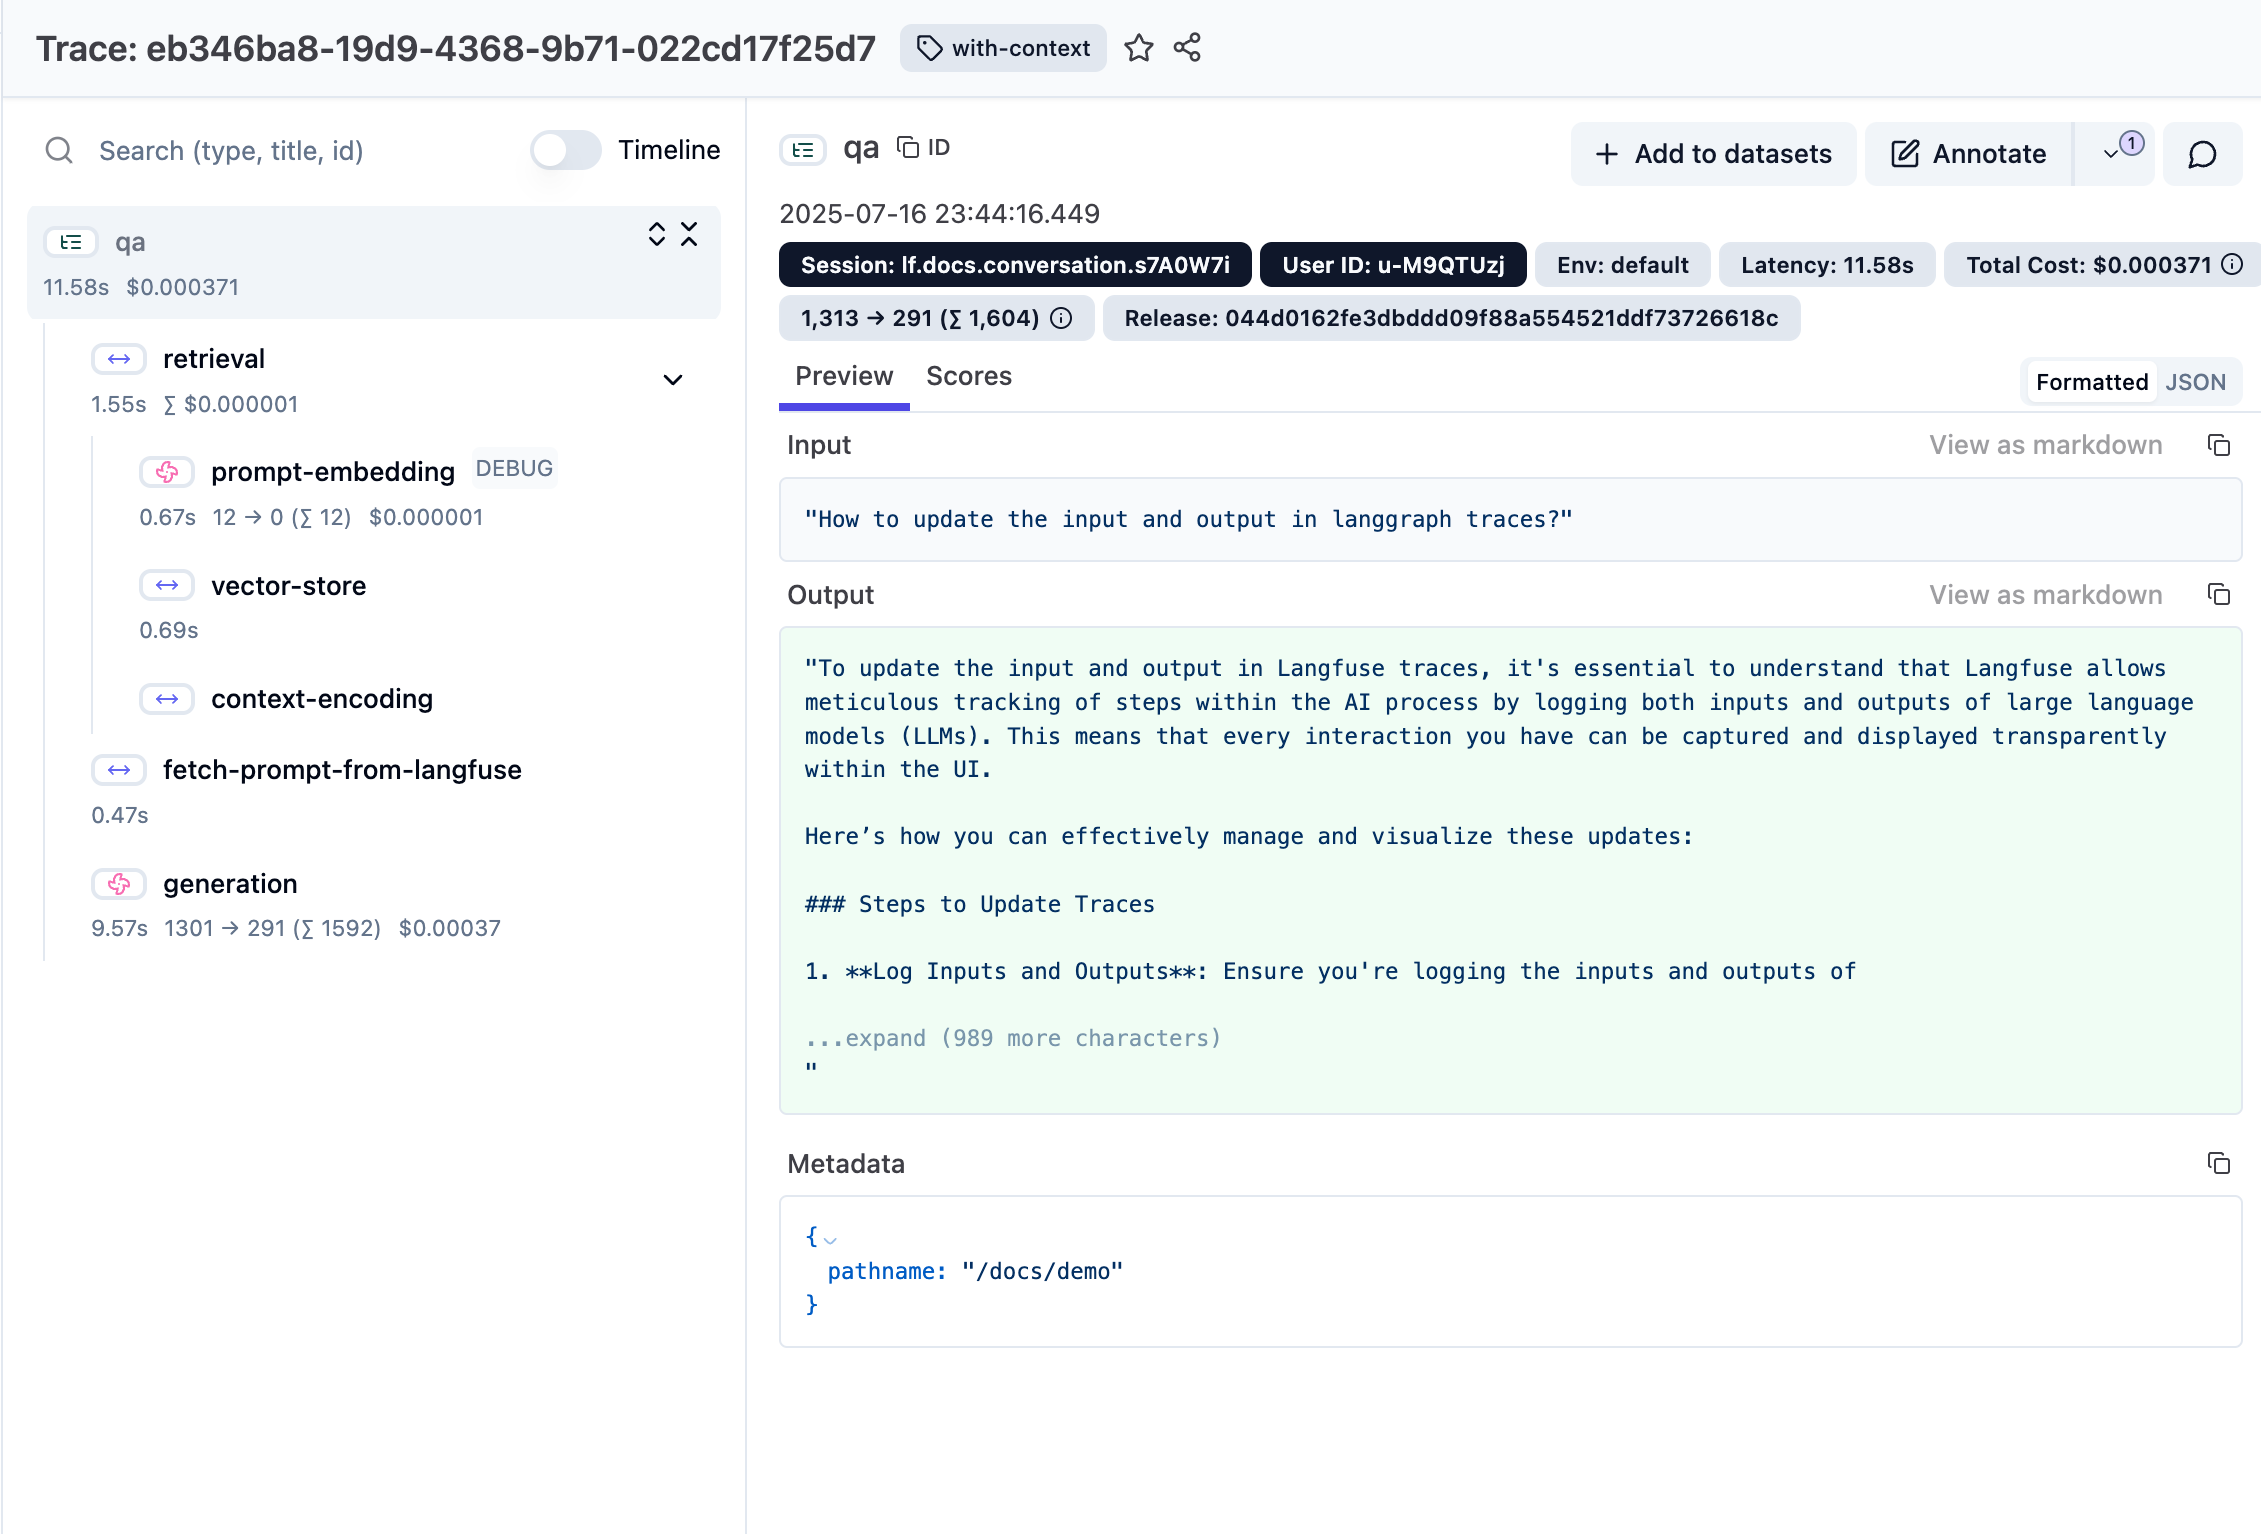
\includegraphics[width=0.88\textwidth]{figures/langfuse_example_trace.png}
  \caption{Example Langfuse trace for a RAG-style QA request: nested observations record retrieval (embedding and vector-store lookup), prompt retrieval, and final generation, with per-step latency, token usage, inputs, outputs, and cost \cite{langfuseDocs}.}
  \label{fig:langfuse-trace}
\end{figure}

These tools are important because agent failures are often hard to understand without seeing the full execution trace: the prompts, model responses, tool calls, tool outputs, intermediate steps, latency, and cost.

Observability tools are therefore highly complementary to evaluation libraries. They help developers inspect what happened during a run. However, observability does not by itself define what should have happened. A trace viewer can show that a tool was called, but the developer still needs a concise way to specify that the tool should only have been called after another condition, that its arguments should satisfy particular properties, that the final output should mention a required concept, and that the external state should end in a valid configuration.

\subsection{Gaps in Existing Libraries}

Existing libraries cover many important parts of the evaluation workflow, but they leave a gap for scenario-driven agent testing. Some tools are strong at scoring final outputs. Others provide RAG or tool-use metrics. Others provide trace observability and production monitoring. What is still missing is a developer-friendly way to define a complete agent scenario and attach explicit checks over the different surfaces of behaviour.

In particular, current tooling does not make it easy enough to combine output assertions, tool-call assertions, and state assertions in one coherent test. A developer should be able to express checks such as: the final response contains a required phrase, a particular tool was called with an argument satisfying a property, a forbidden tool was not called, and the resulting state matches the intended outcome. These checks should be easy to read, easy to modify, and should produce useful diagnostic output explaining which part of the scenario failed.

This is especially important for LLM agents because failures are often not visible in the final response alone. An agent may answer politely while calling the wrong tool, using the wrong argument, skipping a required step, or leaving the system in an invalid state. Conversely, a generic score may indicate failure without showing whether the problem was in the output, the tool trajectory, or the state transition. The main gap is therefore not simply the absence of metrics, but the absence of concise scenario-style evaluation tooling that treats the full agent trace as the object being tested.

\section{Motivation for Agent-Spec-Kit}
\label{sec:agent-spec-kit-motivation}

Chapter~\ref{chap:background} argues that agent evaluation must cover traces, tools, state, and repeated runs, not only final answers. Benchmarks such as AppWorld, $\tau$-bench, and ToolSandbox show why \cite{trivedi2024appworld,yao2024taubench,lu2024toolsandbox}; software-testing work shows how to find, simplify, and preserve failures \cite{claessen2000quickcheck,zeller2002simplifying,yu2023gptfuzzer,yao2023fuzzllm}. The preceding section shows that existing libraries and observability tools still do not make it easy to express those checks together in one scenario.

The remaining gap is developer-facing: a way to specify, run, inspect, and rerun behavioural tests for a custom agent without adopting a fixed benchmark or writing large amounts of custom glue code. Agent-Spec-Kit targets that gap. It treats an agent episode as a testable scenario with explicit checks over the final output, tool calls, and environment state, and it supports workflows such as repeated trials, generative variation, failure shrinking, and regression extraction described in the methodology chapter.

\chapter{Methodology}
\label{chap:methodology}

\section{Design Goals and Requirements}
\label{sec:design-goals}

Chapter~\ref{chap:related-work} argues that developers evaluating tool-using agents need more than aggregate scores or trace viewers. They need a single scenario in which output checks, tool checks, and state checks can be written together, and when something fails they need to know which expectation broke. Chapter~\ref{chap:background} shows why that need arises: agent correctness is spread across final messages, tool trajectories, and environment state, and failures on one turn may be hidden by recovery on a later turn. This section states the design goals that follow from that gap and contrasts how existing tools report failures with the response built into \emph{agent-spec-kit}.

\subsection{Functional Requirements}

The framework is intended to support evaluation workflows that resemble software testing more than benchmark leaderboards. Concretely, a developer should be able to express expectations over the user-facing output, the sequence of tool calls (including nested specialist subgraphs), and postconditions on databases or other fixtures, using one composable matcher language rather than ad hoc glue per check. When an assertion fails, the report should identify the failing step and turn, qualify the mismatch with a path into structured data (for example \texttt{\$.args.line\_id}), and attach enough transcript and event context to decide whether to change a prompt, a graph edge, or a policy document.

The same scenario file should read as a conversation script: explicit user lines, checks after each agent turn, optional environment mutations between turns, and optional generative extensions when user behaviour should vary. Repeated runs of the same script support stochastic agents; generative fuzzing and user simulation extend the script without changing the assertion vocabulary. Integrations for LangChain and Pydantic AI normalize traces so those assertions do not depend on framework-specific message formats.

These goals deliberately exclude building a new fixed benchmark suite (evaluation of TelcoSupportBench appears in the Evaluation chapter), prompt optimisation, or replacement of observability products such as Langfuse. The framework complements trace inspection by stating what should have happened at the point of failure.

\subsection{Diagnostics Compared with Existing Libraries}

Table~\ref{tab:diagnostics-comparison} summarises how several common evaluation patterns report failure and what is still awkward when debugging a custom agent. The point is not to claim that other tools are inadequate in general, but to motivate why \emph{agent-spec-kit} invests in assertion-local counterexamples.

\begin{table}[htbp]
\centering
\small
\renewcommand{\arraystretch}{1.2}
\begin{tabularx}{\textwidth}{p{0.22\textwidth}p{0.36\textwidth}X}
\toprule
\textbf{Tool / pattern} & \textbf{What you get on failure} & \textbf{Limitation for agent debugging} \\
\midrule
DeepEval / Ragas metrics &
Scalar score and metric name &
Hides which tool or argument failed; component metrics rarely give a path at the assertion site. \\
G-Eval / LLM-as-judge &
Numeric or rubric score &
Strong for open-ended text; weak for precise tool-argument or state facts (Chapter~\ref{chap:background}, \S\ref{sec:bg-oracles}). \\
Promptfoo &
Pass/fail per assertion; trajectory checks via OTLP traces &
Powerful, but trace assertions sit apart from the scenario script; multi-assertion scenarios require span navigation. \\
LangSmith / Langfuse &
Rich trace trees, latency, cost &
Shows what happened; the developer still infers expected behaviour (Figure~\ref{fig:langfuse-trace}). \\
Fixed benchmarks ($\tau$-bench, AppWorld) &
Task pass/fail, sometimes action logs &
Less reusable for bespoke agents; dual-control setups such as $\tau^2$-bench~\cite{barres2025tau2} embed orchestration in the benchmark rather than a general test DSL. \\
\bottomrule
\end{tabularx}
\caption{How common evaluation patterns report failure, and why assertion-local diagnostics remain useful for custom agents.}
\label{tab:diagnostics-comparison}
\end{table}

\emph{agent-spec-kit} responds by attaching a structured \emph{Counterexample} to each failed scenario assertion: a headline, a human-readable location (for example which \texttt{assert\_tool\_calls} ran after turn three), an optional JSON-pointer path, expected and actual summaries, notes (including per-criterion judge rationales), and a bounded event trace. Matchers are composable so inner failures surface with deeper paths. Section~\ref{sec:counterexamples} describes that pipeline; the intended workflow is to read the path, inspect the trace, change the agent or policy, rerun under a named experiment, and compare outcomes in the web UI (Section~\ref{sec:execution-workflow}).

\section{System Architecture}
\label{sec:architecture}

Before describing how the library is wired together, it helps to see what a developer actually writes. Listing~\ref{lst:architecture-motivating} shows a compact scenario. A fixture supplies the agent under test, the scenario declares how many times to run it, and the body chains user lines with expectations on tools and reply text.

\begin{lstlisting}[language=Python,caption={Scenario with fixture, repeats, user line, tool and output checks.},label=lst:architecture-motivating]
@ek.fixture
async def adapted_agent():
    return wrap_langchain_agent(
        tutor_graph,
        lambda msg: {"messages": [HumanMessage(content=msg)]},
    )

@ek.scenario(
    agent_fixture="adapted_agent",
    repeats=3,
    tags=("smoke",),
    timeout_s=90.0,
)
async def test_multiply_dialog_scripted_user_messages(s):
    (
        s.user_message("What is 5 x 6?")
        .assert_tool_calls(
            [m.tool_call("multiply_integers", args={"a": 5, "b": 6})],
            ordered=True,
            allow_extras=True,
        )
        .assert_output(m.contains("30"))
    )
\end{lstlisting}

Expectations in the scenario body use matchers from the library's match module, imported as \texttt{import agent\_spec\_kit.match as m} and written \texttt{m} in listings for brevity (Section~\ref{sec:match-system}). The fixture injects a LangGraph tutor wrapped as an \texttt{AdaptedAgent} so the scenario body can focus on behaviour rather than wiring. \texttt{repeats=3} schedules three independent executions of the same script, which is useful when the underlying LLM is stochastic and a single lucky pass is not enough evidence. The scenario body is the behavioural contract. After the user asks for $5 \times 6$, the tutor must call \texttt{multiply\_integers} with the right arguments and mention the product in its reply. Failures on either the tool trace or the final text produce a counterexample at that assertion (Section~\ref{sec:counterexamples}). The rest of this section explains how those declarations are discovered, executed, and checked. Optional generative extensions (simulated users, fuzzing, shrinking) are described later in Section~\ref{sec:generative}.

\subsection{End-to-End Pipeline}

\emph{agent-spec-kit} is organised as a pipeline from decorated Python test modules through scenario execution to persisted results. The architecture keeps three concerns separate, namely discovering and running scenarios, normalising agent behaviour into typed events, and checking behaviour with composable matchers that produce structured failures when expectations are not met. Figure~\ref{fig:methodology-architecture} sketches that core path.

\begin{figure}[htbp]
  \centering
  \resizebox{0.72\textwidth}{!}{%
    % Shared TikZ styles for methodology flow diagrams
\tikzset{
  flow/.style={
    rectangle,
    draw=black!70,
    rounded corners=2pt,
    fill=blue!4,
    minimum height=8mm,
    inner sep=4pt,
    align=center,
    font=\small,
    text width=2.6cm,
  },
  flowwide/.style={
    flow,
    text width=3.4cm,
  },
  flownarrow/.style={
    flow,
    text width=2.1cm,
  },
  store/.style={
    flow,
    fill=green!6,
    text width=2.8cm,
  },
  fail/.style={
    flow,
    fill=red!8,
    text width=2.5cm,
  },
  arr/.style={-{Stealth[length=2.2mm]}, thick, draw=black!65},
  lbl/.style={font=\footnotesize, fill=white, inner sep=1pt},
}
%
    \begin{tikzpicture}[
  node distance=5mm,
  arr/.style={-{Stealth[length=2.2mm]}, thick, draw=black!65},
]
  \node[flow] (dec) {\texttt{@fixture} /\\\texttt{@scenario}};
  \node[flow, below=of dec] (cli) {CLI \texttt{run}};
  \node[flow, below=of cli] (job) {\texttt{run\_scenario\_job}};
  \node[flow, below=of job] (mat) {\texttt{Scenario.}\\\texttt{materialise}};
  \node[flow, below=of mat] (agent) {\texttt{AdaptedAgent}\\\texttt{run\_turn}};
  \node[flow, below=of agent] (match) {\texttt{match.}\\\texttt{async\_check}};

  \node[fail, below left=10mm and 4mm of match] (rec) {\texttt{FailureRecord}};
  \node[fail, below=of rec] (cx) {\texttt{Counterexample}};
  \node[fail, below=of cx] (out) {CLI panel /\\SQLite / UI};

  \node[store, below right=10mm and 4mm of match] (store) {\texttt{LocalResultStore}};

  \draw[arr] (dec) -- (cli);
  \draw[arr] (cli) -- (job);
  \draw[arr] (job) -- (mat);
  \draw[arr] (mat) -- (agent);
  \draw[arr] (agent) -- (match);
  \draw[arr] (match) -- node[lbl, above, sloped] {fail} (rec);
  \draw[arr] (rec) -- (cx);
  \draw[arr] (cx) -- (out);
  \draw[arr] (match) -- node[lbl, above, sloped] {ok} (store);
\end{tikzpicture}
%
  }
  \caption{Core execution flow from \texttt{@scenario} registration through matching and result storage. Failed assertions branch to structured counterexamples shown in the CLI and web UI.}
  \label{fig:methodology-architecture}
\end{figure}

Developers register fixtures and scenarios with decorators (\texttt{@fixture}, \texttt{@scenario}). The CLI command \texttt{agent-spec-kit run} discovers \texttt{test\_*.py} files, resolves fixture dependencies, and schedules one job per scenario case and repeat index. Each job builds a \texttt{Scenario} instance, runs the scenario function (which queues steps such as \texttt{user\_message} and \texttt{assert\_tool\_calls}), and calls \texttt{materialise()} to execute those steps in order.

For each \texttt{user\_message}, the runner invokes \texttt{AdaptedAgent.run\_turn}, which returns a \texttt{TurnResult} with user-visible output and a tree of \texttt{AgentTurnEvent} and \texttt{ToolCallEvent} nodes. Assertion steps call \texttt{match.async\_check} on outputs, tool-call lists, or environment functions. On success the runner advances to the next queued step and eventually records a pass in the local result store. On failure the pipeline branches before that pass is written.

\subsection{Failure Path and Main Modules}

The failure path is deliberately three-layered so matchers stay reusable and reporting stays stable. Matchers emit \texttt{MatchError} values with JSON-pointer paths and optional witness JSON. The scenario runner wraps those in a \texttt{FailureRecord} that records which step kind failed, which turn and assertion index applied, and a snapshot of the transcript. \texttt{counterexample\_from\_failure} then produces the developer-facing \texttt{Counterexample} consumed identically by the CLI Rich panel and the web FailureCard. Section~\ref{sec:counterexamples} develops that story in full.

The implementation is split across modules so each layer can evolve independently. \texttt{scenario\_core.py} implements the fluent scenario DSL and step dispatch. \texttt{runner.py} orchestrates jobs, fixture teardown, and timeouts. \texttt{match/} implements coercion, object and list matchers, tool-call shapes, LLM criteria judges, and readable rendering of matcher specs for failure panels. \texttt{failures.py} and \texttt{cli\_reporting.py} turn matcher errors into developer-facing panels. \texttt{integrations/} adapts LangChain and Pydantic AI graphs to the event model. \texttt{cli.py} and \texttt{result\_store.py} persist run metadata, transcripts, and counterexample blobs under \texttt{.agent\_spec\_kit/}.

The next sections unpack the scenario language and matchers introduced in Listing~\ref{lst:architecture-motivating}, then counterexamples, integrations, optional generative features, and the execution workflow.

\section{The Scenario Language for Scripting Conversations}
\label{sec:scenario-language}

The central interface of \emph{agent-spec-kit} is a scenario language implemented as fluent Python on a \texttt{Scenario} object. A scenario file should read top to bottom like a transcript with expectations woven in. Seed the environment state, send a user line, check tools and reply, optionally change the environment, send another line, and check again. That ordering matches how engineers describe multi-turn bugs in practice and avoids splitting conversation logic in YAML while assertions live elsewhere, which Chapter~\ref{chap:related-work} identifies as a common friction point in some libraries.

\subsection{Scripting Metaphor and Developer Ergonomics}

Scenarios are plain \texttt{async def test\_*} functions decorated with \texttt{@scenario}, with dependencies injected through \texttt{@fixture} in the same style as pytest. Steps such as \texttt{user\_message} and \texttt{assert\_tool\_calls} are chained on \texttt{s} and executed when \texttt{materialise()} runs (the runner usually does this implicitly after the scenario body returns). Queuing before execution lets the generative layer record a scenario once and replay it with different generated user lines without rewriting the assertion block.

Because the language is Python, conversation and oracles stay in one module that refactors with the rest of the test suite. The agent under test does not need to import the framework. Only the test file declares the behavioural contract. That lowers adoption cost compared with frameworks that require wrapping production agents in heavyweight abstractions.

\subsection{Multi-Turn Scripted Conversations}

Listing~\ref{lst:multiply-dialog-scripted} shows a minimal two-turn script. After each user message the scenario requires a specific tool call and a reply that contains the expected product.

\begin{lstlisting}[language=Python,caption={Two-turn scripted scenario with per-turn tool and output checks.},label=lst:multiply-dialog-scripted]
(
    s.user_message("What is 5 x 6?")
    .assert_tool_calls(
        [m.tool_call("multiply_integers", args={"a": 5, "b": 6})],
        ordered=True,
        allow_extras=True,
    )
    .assert_output(m.contains("30"))
    .user_message("What is 9 x 8?")
    .assert_tool_calls(
        [m.tool_call("multiply_integers", args={"a": 9, "b": 8})],
        ordered=True,
        allow_extras=True,
    )
    .assert_output(m.contains("72"))
)
\end{lstlisting}

Each \texttt{user\_message} triggers one agent turn and appends to the transcript. By default, \texttt{assert\_output} and \texttt{assert\_tool\_calls} apply to the most recent agent turn (\texttt{turn="last"}). For dialogue-wide checks, set \texttt{turn="up\_to\_now"}. \texttt{actor=} selects agent or user lines. Mixing tool and output assertions after the same user line is deliberate because many agent failures are visible only in the trace even when the final sentence sounds acceptable (Chapter~\ref{chap:background}).

\subsection{Environment Setup and Mid-Scenario Actions}

Scenarios also describe world state, not only dialogue. Table~\ref{tab:env-step-types} contrasts three mechanisms.

\begin{table}[htbp]
\centering
\small
\begin{tabularx}{\textwidth}{p{0.18\textwidth}p{0.22\textwidth}p{0.14\textwidth}X}
\toprule
\textbf{Mechanism} & \textbf{When} & \textbf{Pass/fail?} & \textbf{Role} \\
\midrule
\texttt{@fixture} & Before scenario body & -- &
Inject isolated stores, agents, flags, then \texttt{yield} teardown. \\
\texttt{s.action(fn)} & Any queued step & No &
Side effect on environment. Receives fixture kwargs. \\
\texttt{s.assert\_that(fn)} & Any queued step & Yes &
Same call pattern as \texttt{action}. Failure yields a counterexample. \\
\bottomrule
\end{tabularx}
\caption{Fixtures, actions, and environment assertions in the scenario script.}
\label{tab:env-step-types}
\end{table}

Listing~\ref{lst:action-assert} illustrates \texttt{action} followed by \texttt{assert\_that}. The test simulates an external change (a ticket inserted into a store) and then checks that the store satisfies a postcondition.

\begin{lstlisting}[language=Python,caption={Mid-scenario environment mutation and state check.},label=lst:action-assert]
def _apply_state() -> None:
    insert_ticket(ticket_store, line_id=meta()["line_id"])

(
    s.user_message("check")
    .action(_apply_state)
    .assert_that(lambda: assert_ticket_exists(ticket_store))
)
\end{lstlisting}

That pattern supports offline user effects (a device reboot, a payment posted outside the chat) without building a full user simulator, and it supports ordering constraints such as verifying that the agent did not mutate state before authentication.

Dual-control evaluation, where both agent and user can change shared state through tools, appears in $\tau^2$-bench~\cite{barres2025tau2}. The scenario language can express the same pattern with a \texttt{user\_fixture} with its own tools and \texttt{simulate\_conversation}, scripted \texttt{action} steps for deterministic user-side effects, and \texttt{assert\_that} on a shared store after both parties have acted. Chapter~\ref{chap:background} contrasts $\tau$-bench-style single-control users with this richer interaction model. The empirical study in this project uses a single-control telecom setup, but dual-control scenarios can be written with these fixtures and steps today.

\subsection{Registration, Discovery, and Repeats}

\texttt{@scenario} binds \texttt{agent\_fixture} and optionally \texttt{user\_fixture}, and sets \texttt{repeats}, \texttt{tags}, and timeouts. Discovery imports \texttt{test\_*.py} and \texttt{fixtures.py} recursively, registering definitions in global registries before execution.

\texttt{repeats=N} schedules \texttt{N} independent jobs for the same case, useful when the same scenario may pass or fail on different runs because the model is not deterministic. Run summaries report how many of those jobs passed.

\subsection{Parametrized Fixtures}

When the same conversation script should run against several LLM backends, seeds, or configuration tuples, duplicating the scenario body is wasteful and hard to maintain. \texttt{@parametrize} on a fixture (or on \texttt{@scenario}) expands one registered definition into multiple cases, each with its own job row in run summaries and the Compare UI.

Listing~\ref{lst:parametrize-fixture} shows the idea. The scenario in Listing~\ref{lst:architecture-motivating} stays unchanged while only the fixture varies the model passed into the wrapped graph.

\begin{lstlisting}[language=Python,caption={Parametrized agent fixture: one scenario, multiple model cases.},label=lst:parametrize-fixture]
_LLM_MODEL_CASES = (
    ek.case("gpt-4.1-nano-2025-04-14", id="gpt41nano"),
    ek.case("gpt-5-nano", id="gpt5nano"),
)

@ek.fixture
@ek.parametrize("llm_model", _LLM_MODEL_CASES)
async def adapted_agent(llm_model: str):
    return wrap_langchain_agent(build_tutor_graph(llm_model), ...)
\end{lstlisting}

Parametrization is orthogonal to \texttt{repeats}. A parametrized case can still set \texttt{repeats=3} to estimate pass rate for that model, whereas repeats without parametrization re-runs the identical configuration. Section~\ref{sec:execution-workflow} describes how runs and experiments surface those rows when comparing agent updates across models or prompts.

\section{Match System for Composable Oracles}
\label{sec:match-system}

Scenarios declare \emph{what} should hold. The match system decides whether observed behaviour satisfies those declarations and, when it does not, produces structured errors that feed counterexamples (Section~\ref{sec:counterexamples}). The design goal is expressiveness through composability. One small vocabulary of matchers should cover substring checks, JSON-shaped outputs, ordered or unordered tool lists, nested tools from specialist agents, forbidden tools, and selective LLM rubrics, without bespoke Python per check. That aligns with the oracle types summarised in Table~\ref{tab:agent-oracle-types} in Chapter~\ref{chap:background}.

\subsection{Specs and Combinators}

Each \texttt{assert\_output} or \texttt{assert\_tool\_calls} step takes a \emph{spec}, meaning a description of what the agent should have produced. Authors can write that description in two ways. Plain Python values are interpreted as matchers on their own. A string means the value must equal that string, a dict becomes an \texttt{m.object} field check, and a list becomes an ordered \texttt{m.list}. For richer checks, logical combinators such as \texttt{m.all\_of}, \texttt{m.one\_of}, and \texttt{m.not\_} combine primitive matchers such as \texttt{m.contains} and \texttt{m.regex}. Listing~\ref{lst:match-combinators} shows a refund reply where several output constraints apply at once.

\begin{lstlisting}[language=Python,caption={Combining substring, negation, and regex constraints on one output.},label=lst:match-combinators]
m.all_of(
    m.contains("refund"),
    m.not_(m.contains("guaranteed")),
    m.regex(r"within \d+ business days"),
)
\end{lstlisting}

Combinators express logical structure. \texttt{all\_of} requires every child matcher to pass, \texttt{one\_of} accepts any one of them, and \texttt{not\_} negates a constraint. When a built-in matcher is not enough, \texttt{m.match(fn, message=...)} wraps a small predicate with a custom failure message. Primitives such as \texttt{contains}, \texttt{regex}, \texttt{string} with length bounds, and \texttt{number} with ranges cover common checks on both final replies and partially specified tool arguments.

\subsection{Object Matching and Structured Output}

\texttt{m.object} checks field shapes on dict-like or Pydantic views. The \texttt{extra=} policy controls whether unknown keys are ignored or rejected, and \texttt{m.optional} marks a field that may be absent. Conditional rules from \texttt{m.require} and \texttt{m.forbid} with \texttt{m.field(...).when(...)} express implications such as requiring the \texttt{"pager\_group"} field when \texttt{"severity"} is \texttt{"high"}.

Listing~\ref{lst:match-object} shows structured ticket metadata with an unordered component list and a conditional rule.

\begin{lstlisting}[language=Python,caption={Object matcher with conditional rules.},label=lst:match-object]
m.object(
    {
        "ticket": m.object(
            {
                "severity": m.one_of("high", "medium"),
                "components": m.list(
                    ["edge", "core"], mode="unordered", allow_extras=False
                ),
            },
            rules=[
                m.require("pager_group").when(m.field("severity") == "high"),
            ],
        )
    },
    extra="forbid",
)
\end{lstlisting}

Nested \texttt{m.object} specs mirror nested agent outputs. Each layer contributes path segments on failure (for example \texttt{\$.itinerary[1].day} within the parsed output value the matcher checked), so the counterexample can point inside a large JSON body rather than reporting only that the object did not match. When an outer object fails because an inner field fails, error selection prefers the deepest path so the headline can combine an outer error summary, the nested path, and an inner error summary (for example \texttt{outer summary; mismatch at \$.foo: inner summary}).

When agents return structured payloads from tools or coordinators, these matchers implement the structured-output checks in Table~\ref{tab:agent-oracle-types}.

\subsection{List and Tool-Call Matching}

\texttt{m.list} checks whether an actual sequence matches an expected one. In order mode, the spec sequence must appear as a subsequence when \texttt{allow\_extras=True}, or as an exact length match when extras are disallowed. In unordered mode, every listed item must appear the required number of times, but may appear in any order. That suits parallel tools that may complete in either sequence. \texttt{m.list\_of} is the homogeneous case in which one inner spec is applied to every item in the run. Listing~\ref{lst:match-list-of} shows a structured output check where every alert in an \texttt{alerts} array must carry one of three allowed severity levels.

\begin{lstlisting}[language=Python,caption={\texttt{m.list\_of}: every item in the list must satisfy the same inner spec (here, each alert object must have \texttt{severity} set to \texttt{low}, \texttt{medium}, or \texttt{high}).},label=lst:match-list-of]
m.list_of(
    m.object({"severity": m.one_of("low", "medium", "high")})
)
\end{lstlisting}

Tool assertions build on those list matchers. Each recorded call is matched as a small dictionary with \texttt{name}, \texttt{args}, \texttt{result}, and \texttt{children} for calls made on behalf of a parent tool (for example by a specialist agent). \texttt{m.tool\_call} describes one such entry. For \texttt{args} (and \texttt{metadata}), a plain \texttt{dict} is treated as \texttt{m.object(..., extra="ignore")}, so only the listed keys are checked and additional keys on the actual call are allowed. Pass \texttt{m.object} explicitly when you need \texttt{extra="forbid"} or conditional rules. An \texttt{assert\_tool\_calls} spec is a list of those descriptions (using \texttt{m.list} under the hood). Nested \texttt{children} follow the same pattern. A parent \texttt{m.tool\_call} can require a nested list of child calls, each with its own argument and result checks. Listing~\ref{lst:match-tool-nested} shows that layout.

\begin{lstlisting}[language=Python,caption={Nested tool-call spec with child tools.},label=lst:match-tool-nested]
m.tool_call(
    "run_forensics_specialist",
    args={"query": m.contains("latency")},
    children=[
        m.tool_call("pull_logs", args={...}),
        m.tool_call(
            "score_anomaly",
            result=m.llm_criteria(
                criteria=[
                    "mentions a numeric anomaly score or risk band",
                    "does not state root cause as certain fact",
                ],
                threshold=2,
                model="openai:gpt-5-nano",
            ),
        ),
    ],
)
\end{lstlisting}

\texttt{forbid\_tool\_calls} expresses negative expectations (a credit tool must not appear). When the list length differs from the spec, witness metadata on the matcher error can name expected versus actual tool sequences, which feeds readable summaries in the failure panel as described in Section~\ref{sec:matcher-spec-repr}. That shared dictionary shape is what lets the same \texttt{m.tool\_call} spec run against any integrated agent stack without scenario changes.

Function-calling benchmarks such as BFCL~\citep{patil2025bfcl} check argument trees against schemas. The match layer generalises that idea to partial specs and incomplete traces where only some fields matter for policy.

\subsection{LLM Criteria Judges and G-Eval-Style Scoring}

Some properties are hard to express with fixed matchers, such as tone, hedging, or whether a free-form specialist summary addresses the user's concern without overclaiming. For those cases \texttt{m.llm\_criteria} asks a judge model yes/no questions on several narrow criteria and passes if at least \texttt{threshold} succeed (by default, all must). This differs from G-Eval-style pipelines (Figure~\ref{fig:geval-pipeline} and Figure~\ref{fig:geval-prompt}), which often map rubric text to numeric ratings via token probabilities. When a criterion fails, the judge returns a short rationale that appears in the counterexample notes. That is easier to act on than a single opaque score and tends to be more stable than open-ended ratings for small, well-scoped questions.

\texttt{m.llm\_criteria} fits where nuance is required and a deterministic rule over free-form text would be brittle or unreadable, not where the expectation is already a machine fact such as a tool name, a structured field, or a database postcondition. Authors may attach it to a specialist tool result or the agent's final reply while keeping deterministic checks on trace and state in the same scenario. Chapter~\ref{chap:background} cautions that LLM judges should not replace machine-level oracles. They should be reserved for subjective rubrics, not for facts that \texttt{m.object}, \texttt{m.tool\_call}, or \texttt{assert\_that} can state directly.

\subsection{Mapping Assertions to Oracle Surfaces}

Table~\ref{tab:assertion-mapping} links scenario methods to the oracle surfaces introduced in Chapter~\ref{chap:background} (Section~\ref{sec:bg-oracles}, Table~\ref{tab:agent-oracle-types}).

\begin{table}[htbp]
\centering
\small
\begin{tabularx}{\textwidth}{p{0.26\textwidth}p{0.28\textwidth}X}
\toprule
\textbf{Scenario mechanism} & \textbf{Oracle surface} & \textbf{Typical use} \\
\midrule
\texttt{assert\_output} & Final or cumulative text / JSON &
User-facing reply, structured coordinator payloads. \\
\texttt{assert\_tool\_calls} / \texttt{forbid\_tool\_calls} &
Tool trace &
Order, arguments, nested specialist tools. \\
\texttt{assert\_that} & Environment state &
Database rows, flags, collateral-damage checks. \\
\texttt{m.llm\_criteria} & Rubric-based quality &
Subjective tool results, dialogue stop conditions. \\
\bottomrule
\end{tabularx}
\caption{How scenario assertions map to oracle types.}
\label{tab:assertion-mapping}
\end{table}

\subsection{Expressiveness Intent}

Chapter~\ref{chap:evaluation} compares how many lines are required to express the same twelve policy checks (C01--C12) in \emph{agent-spec-kit} and in several other evaluation styles (Section~\ref{sec:expressiveness}). Those checks were chosen because they mix output constraints, structured specialist results, forbidden tools, ordered and unordered tool sequences, and database postconditions. The methodology takeaway is that the matcher vocabulary was designed so those policies compose from \texttt{object}, \texttt{tool\_call}, and list combinators rather than from one-off custom code per check.

\section{Counterexamples and Diagnosability}
\label{sec:counterexamples}

Section~\ref{sec:design-goals} argued that scalar metrics and raw traces leave a gap when debugging custom agents. This section describes how \emph{agent-spec-kit} closes that gap at the assertion that failed: each failed \texttt{assert\_output}, \texttt{assert\_tool\_calls}, \texttt{forbid\_tool\_calls}, or \texttt{assert\_that} yields a \texttt{Counterexample} intended to support an edit-test loop on prompts, graphs, and policies.

\subsection{Design Principles}

A useful failure report should locate the failing step and turn, pinpoint the field path inside structured data, contrast expected and actual values, provide enough transcript and event context to see what the agent did, and phrase the headline so a developer can infer what to change. Observability tools excel at the third item in isolation; they show latency, tokens, and nested spans (Figure~\ref{fig:langfuse-trace}). Assertion-local counterexamples add the first two items at the check that was written in the scenario, so the developer does not manually correlate spans with test intent.

\subsection{Failure Pipeline}

When a matcher fails, \texttt{match.async\_check} returns a \texttt{MatchResult} with one or more \texttt{MatchError} objects carrying paths, codes, and optional witness JSON. The scenario runner wraps that in a \texttt{FailureRecord}: \texttt{step\_kind} distinguishes output, tool, environment, or runtime failures; \texttt{turn\_index} and \texttt{assertion\_index\_after\_turn} locate the failing check in the script; \texttt{matcher\_errors} and \texttt{actual} preserve machine-readable detail; \texttt{turn\_results} holds the transcript window used for display. \texttt{counterexample\_from\_failure} maps that record into the payload shown to developers. Table~\ref{tab:counterexample-fields} lists the main \texttt{Counterexample} fields and why each exists.

\begin{table}[htbp]
\centering
\small
\begin{tabularx}{\textwidth}{p{0.28\textwidth}X}
\toprule
\textbf{Field} & \textbf{Diagnostic role} \\
\midrule
\texttt{headline} &
One-line summary of the first or deepest mismatch. \\
\texttt{location\_detail} &
Human-readable placement (e.g.\ second \texttt{assert\_tool\_calls} after turn 3). \\
\texttt{path} &
JSON-pointer into structured actuals (\texttt{\$.args.line\_id}). \\
\texttt{expected\_summary} / \texttt{actual\_min} &
Contrast without dumping entire traces twice. \\
\texttt{notes} &
Extra context (e.g.\ per-criterion \texttt{llm\_criteria} rationales). \\
\texttt{events} &
Bounded Rich/UI tree for the failing turn neighbourhood. \\
\bottomrule
\end{tabularx}
\caption{Counterexample fields and their role in debugging.}
\label{tab:counterexample-fields}
\end{table}

The same structure is rendered in the CLI with Rich panels and in the web UI as a failure card beside a collapsible trace tree.

\begin{figure}[htbp]
  \centering
  \resizebox{\textwidth}{!}{%
    % Shared TikZ styles for methodology flow diagrams
\tikzset{
  flow/.style={
    rectangle,
    draw=black!70,
    rounded corners=2pt,
    fill=blue!4,
    minimum height=8mm,
    inner sep=4pt,
    align=center,
    font=\small,
    text width=2.6cm,
  },
  flowwide/.style={
    flow,
    text width=3.4cm,
  },
  flownarrow/.style={
    flow,
    text width=2.1cm,
  },
  store/.style={
    flow,
    fill=green!6,
    text width=2.8cm,
  },
  fail/.style={
    flow,
    fill=red!8,
    text width=2.5cm,
  },
  arr/.style={-{Stealth[length=2.2mm]}, thick, draw=black!65},
  lbl/.style={font=\footnotesize, fill=white, inner sep=1pt},
}
%
    \begin{tikzpicture}[
  node distance=7mm and 5mm,
  arr/.style={-{Stealth[length=2.2mm]}, thick, draw=black!65},
]
  \node[flownarrow] (assert) {\texttt{assert\_*}\\steps};
  \node[flownarrow, right=of assert] (match) {\texttt{match.}\\\texttt{async\_check}};
  \node[flownarrow, right=of match] (raise) {\texttt{raise\_scenario}\\\texttt{\_match\_failure}};
  \node[flownarrow, right=of raise] (rec) {\texttt{Failure}\\\texttt{Record}};
  \node[flownarrow, right=of rec] (cx) {\texttt{Counter}\\\texttt{example}};
  \node[flownarrow, right=of cx] (ui) {CLI /\\UI};

  \draw[arr] (assert) -- (match);
  \draw[arr] (match) -- (raise);
  \draw[arr] (raise) -- (rec);
  \draw[arr] (rec) -- (cx);
  \draw[arr] (cx) -- (ui);
\end{tikzpicture}
%
  }
  \caption{From scenario assertion through matcher errors to stored and displayed counterexamples.}
  \label{fig:failure-pipeline}
\end{figure}

If several matcher errors are present, the headline often uses the first message while the reported path prefers the deepest path, and compound messages combine outer and inner explanations (\texttt{outer; mismatch at \$.foo: inner}). That behaviour matters when an object fails at a nested field: the developer sees both the high-level mismatch and the precise key.

\subsection{Error Message Mechanics}

Table~\ref{tab:failure-hints} relates common failure kinds to what appears in the UI or terminal and to typical remediation. The table is illustrative; the implementation fills in actual tool names and paths from witnesses.

\begin{table}[htbp]
\centering
\small
\begin{tabularx}{\textwidth}{p{0.24\textwidth}p{0.38\textwidth}X}
\toprule
\textbf{Failure kind} & \textbf{What the developer sees} & \textbf{Typical fix} \\
\midrule
\texttt{assert\_tool\_calls} length &
Expected tool sequence vs.\ recorded calls &
Prompt or policy: call missing tool or stop early. \\
Path on \texttt{args} &
Expected vs.\ actual argument field &
Tool argument construction or retrieval context. \\
\texttt{forbid\_tool\_calls} &
Named forbidden tool present &
Policy violation; remove or gate the tool. \\
\texttt{assert\_that} &
Python assert message from oracle &
Environment side effect or ordering bug. \\
\texttt{llm\_criteria} &
Failed criteria with judge rationales &
Wording or rubric scope on subjective checks. \\
Agent / tool error &
Error string in event tree &
Infrastructure, tool exception, or bad observation. \\
\bottomrule
\end{tabularx}
\caption{Failure kinds and how counterexamples support debugging.}
\label{tab:failure-hints}
\end{table}

Tool-call failures often include witness data listing expected and actual tool names in order, which is easier to scan than dumping the entire trace twice. Witness JSON on \texttt{MatchError} can also carry abbreviated actual values for list-length mismatches, so the expected summary in the panel can read ``expected tools in order: \texttt{auth}, \texttt{get\_line\_status}; got 1: \texttt{auth}'' without repeating every argument blob. Environment-only failures may not have a JSON path; the counterexample still records the step kind and human-readable location detail (for example ``second \texttt{assert\_tool\_calls} after turn 3 (agent turn)'').

For display, the trace window keeps the last few agent turns with interleaved user lines so panels stay readable. LangGraph adapters sometimes emit redundant root event shells; the trace builder flattens those so tool nodes appear directly under the relevant user line in the tree.

\subsection{Agent-Update Workflow}

The intended workflow is straightforward. Run the scenario and read the counterexample headline and path. Open the trace drawer in the UI or the Rich tree in the terminal and inspect tool arguments at the failing turn. Change the agent or policy, rerun under a new \texttt{--experiment} name, and open the Compare page (Section~\ref{sec:ui-compare}) to see which scenario keys changed status. Optionally run with \texttt{--extract} to append a minimal scripted regression to a Python file after a generative failure. Section~\ref{sec:execution-workflow} shows the UI surfaces that support these steps.

\section{Agent Integrations}
\label{sec:integrations}

Scenarios and matchers are agnostic to how the agent is built. Integrations are the adapters that turn framework-specific runs into the shared event model those matchers expect. The contract is deliberately small so developers can add integrations for new agent frameworks without relearning the scenario language or matcher layer.

\subsection{AdaptedAgent and Shipped Adapters}

Every integration implements \texttt{AdaptedAgent.run\_turn(user\_message)}, returning a \texttt{TurnResult} with user-visible \texttt{output}, a list of typed events, and optional error metadata. Events are typed records for agent turns and tool calls, not opaque dictionaries. Tool nodes carry normalised argument dicts and optional nested \texttt{children} when a specialist agent delegates further tool calls. That choice lets \texttt{assert\_tool\_calls} and the trace renderer share one structure regardless of the underlying agent library, and it is what makes path-qualified matcher errors meaningful in the counterexample panel.

The library ships \texttt{wrap\_langchain\_agent} for LangChain and LangGraph agents. That wrapper runs one user turn, streams agent events, and turns them into the shared event trace that \texttt{assert\_tool\_calls}, counterexamples, and the UI consume during evaluation. Listing~\ref{lst:wrap-langchain} shows the typical setup. \texttt{subgraphs=True} ensures nested tool calls from specialist agents are collected in the trace, so scenarios can assert on \texttt{children=[...]} under a parent tool call.

\begin{lstlisting}[language=Python,caption={Wrapping a LangGraph agent for scenario execution.},label=lst:wrap-langchain]
adapted = wrap_langchain_agent(
    langchain_agent,
    lambda msg: {"messages": [HumanMessage(content=msg)]},
    subgraphs=True,
)
\end{lstlisting}

The library also ships \texttt{wrap\_pydantic\_ai\_agent} for Pydantic AI. It plays the same role. It traces each turn's tool calls and results and maps them into the normalised dictionaries consumed by \texttt{m.tool\_call} specs.

\subsection{Adding Another Framework}

A new framework can be supported without changing the scenario DSL. Implement \texttt{AdaptedAgent}, populate coarse-grained events per turn (tool-level detail rather than token streams), expose the wrapper through a fixture, and register scenarios as usual. CrewAI~\cite{crewai2024} or internal orchestrators can all follow that path. How much detail each adapter records is up to the developer. A useful \texttt{AdaptedAgent} implementation must capture every event the scenarios will assert on, including nested tool calls, argument fields, and results the matchers expect to see.

\section{Generative Conversation Testing}
\label{sec:generative}

Scripted \texttt{user\_message} lines work well when the conversation path is known in advance: a support flow with fixed steps, or a tutor drill with explicit questions. They are less helpful when the goal is to see how an agent behaves across many plausible or adversarial ways of speaking. Writing out every phrasing, escalation, and multi-turn tangent by hand does not scale, and some user styles are awkward to script at all. A frustrated customer who repeats themselves, mixes threats with requests, or refuses to follow the agent's process is not a single line of dialogue; it is a persona that unfolds over several turns. Generative features exist so the developer can supply \emph{who} is speaking (a user simulator or a fuzz strategy) and still judge the agent with the same \texttt{assert\_tool\_calls}, \texttt{assert\_output}, and \texttt{assert\_that} steps as in a fully scripted scenario. Generation explores conversation; the scenario script still states what must hold when the exchange ends.

\subsection{User Simulation}

\texttt{simulate\_conversation} alternates turns between the agent fixture and an optional \texttt{user\_fixture} until a stop condition passes, a turn budget is exhausted, or a designated actor stops the loop. The user fixture can embody a role or tone (impatient student, angry subscriber, confused caller) through its system prompt and tools, without the test author typing each user line. The stop condition is itself a matcher, often \texttt{m.llm\_criteria} when the dialogue should end once a rubric is satisfied. After the simulated segment, the scenario chains the same \texttt{assert\_tool\_calls} and \texttt{assert\_output} steps used in fully scripted tests.

Listing~\ref{lst:simulate-student} runs a short simulated student session, then checks that the tutor called the multiplication tool and mentioned the product.

\begin{lstlisting}[language=Python,caption={Simulated user turns with post-hoc tool and output checks.},label=lst:simulate-student]
(
    s.simulate_conversation(
        seed_actor="user",
        seed_input="Session start. Produce only your first question.",
        max_turns=2,
    )
    .assert_tool_calls(
        [m.tool_call("multiply_integers", args={"a": 4, "b": 5})],
        ordered=True,
        allow_extras=True,
        actor="agent",
    )
    .assert_output(m.one_of(m.contains("20"), m.contains("twenty")), actor="agent")
)
\end{lstlisting}

The point is exploratory coverage: discover whether the agent still calls the right tools and respects policy when the user side is not perfectly cooperative, then tighten any failure with the counterexample and regression tools in the subsections below.

\subsection{Fuzzing}

\texttt{fuzz\_conversation} samples many user-side scripts in one run when even a persona-backed simulator is too narrow. Each trial draws a sequence of user messages from a \texttt{FuzzConfig} strategy, for example \texttt{behaviour\_grammar} with weighted templates (off-topic chatter, repeated demands, abrupt topic changes), \texttt{hybrid} mixtures, or \texttt{llm\_mutations} that rewrite seed lines. Trials execute in the generative orchestrator (\texttt{isolated\_generative.py}), not inside a casual \texttt{materialise()} call, so the runner can schedule them in worker processes and attach per-trial counterexamples.

Listing~\ref{lst:fuzz-demo} shows a fuzz block followed by a strict tool assertion: many generated dialogues are off-topic, so the last agent turn often lacks the expected multiplication call and the matcher fails in a controlled way.

\begin{lstlisting}[language=Python,caption={Behaviour-grammar fuzz followed by a strict tool assertion.},label=lst:fuzz-demo]
s.fuzz_conversation(fuzz_config=_FUZZ, trials=3, max_user_turns=5).assert_tool_calls(
    [
        m.tool_call(
            "multiply_integers",
            args={
                "a": m.number(min=0, max=10, int_only=True),
                "b": m.number(min=0, max=10, int_only=True),
            },
        )
    ],
    ordered=True,
    allow_extras=False,
    actor="agent",
)
\end{lstlisting}

When shrinking or extraction is enabled, a \texttt{FailureSignature} records which assertion failed (step kind, assertion index, matcher fingerprint) so shortened user scripts still reproduce the same failure rather than merely failing for some other reason. Shrink passes re-run the scenario with candidate shorter transcripts and reject candidates that fail on a different assertion or pass unexpectedly. That signature pairs with the counterexample machinery in Section~\ref{sec:counterexamples} and is what makes a generative failure ``the same bug'' after simplification.

Per-trial results are stored like ordinary repeats: each fuzz trial can carry its own counterexample blob and transcript in SQLite, and the run-detail UI exposes a trials table so a developer can open the trace for one generated dialogue without re-running the suite.

\begin{figure}[htbp]
  \centering
  \resizebox{\textwidth}{!}{%
    % Shared TikZ styles for methodology flow diagrams
\tikzset{
  flow/.style={
    rectangle,
    draw=black!70,
    rounded corners=2pt,
    fill=blue!4,
    minimum height=8mm,
    inner sep=4pt,
    align=center,
    font=\small,
    text width=2.6cm,
  },
  flowwide/.style={
    flow,
    text width=3.4cm,
  },
  flownarrow/.style={
    flow,
    text width=2.1cm,
  },
  store/.style={
    flow,
    fill=green!6,
    text width=2.8cm,
  },
  fail/.style={
    flow,
    fill=red!8,
    text width=2.5cm,
  },
  arr/.style={-{Stealth[length=2.2mm]}, thick, draw=black!65},
  lbl/.style={font=\footnotesize, fill=white, inner sep=1pt},
}
%
    \begin{tikzpicture}[
  node distance=8mm and 6mm,
  arr/.style={-{Stealth[length=2.2mm]}, thick, draw=black!65},
]
  \node[flowwide] (probe) {Probe scenario\\(queued steps)};
  \node[flowwide, right=of probe] (gen) {Generate user\\lines per trial};
  \node[flowwide, right=of gen] (replay) {Replay with\\assertions};
  \node[flowwide, right=of replay] (out) {Pass /\\counterexample};

  \draw[arr] (probe) -- (gen);
  \draw[arr] (gen) -- (replay);
  \draw[arr] (replay) -- (out);

  \node[font=\footnotesize, align=center, below=6mm of gen]
    (orch) {\texttt{isolated\_generative.py}};
  \draw[arr, dashed, draw=black!45] (orch.north) -- (gen.south);

  \node[font=\footnotesize, align=center, below=6mm of out, text width=2.8cm]
    (shrink) {Optional:\\\texttt{--shrink} / \texttt{--extract}};
  \draw[arr, dashed, draw=black!45] (replay.south) |- (shrink.west);
\end{tikzpicture}
%
  }
  \caption{Generative orchestration: probe queued steps, generate user lines per trial, execute assertions.}
  \label{fig:generative-flow}
\end{figure}

\subsection{Shrinking and Extraction}

When a generative run surfaces a surprising failure, the next step is often to make it reproducible. With \texttt{--shrink}, failing fuzz or simulate episodes can be reduced to fewer or simpler user messages while preserving the same failure signature. Passes include removing user turns and simplifying text; optional LLM-assisted simplification proposes shorter phrasing that still triggers the same assertion. With \texttt{--extract}, an AST-based pass can append a new \texttt{@scenario} with concrete \texttt{user\_message} lines to a regression file, turning an exploratory failure into a permanent script in the sense of Section~\ref{sec:scenario-language}. Listing~\ref{lst:shrink-config} shows a typical shrink configuration.

\begin{lstlisting}[language=Python,caption={Shrink and extraction configuration on a scenario.},label=lst:shrink-config]
SHRINK_CFG = ek.ShrinkConfig(
    passes=(
        ek.shrink.remove_user_turns(),
        ek.shrink.simplify_user_messages(),
    ),
    confirm_runs=2,
)
\end{lstlisting}

Listing~\ref{lst:extracted-regression} shows what extraction produces: concrete \texttt{user\_message} lines appended as a new \texttt{@scenario} in a regression module, so the failure discovered by fuzz becomes a permanent script readable without re-running the generative engine.

\begin{lstlisting}[language=Python,caption={Extracted regression scenario with materialised user lines.},label=lst:extracted-regression]
@ek.scenario(regression_id="reg_...", tags=("regression",), ...)
async def regression_extracted(s):
    (
        s.user_message("Tell me a joke about cats.")
        .assert_tool_calls(
            [m.tool_call("multiply_integers", args={...})],
            ordered=True,
            allow_extras=False,
            actor="agent",
        )
    )
\end{lstlisting}

Generative steps are optional extensions to the scripting model in Section~\ref{sec:scenario-language}: they change how user lines are produced, not how expectations are expressed. When something goes wrong, the same counterexample and extraction path turns an exploratory dialogue into a small scripted regression the team can keep.

\section{Execution Infrastructure and Workflow}
\label{sec:execution-workflow}

The framework is meant to be used repeatedly during agent development: run suites locally or in CI, inspect failures, change the agent, and compare runs over time. Persistence and the web UI support that loop; the CLI remains the quickest path for a single failing scenario.

\subsection{Command-Line Interface}

The entry point \texttt{agent-spec-kit run PATH} discovers scenarios, resolves fixtures, executes jobs (optionally in parallel with \texttt{-n}), and writes results under \texttt{.agent\_spec\_kit/}. Runs can be grouped with \texttt{--experiment NAME} so later comparisons treat them as comparable buckets. Commands \texttt{runs} and \texttt{show RUN\_ID} list stored runs and summarise failures without opening the browser.

When an assertion fails, the terminal prints a counterexample panel aligned with the web failure card: headline, location detail, path, expected and actual summaries, and a Rich event tree. Figure~\ref{fig:cli-failure-panel} is a placeholder for a captured CLI failure panel.

\begin{figure}[htbp]
  \centering
  \fbox{\parbox{0.92\textwidth}{\centering\vspace{2.5cm}
  \textbf{Placeholder: CLI failure panel}\\
  \small \texttt{agent-spec-kit run PATH}
  \vspace{2.5cm}}}
  \caption{CLI counterexample output (placeholder): same core fields as the web FailureCard.}
  \label{fig:cli-failure-panel}
\end{figure}

Each run records git metadata, command line, and gzipped transcript and counterexample blobs in SQLite. That makes failures reviewable long after the terminal session ends.

\subsection{Web Results Browser}

The command \texttt{agent-spec-kit ui} serves a read-only React application over the local store. Figure~\ref{fig:ui-runs-list} shows the runs list with experiment and status filters. Figure~\ref{fig:ui-run-detail} shows the scenario-and-repeat table for one run; clicking a row opens the trace drawer in Figure~\ref{fig:ui-trace-drawer} with a failure card and collapsible event tree. JSON fields on tool nodes can be toggled without leaving the page.

\begin{figure}[htbp]
  \centering
  \fbox{\parbox{0.88\textwidth}{\centering\vspace{2cm}
  \textbf{Placeholder: Runs list (\texttt{/})}
  \vspace{2cm}}}
  \caption{Runs list page (placeholder).}
  \label{fig:ui-runs-list}
\end{figure}

\begin{figure}[htbp]
  \centering
  \fbox{\parbox{0.88\textwidth}{\centering\vspace{2cm}
  \textbf{Placeholder: Run detail (\texttt{/runs/:runId})}
  \vspace{2cm}}}
  \caption{Run detail: scenario and repeat rows (placeholder).}
  \label{fig:ui-run-detail}
\end{figure}

\begin{figure}[htbp]
  \centering
  \fbox{\parbox{0.88\textwidth}{\centering\vspace{2cm}
  \textbf{Placeholder: Trace drawer with FailureCard and TraceTree}
  \vspace{2cm}}}
  \caption{Trace drawer for a failing repeat (placeholder).}
  \label{fig:ui-trace-drawer}
\end{figure}

Fuzz-heavy runs also expose a trials panel so individual generated dialogues can be opened with the same trace machinery. Figure~\ref{fig:ui-fuzz-trials} is a placeholder for that view when a run includes \texttt{fuzz\_conversation} steps.

\begin{figure}[htbp]
  \centering
  \fbox{\parbox{0.88\textwidth}{\centering\vspace{2cm}
  \textbf{Placeholder: Fuzz trials panel on run detail}
  \vspace{2cm}}}
  \caption{Fuzz trials table with per-trial trace links (placeholder).}
  \label{fig:ui-fuzz-trials}
\end{figure}

The UI is read-only over the local SQLite store started by \texttt{agent-spec-kit ui --open}. It complements Langfuse-style production tracing (Chapter~\ref{chap:related-work}) but stays assertion-first: the FailureCard mirrors the CLI counterexample fields rather than asking the developer to infer expectations from spans alone.

\subsection{Compare Page and Regression Workflow}
\label{sec:ui-compare}

After changing an agent, rerunning the same scenarios under a new experiment name and opening the Compare page answers a practical question: which cases flipped between pass and fail? The route \texttt{/compare?experiments=baseline\_v1,baseline\_v2} syncs experiment slots to the query string so a comparison view can be bookmarked or shared within a team. Rows align on scenario keys; columns show the latest repeat status per experiment; cells with differing pass/fail are highlighted so regressions stand out without opening every trace. Clicking a cell opens the trace drawer for that experiment's repeat on the scenario, reusing the same FailureCard and TraceTree components as run detail.

\begin{figure}[htbp]
  \centering
  \fbox{\parbox{0.92\textwidth}{\centering\vspace{2.8cm}
  \textbf{Placeholder: Compare page}\\
  \small Two experiments; mismatched cells highlighted
  \vspace{2.8cm}}}
  \caption{Compare view across experiments (placeholder).}
  \label{fig:ui-compare}
\end{figure}

That view closes the loop described in Section~\ref{sec:counterexamples}: diagnose with a counterexample, edit the agent, rerun, and confirm at a glance whether the fix helped or regressed other scenarios. Scenarios that exist only as generative fuzz keys may be excluded from comparison when the API reports them as non-comparable across experiments; the UI surfaces that case with a short banner rather than silently showing misleading cells.

\section{Design Decisions and Limitations}
\label{sec:limitations}

Several choices follow directly from the goal of scenario-driven, diagnosable testing rather than from a claim of universal coverage.

Deterministic matchers are preferred whenever machine-checkable facts are available. LLM criteria judges should be reserved for subjective slices of behaviour or dialogue stop conditions, consistent with the caution in Chapter~\ref{chap:background} about over-relying on model judges for precise state. The framework does not implement a built-in ``pass if $k$ of $n$ repeats succeed'' rule. Repeats are reported separately and pass rates are derived in summaries or external analysis.

Other stacks can use the same \texttt{AdaptedAgent} contract, but adapter quality and event completeness remain the responsibility of whoever implements the wrapper.

Chapter~\ref{chap:evaluation} evaluates the library on a custom telecom benchmark. Among other things, it tests whether scenarios are readable and failures are diagnosable compared with other libraries, whether injected faults are caught by the checks the framework supports, and whether discovery workflows surface failures beyond fixed scripts.


\chapter{Evaluation}
\label{chap:evaluation}

This chapter reports an empirical evaluation of \emph{agent-spec-kit} on TelcoSupportBench, a mobile customer-support benchmark built for this project. The evaluation is not a model leaderboard. It asks whether developers can express multi-surface policy checks in one scenario language, whether failure messages are actionable compared with implementations in other evaluation libraries, and whether splitting checks across output, state, and tool-trace lanes (together with manual scripts, simulated users, and mutation fuzz) surfaces distinct failure modes on a realistic reference agent.

The studies below use a single LangGraph reference agent (coordinator plus network and billing specialists), shared policy text, and checks written in the framework's scenario language.

\section{TelcoSupportBench}
\label{sec:telcosupportbench}

TelcoSupportBench models a mobile-network customer-support desk. A reference agent can authenticate customers, inspect lines, run nested network and billing specialists, open tickets, apply credits, and mutate a permissive SQLite store. Correctness is defined by executable scenarios: each task specifies a scripted customer dialogue and explicit checks over the assistant's replies, the tool trace, and the final store state. This is closer to integration testing than to scoring a single final answer, and it differs from fixed leaderboard benchmarks such as $\tau$-bench or AppWorld, where task orchestration and environment code are bundled with the benchmark rather than expressed as reusable scenario tests on a developer's own agent \cite{yao2024taubench,trivedi2024appworld}.

The rest of this section introduces the task catalogue and oracle lanes, then reports how the reference agent performed on an initial full run before the expressiveness, fault-injection, and generative studies later in the chapter.

\subsection{Task catalogue}

The benchmark comprises fifty tasks (T01--T50) grouped into seven thematic categories. Table~\ref{tab:task-catalog-by-category} summarises coverage; Table~\ref{tab:representative-tasks} lists representative tasks that recur in the studies later in the chapter. The full catalogue appears in Appendix~\ref{app:full-task-catalog}.

\begin{table}[htbp]
\centering
\caption{Task catalogue by category (fifty tasks in total).}
\label{tab:task-catalog-by-category}
\begin{tabular}{@{}lrp{5.8cm}@{}}
\toprule
Category & Tasks & Example ids \\
\midrule
Data connectivity & 10 & T01, T03, T07 \\
Roaming & 5 & T11, T14, T15 \\
Billing & 10 & T16, T20, T22 \\
SIM / device & 9 & T29, T32, T34 \\
Escalation / outage & 6 & T35, T38, T39 \\
Mixed long-horizon & 7 & T42, T45, T46 \\
Non-cooperative / adversarial & 3 & T48, T49, T50 \\
\bottomrule
\end{tabular}
\end{table}

\begin{table}[htbp]
\centering
\caption{Representative tasks (intent abridged from the task catalogue).}
\label{tab:representative-tasks}
\small
\begin{tabular}{@{}llp{7.2cm}@{}}
\toprule
Task & Category & Intent \\
\midrule
T01 & Data & Mobile data disabled on the line \\
T07 & Data & Reference agent omits outage-first rule \\
T16 & Billing & Duplicate charge eligible for credit \\
T20 & Billing & Billing details requested before authentication \\
T22 & Billing & Credit applied when specialist says ineligible \\
T29 & SIM & User identifies affected line late \\
T38 & Escalation & Specialist and heartbeat as parallel siblings \\
T42 & Mixed & User shifts issue from data to SIM \\
T45 & Mixed & Delayed authentication over several turns \\
T50 & Adversarial & Partial account detail leaked before auth \\
\bottomrule
\end{tabular}
\end{table}

\subsection{Oracle lanes}

Each of the fifty tasks is exercised through four scenario variants that share the \emph{same} user messages and differ only in which assertions run. The lanes are output (O), state (S), trace (T), and full (F). Table~\ref{tab:oracle-lanes} maps each lane to the surface it inspects; the full scenario combines every check from the other three lanes at the same turn positions in the dialogue.

\begin{table}[htbp]
\centering
\caption{Oracle lanes on TelcoSupportBench. The same scripted dialogue is used in all four variants; only the checks differ.}
\label{tab:oracle-lanes}
\begin{tabular}{@{}llp{6.8cm}@{}}
\toprule
Lane & Surface & Typical assertions \\
\midrule
O & User-facing reply after each user turn & \texttt{assert\_output}, \texttt{m.llm\_criteria} rubrics \\
S & SQLite store (tickets, credits, lines) & \texttt{assert\_that} with store oracles \\
T & Tool-call sequence (incl.\ nested specialist children) & \texttt{assert\_tool\_calls}, ordered and nested matchers \\
F & Union of O, S, and T at matching turn positions & Combined scenario \\
\bottomrule
\end{tabular}
\end{table}

This design supports the fault-detection study in Section~\ref{sec:fault-detection}: injected agent faults can be caught on the trace lane while the output lane still passes, which would be invisible if only final answers were graded.

\subsection{Initial baseline results}

The reference agent was run once on every task and oracle lane before the later studies. Table~\ref{tab:baseline-initial} summarises the outcome: each cell is whether that scenario's checks passed on the actual agent run. There are two hundred slots in total (fifty tasks times four lanes), all completed with no incomplete runs.

\begin{table}[htbp]
\centering
\caption{Initial reference-agent results by oracle lane (baseline run on T01--T50).}
\label{tab:baseline-initial}
\begin{tabular}{@{}lrrr@{}}
\toprule
Lane & Passed & Failed & Pass rate \\
\midrule
O (output) & 50 & 0 & 100\% \\
S (state) & 40 & 10 & 80\% \\
T (trace) & 30 & 20 & 60\% \\
F (full) & 26 & 24 & 52\% \\
\midrule
All lanes & 146 & 54 & 73\% \\
\bottomrule
\end{tabular}
\end{table}

Output checks pass on every task in this run: the agent's replies satisfy the rubrics when those are the only assertions enabled. Failures concentrate on trace, state, and full scenarios. Twenty-seven tasks fail on at least one lane; typical patterns include missing audit notes (T21), wrong tool order or line binding (T29, T32), state mutations that violate policy (T13, T14), and multi-surface failures on long-horizon tasks (T37, T41, T48). Tasks T07--T10 fail on trace or full lanes where the reference agent mishandles specialist output or tool order; T50 fails on output, trace, and full lanes when pre-authentication wording leaks account detail.

These figures describe the agent used in the rest of the chapter; they are not a leaderboard score. The fault-detection study in Section~\ref{sec:fault-detection} only injects faults on slots where this initial run passed, so injected faults are not confounded with failures the agent already exhibited.

\section{Expressiveness and diagnostic quality}
\label{sec:expressiveness}

A second line of evaluation compares how concisely the same twelve policy-check specimens can be written in \emph{agent-spec-kit} and in five other styles: plain pytest, LangSmith evaluators, Pydantic Evals, Promptfoo assertions, and Braintrust scorers. Each specimen is a minimal negative fixture, not a full benchmark scenario; Table~\ref{tab:check-specimens} names the twelve patterns and where they appear on TelcoSupportBench.

\begin{table}[htbp]
\centering
\caption{Expressiveness check specimens (C01--C12) and exemplar telecom tasks.}
\label{tab:check-specimens}
\small
\begin{tabular}{@{}clp{5.8cm}@{}}
\toprule
Check & Name & Exemplar task \\
\midrule
C01 & Final output semantic / rubric & T16 \\
C02 & Structured object shape & T09 \\
C03 & Conditional structured object rule & (nested example) \\
C04 & Numeric / range / regex field & T23 \\
C05 & Ordered tool-call sequence & T02 \\
C06 & Forbidden tool-call & T49 \\
C07 & Tool argument matching & T01 \\
C08 & Tool result matching & T10 \\
C09 & Nested tool-call matching & T40 \\
C10 & Unordered sibling tools & T06 \\
C11 & Environment / final-state assertion & T04 \\
C12 & Multi-turn state memory & T46 \\
\bottomrule
\end{tabular}
\end{table}

Each port implements the same intentional negative fixture. Golden behaviour is frozen in \texttt{traces/}; intentional violations are built in \texttt{fail\_traces.py} (one policy break per specimen). Failure messages are captured by running each framework's native check code on those JSON traces in-process---no live agent loop---so diagnostics reflect evaluator/scorer output, not a full LangSmith/Promptfoo production run.

\subsection{Authoring effort}

Table~\ref{tab:expressiveness-loc} counts non-comment lines of check logic per framework on the twelve specimens. Parity tests confirm equivalent semantics between the declarative matcher ports and pytest.

\begin{table}[htbp]
\centering
\caption{Lines of check logic per framework (twelve specimens; lower is more concise). Columns: ask = \emph{agent-spec-kit}, py = pytest, ls = LangSmith, pe = Pydantic Evals, pf = Promptfoo, bt = Braintrust.}
\label{tab:expressiveness-loc}
\footnotesize
\begin{tabular}{@{}p{3.4cm}rrrrrr@{}}
\toprule
Check type & ask & py & ls & pe & pf & bt \\
\midrule
Final output rubric & 8 & 4 & 4 & 7 & 4 & 4 \\
Structured object shape & 20 & 15 & 18 & 23 & 9 & 17 \\
Conditional object rule & 24 & 10 & 11 & 30 & 9 & 8 \\
Numeric / regex field & 16 & 13 & 16 & 9 & 8 & 15 \\
Ordered tool sequence & 11 & 5 & 17 & 12 & 6 & 7 \\
Forbidden tool-call & 4 & 1 & 2 & 2 & 2 & 2 \\
Tool argument matching & 14 & 12 & 12 & 15 & 12 & 12 \\
Tool result matching & 20 & 12 & 18 & 10 & 9 & 17 \\
Nested tool matching & 16 & 5 & 5 & 13 & 7 & 9 \\
Unordered sibling tools & 8 & 2 & 11 & 7 & 4 & 3 \\
Final-state assertion & 5 & 12 & 12 & 12 & 12 & 13 \\
Multi-turn memory & 14 & 22 & 23 & 29 & 18 & 21 \\
\midrule
\textbf{Total} & \textbf{160} & \textbf{113} & \textbf{149} & \textbf{169} & \textbf{100} & \textbf{128} \\
\bottomrule
\end{tabular}
\end{table}

\subsection{Authoring clarity (LLM-judged)}

The LOC table measures authoring size; a complementary study asks how clear the \emph{same} inlined check ports are to a maintainer: test intent, the flow of user messages and checks in the scenario, and how easy the code is to follow (tools, properties, and objects under assertion). We extract the non-comment lines between \texttt{CHECK\_START} and \texttt{CHECK\_END} in each framework port (seventy-two cells: twelve specimens $\times$ six frameworks) and assign one combined A--D grade per cell with \texttt{openai:gpt-5-mini} under a strict intent-based rubric (Table~\ref{tab:authoring-clarity-rubric}, Table~\ref{tab:expressiveness-authoring-clarity}). Letter grades are \textbf{A best, D worst}; \textbf{A} is reserved for specification-like excerpts with visible scenario shape, not trace-only validators. This is orthogonal to Table~\ref{tab:expressiveness-loc} and to failure-specificity grading (Table~\ref{tab:specificity-rubric}), which rates \emph{failure messages}, not authoring code.

\begin{table}[htbp]
\centering
\caption{Authoring-clarity rubric (A best, D worst). One combined grade from the inlined snippet and canonical policy; reflects reading cost, not post-hoc reconstruction.}
\label{tab:authoring-clarity-rubric}
\small
\begin{tabular}{@{}lp{8.8cm}@{}}
\toprule
Lens & Question \\
\midrule
Immediate grasp & On first read, is the policy under test apparent without simulating long control-flow paths? \\
Scenario shape & Is it visible what is sent to the agent and how checks attach (vs.\ trace-only post-processing)? \\
Surface form & Are constraints stated directly, or spread across lookups, guards, and type reshaping? \\
\midrule
Grade & Combined clarity \\
\midrule
A & Policy and scenario structure apparent at a glance; checks read as specifications \\
B & Mostly clear; one modest procedural or contextual layer before the policy clicks \\
C & Policy only after several mechanical steps; weak stimulus or flow in the excerpt \\
D & Excerpt does not convey what is tested, what the agent saw, or which properties matter \\
\bottomrule
\end{tabular}
\end{table}

\begin{table}[htbp]
\centering
\caption{Authoring-clarity grade by check and framework (LLM-judged, A--D).}
\label{tab:expressiveness-authoring-clarity}
\footnotesize
\begin{tabular}{@{}p{3.2cm}cccccc@{}}
\toprule
Check & ask & py & ls & pe & pf & bt \\
\midrule
Final output rubric & A & B & B & B & B & B \\
Structured object & A & B & B & B & B & B \\
Conditional object & A & B & B & B & B & B \\
Numeric / regex & A & B & B & B & B & B \\
Ordered sequence & A & C & B & B & B & B \\
Forbidden tool & A & B & B & B & C & B \\
Tool arguments & A & B & B & B & B & B \\
Tool result & A & B & B & B & B & B \\
Nested tools & A & B & B & B & B & B \\
Unordered siblings & A & C & B & B & B & B \\
Final-state & A & A & B & A & A & B \\
Multi-turn memory & A & B & B & B & B & B \\
\bottomrule
\end{tabular}
\end{table}

Listing~\ref{lst:c02-clarity-contrast} contrasts three \emph{ways} of stating the same C02 policy (structured specialist result): a scenario specification, imperative trace inspection, and declarative eval-config assertions. The rubric rewards how quickly a maintainer grasps policy and scenario shape when \emph{reading} the excerpt---not whether the logic is equivalent after working through transforms or helpers.

\subsubsection{Illustrative contrast: structured object shape (C02)}

Specimen C02 requires \texttt{run\_network\_diagnostics\_specialist.result} to contain exactly \texttt{severity}, \texttt{recommended\_action}, and \texttt{escalation\_reason}, with values \texttt{high}, \texttt{create\_ticket}, and a non-empty reason. The same constraint can be expressed as (i)~a scenario block that ties a user turn to an expected tool \texttt{result} object, (ii)~Python that locates the tool in a frozen trace and asserts field-wise, or (iii)~Promptfoo YAML that \emph{transforms} provider output to the specialist JSON slice and applies an \texttt{is-json} schema. LangSmith and Pydantic Evals use the same underlying idea as (ii) or schema validation in code. Promptfoo is attractive when a built-in assert type fits exactly; the downside is that anything custom---finding the right tool in a trace, conditional field rules, nested children---must be written as JavaScript embedded inside YAML strings (\texttt{transform} blocks or \texttt{assert: javascript}), which is awkward to author and review compared with keeping assertions in one language and file.

\begin{lstlisting}[caption={C02 structured object: scenario DSL, imperative pytest, and Promptfoo config (grades in Table~\ref{tab:expressiveness-authoring-clarity}).},label=lst:c02-clarity-contrast]
+------------------------ agent_spec_kit (C02)  grade A -------------------------+
| (
|     s.user_message("check")
|     .assert_tool_calls(
|         [
|             m.tool_call(
|                 "run_network_diagnostics_specialist",
|                 result=m.object(
|                     {
|                         "severity": m.one_of("high"),
|                         "recommended_action": m.one_of("create_ticket"),
|                         "escalation_reason": m.string(min_len=1),
|                     },
|                     extra="forbid",
|                 ),
|             ),
|         ],
|         ordered=True,
|         allow_extras=True,
|     )
| )
+--------------------------------------------------------------------------------+
+------------------------- pytest_plain (C02)  grade B --------------------------+
| tool = find_tool(walk_root_tools(trace), "run_network_diagnostics_specialist")
| if tool is None:
|     assert False
| r = tool.get("result")
| if not isinstance(r, dict):
|     assert False
| keys = set(r.keys())
| if keys != _C02_REQUIRED_KEYS:
|     assert False
| ok = (
|     r.get("severity") == "high"
|     and r.get("recommended_action") == "create_ticket"
|     and len(str(r.get("escalation_reason", ""))) >= 1
| )
| assert ok
+--------------------------------------------------------------------------------+
+--------------------------- promptfoo (C02)  grade B ---------------------------+
|   - vars: {check_id: C02}                                                      |
|     options:                                                                   |
|       transform: |                                                             |
|         (() => {                                                               |
|           const trace = JSON.parse(output);                                    |
|           const t = (trace.tools || []).find(                                  |
|             (x) => x.name === 'run_network_diagnostics_specialist');          |
|           return JSON.stringify(t?.result ?? null);                            |
|         })()                                                                   |
|     assert:                                                                    |
|       - type: is-json                                                          |
|         value:                                                                 |
|           type: object                                                         |
|           additionalProperties: false                                          |
|           required: [severity, recommended_action, escalation_reason]        |
|           properties:                                                          |
|             severity: { const: high }                                          |
|             recommended_action: { const: create_ticket }                       |
|             escalation_reason: { type: string, minLength: 1 }                  |
+--------------------------------------------------------------------------------+
\end{lstlisting}

In Table~\ref{tab:expressiveness-authoring-clarity}, only the \emph{agent-spec-kit} port scores \textbf{A} on C02: the user turn and every field constraint appear in one declarative matcher block. Pytest and Promptfoo both score \textbf{B}: pytest spells the policy as imperative guards on a trace dict; Promptfoo splits \emph{where to read} (JavaScript \texttt{transform} on provider output) from \emph{what must hold} (\texttt{is-json} schema)---concise for this specimen, but still without agent stimulus in the graded lines and already relying on inline JS for the tool lookup. On other specimens in the same port (e.g.\ C03 conditional billing, C09 nested children), the CHECK region is entirely \texttt{javascript} asserts because YAML has no matching primitive---readable LOC counts understate how unpleasant that authoring style is. Pydantic Evals, LangSmith, and Braintrust also score \textbf{B} on C02. Promptfoo has the lowest check LOC here (nine non-comment lines in the YAML \texttt{CHECK} region) when the policy maps cleanly to \texttt{is-json}; that brevity does not carry over to checks that force custom script in config.

\subsection{Failure specificity on negative fixtures}

When a check fails on an intentional negative fixture, we grade the captured failure message using Table~\ref{tab:specificity-rubric}. Table~\ref{tab:failure-specificity} lists the grade for each check and framework.

\begin{table}[htbp]
\centering
\caption{Failure-message specificity rubric (A best, E worst).}
\label{tab:specificity-rubric}
\begin{tabular}{@{}lp{9.2cm}@{}}
\toprule
Grade & What the developer sees \\
\midrule
A & Exact JSON path and expected-vs-actual witness (matcher counterexample) \\
B & Violated rule, tool, or field named in plain text (no structured path) \\
C & Named evaluator/scorer key or check category only (\texttt{score: 0} dict), no tool/field witness \\
D & Generic \texttt{AssertionError}, empty assert, or class-only validation with no field witness \\
E & Opaque pass/fail boolean with no diagnostic detail \\
\bottomrule
\end{tabular}
\end{table}

\begin{table}[htbp]
\centering
\caption{Specificity grade by check and framework on negative fixtures.}
\label{tab:failure-specificity}
\footnotesize
\begin{tabular}{@{}p{3.2cm}cccccc@{}}
\toprule
Check & ask & py & ls & pe & pf & bt \\
\midrule
Final output rubric & A & D & B & B & B & B \\
Structured object & A & D & B & B & B & B \\
Conditional object & A & D & B & B & B & B \\
Numeric / regex & A & D & B & B & B & B \\
Ordered sequence & A & D & B & B & B & B \\
Forbidden tool & A & D & C & B & B & C \\
Tool arguments & A & B & B & B & B & B \\
Tool result & A & D & B & B & B & B \\
Nested tools & A & D & B & B & B & B \\
Unordered siblings & A & D & B & B & B & B \\
Final-state & B & B & B & B & B & B \\
Multi-turn memory & A & D & B & B & B & B \\
\bottomrule
\end{tabular}
\end{table}

\subsection{Illustrative failure messages}

For four trace-shaped specimens (C05, C06, C07, C10), each framework port was run on the same intentional fail trace; Listing~\ref{lst:c05-failures}--\ref{lst:c10-failures} show representative captured messages (agent-spec-kit from \texttt{Counterexample}; LangSmith/Braintrust from scorer dicts; Pydantic Evals and Promptfoo from native evaluator/assert output on the frozen trace). The appendix lists the remaining specimens side by side.

\subsubsection{Ordered tool sequence (C05)}

\begin{lstlisting}[caption={C05 ordered tool sequence: captured failure messages (selected frameworks).},label=lst:c05-failures]
+------------------------ agent_spec_kit (C05)  grade A -------------------------+
| Check: assert_tool_calls                                                       |
| Where: 1st assert_tool_calls after turn #1 (tool call list for that turn)      |
| Path: $[1]                                                                     |
| Expected: missing_element: expected expected value to appear after the previou |
| s match                                                                        |
| Actual:                                                                        |
|   [0] get_outage_status(line_id='LINE-001') -> {active=True}                   |
|   [1] authenticate_customer() -> ok                                            |
| could not match expected element at index 1 while preserving order             |
| no actual items were left to search                                            |
+--------------------------------------------------------------------------------+
+------------------------- pytest_plain (C05)  grade D --------------------------+
| AssertionError                                                                 |
+--------------------------------------------------------------------------------+
+--------------------------- langsmith (C05)  grade B ---------------------------+
| {'key': 'ordered_sequence', 'score': 0}                                        |
+--------------------------------------------------------------------------------+
+------------------------ pydantic_evals (C05)  grade B -------------------------+
| tool sequence expected ['authenticate_customer', 'get_outage_status'], ...     |
+--------------------------------------------------------------------------------+
+--------------------------- promptfoo (C05)  grade B ---------------------------+
| trajectory:tool-sequence in_order failed for steps [...]                       |
+--------------------------------------------------------------------------------+
\end{lstlisting}

\subsubsection{Forbidden tool-call (C06)}

\begin{lstlisting}[caption={C06 forbidden tool-call: captured failure boxes.},label=lst:c06-failures]
+------------------------ agent_spec_kit (C06)  grade A -------------------------+
| Check: forbid_tool_calls                                                       |
| Where: 1st forbid_tool_calls after turn #1 (forbidden tool call patterns)      |
| Path: $[1]                                                                     |
| Expected: forbidden_tool_call: expected no 'apply_bill_credit'                 |
| Actual:                                                                        |
|   [0] get_customer_profile(customer_id='CUST-OTHER') -> None                   |
|   [1] apply_bill_credit(amount=10) -> ok                                       |
| forbidden tool call 'apply_bill_credit' found at index 1 (actual tool 'apply_b |
| ill_credit')                                                                   |
+--------------------------------------------------------------------------------+
+------------------------- pytest_plain (C06)  grade D --------------------------+
| AssertionError                                                                 |
+--------------------------------------------------------------------------------+
+--------------------------- langsmith (C06)  grade C ---------------------------+
| {'key': 'forbidden_tools', 'score': 0}                                         |
+--------------------------------------------------------------------------------+
+------------------------ pydantic_evals (C06)  grade B -------------------------+
| forbidden span apply_bill_credit present                                       |
+--------------------------------------------------------------------------------+
+--------------------------- promptfoo (C06)  grade B ---------------------------+
| not-trajectory:tool-used: forbidden tool apply_bill_credit present              |
+--------------------------------------------------------------------------------+
+--------------------------- braintrust (C06)  grade C ---------------------------+
| {'key': 'C06', 'score': 0.0}                                                   |
+--------------------------------------------------------------------------------+
\end{lstlisting}

\subsubsection{Tool argument matching (C07)}

\begin{lstlisting}[caption={C07 tool argument matching: captured failure boxes.},label=lst:c07-failures]
+------------------------ agent_spec_kit (C07)  grade A -------------------------+
| Check: assert_tool_calls                                                       |
| Where: 1st assert_tool_calls after turn #1 (tool call list for that turn)      |
| Path: $[1].args.line_id                                                        |
| Expected: equality: expected 'LINE-001'                                        |
| Actual:                                                                        |
|   [0] authenticate_customer() -> ok                                            |
|   [1] get_line_status(line_id='LINE-002') -> {data_enabled=True}               |
| could not match expected element at index 1 while preserving order             |
| searched actual positions 1 through 1                                          |
| closest underlying mismatch was (at $[1].args.line_id): value does not equal e |
| xpected                                                                        |
| value does not equal expected                                                  |
| (+1 more matcher error(s))                                                     |
+--------------------------------------------------------------------------------+
+------------------------- pytest_plain (C07)  grade B --------------------------+
| get_line_status.args.line_id expected 'LINE-001', got 'LINE-002'               |
+--------------------------------------------------------------------------------+
+--------------------------- langsmith (C07)  grade B ---------------------------+
| {'key': 'tool_args', 'score': 0}                                               |
+--------------------------------------------------------------------------------+
+------------------------ pydantic_evals (C07)  grade B -------------------------+
| get_line_status.args.line_id expected 'LINE-001', got 'LINE-002'               |
+--------------------------------------------------------------------------------+
+--------------------------- promptfoo (C07)  grade B ---------------------------+
| trajectory:tool-args-match get_line_status.line_id expected 'LINE-001', ...  |
+--------------------------------------------------------------------------------+
\end{lstlisting}

\subsubsection{Unordered sibling tools (C10)}

\begin{lstlisting}[caption={C10 unordered sibling tools: captured failure boxes.},label=lst:c10-failures]
+------------------------ agent_spec_kit (C10)  grade A -------------------------+
| Check: assert_tool_calls                                                       |
| Where: 1st assert_tool_calls after turn #1 (tool call list for that turn)      |
| Expected: list_too_short: expected >= 2                                        |
| Actual:                                                                        |
|   [0] heartbeat_ping() -> ok                                                   |
| list is too short: need at least 2 item(s) to match all expected values (order |
|  does not matter)                                                              |
+--------------------------------------------------------------------------------+
+------------------------- pytest_plain (C10)  grade D --------------------------+
| AssertionError                                                                 |
+--------------------------------------------------------------------------------+
+--------------------------- langsmith (C10)  grade B ---------------------------+
| {'key': 'unordered_siblings', 'score': 0}                                      |
+--------------------------------------------------------------------------------+
+------------------------ pydantic_evals (C10)  grade B -------------------------+
| tool sequence expected ['heartbeat_ping', 'get_line_status'], ...              |
+--------------------------------------------------------------------------------+
+--------------------------- promptfoo (C10)  grade B ---------------------------+
| trajectory:tool-used: missing tools ['get_line_status']                        |
+--------------------------------------------------------------------------------+
\end{lstlisting}

\subsection{Diagnostic quality on injected faults}
\label{sec:diagnostic-quality-faults}

The specimen harness uses synthetic negatives; a complementary study applies the same ported checks when the reference agent runs with injected faults (Section~\ref{sec:fault-detection}). Table~\ref{tab:diagnostic-rubric} defines the zero-to-four rubric; Table~\ref{tab:diagnostic-comparison} samples three detected failures across framework ports. One hundred and fifty-eight cells were scored.

\begin{table}[htbp]
\centering
\caption{Diagnostic specificity rubric on injected faults (0 worst, 4 best).}
\label{tab:diagnostic-rubric}
\small
\begin{tabular}{@{}cp{9.8cm}@{}}
\toprule
Score & What the developer sees \\
\midrule
0 & Bare fail with no check or lane hint \\
1 & Broad lane only (output, state, or trace) \\
2 & Named check or eval key, without localisation or expected-vs-actual \\
3 & Turn, tool index, or state row plus partial expected-vs-actual \\
4 & Enough detail to identify the violated requirement and cause \\
\bottomrule
\end{tabular}
\end{table}

\begin{table}[htbp]
\centering
\caption{Diagnostic scores on three injected-fault cases (detected failures only).}
\label{tab:diagnostic-comparison}
\small
\begin{tabular}{@{}llcccc@{}}
\toprule
Fault shape & Framework & Spec. & Failed req? & Path? & E vs A? \\
\midrule
Wrong-line binding (trace) & agent\_spec\_kit & 4 & Yes & Yes & Yes \\
Wrong-line binding (trace) & pytest & 4 & Yes & No & No \\
Wrong-line binding (trace) & promptfoo & 4 & No & No & No \\
Missing audit note (trace) & agent\_spec\_kit & 3 & Yes & Yes & Yes \\
Missing audit note (trace) & pytest & 1 & Yes & No & No \\
Privacy before auth (state) & agent\_spec\_kit & 4 & Yes & Yes & Yes \\
Privacy before auth (state) & promptfoo & 3 & No & No & No \\
\bottomrule
\end{tabular}
\end{table}

Lane-level detection rates for injected faults are in Section~\ref{sec:fault-detection}.

\section{Fault detection across oracle lanes}
\label{sec:fault-detection}

The third study injects known faulty behaviour into the reference agent and measures whether the existing TelcoSupportBench oracles fail on those runs. The expectation is that more encompassing checks catch more injections. Trace and state oracles can surface tool and store mistakes that still leave the customer-facing reply acceptable, whereas output-only grading may pass. We therefore track detection separately across the four oracle lanes from Section~\ref{sec:telcosupportbench}, namely output (O), state (S), trace (T), and full (F). The full lane combines all three surfaces on the same scripted dialogue.

Ten fault families (F01--F10) reuse the same policy checks as the baseline bench, but run against a \emph{mutated} reference agent. Most mutations are prompt overrides that steer the coordinator toward a known bad habit. A few families (notably F04 and F07) also insert deterministic tool or reply probes so the fault is reproducible without relying on sampling alone.

\begin{table}[htbp]
\centering
\small
\caption{Injected fault families (F01--F10).}
\label{tab:fault-families}
\begin{tabularx}{\textwidth}{@{}p{0.07\textwidth}X@{}}
\toprule
\textbf{ID} & \textbf{Fault family} \\
\midrule
F01 & Premature escalation. Opens a ticket or escalates before required troubleshooting steps (\texttt{send\_troubleshooting\_step}, diagnostics, or similar) when the user pushes for speed. \\
F02 & Wrong line / customer binding. Rewrites \texttt{line\_id} in tool arguments before they reach the store. It either swaps the correct id for a decoy (e.g.\ \texttt{LINE-WRONG}), or keeps substituting the first line mentioned even after the user corrects themselves, so tickets and other writes land on the wrong line. \\
F03 & Unsupported credit. Calls \texttt{apply\_bill\_credit} even when \texttt{run\_billing\_policy\_specialist} returned ineligible. \\
F04 & Auth / privacy leak. Reads account data before \texttt{authenticate\_customer}, or echoes PII in the reply while still unauthenticated. \\
F05 & Nested tool order. Calls the network specialist's child tools in the wrong order or skips expected children under \texttt{run\_network\_diagnostics\_specialist}. \\
F06 & Structured output. Violates conditional shape on specialist JSON (e.g.\ \texttt{amount} present when not eligible, or forbidden extra fields). \\
F07 & Missing clarification. Places a ticket, SIM order, or credit while the user's line or intent is still ambiguous, instead of asking a clarifying question first. \\
F08 & Missing audit note. Performs a sensitive mutation but omits the \texttt{add\_audit\_note} call the reference scenario requires. \\
F09 & Failure to act. Explains helpfully yet refuses required mutations (\texttt{create\_support\_ticket}, \texttt{order\_replacement\_sim}, credits) when policy demands action. \\
F10 & Wrong issue binding. After the user corrects the problem type, keeps the first ticket reason, specialist path, or line binding from the opening turn. \\
\bottomrule
\end{tabularx}
\end{table}

Each fault family is run only on combinations of a benchmark task and an oracle lane (for example, task T46 under the state lane S) where that same combination had already passed on the unmutated agent (Table~\ref{tab:baseline-initial}), so results are not confounded with failures the reference agent already exhibited. \emph{Detection} means that, after fault injection, the scenario fails the same checks that had passed before mutation. In Table~\ref{tab:fault-detection-summary}, the denominator (\emph{eligible}) counts how many such task-and-lane combinations in that cell passed on the baseline run. The numerator (\emph{detected}) counts how many of those same combinations fail after injection. A higher percentage is better. The oracle caught the fault on more of the baseline-passing runs in that cell. The matrix contains 152 such combinations from the primary run.

\paragraph{Worked example (F02 stale line binding, task T46).}
Task T46 is a multi-turn ticket flow. The user first asks for a ticket on \texttt{LINE-WRONG}, then corrects to the real work line \texttt{LINE-0046}. The \texttt{fault\_stale\_belief} mutant records that first line and rewrites every subsequent \texttt{line\_id} tool argument to it before the write runs. The agent may call \texttt{create\_support\_ticket} with \texttt{LINE-0046} and report success on that line, but the tool layer still inserts the ticket under \texttt{LINE-WRONG}. The state oracle uses the same store check as the baseline task (\texttt{assert\_ticket\_for\_line} on \texttt{LINE-0046}), which fails because no ticket exists on the corrected line. Listing~\ref{lst:fault-detection-trace} shows the resulting state-lane panel (S oracle). F02 is detected on all three T46 lanes in Table~\ref{tab:fault-detection-summary}.

\begin{table}[htbp]
\centering
\caption{Fault detection (detected / eligible) by fault family and oracle lane. Each cell counts task-and-lane runs that passed on the baseline agent (\emph{eligible}) and how many of those fail after fault injection (\emph{detected}). Higher rates indicate better fault detection. Dashes mean no eligible baseline pass for that lane, not a missing injection. The task-by-task grid is in Appendix~\ref{app:fault-detection-grid}.}
\label{tab:fault-detection-summary}
\begin{tabular}{@{}lcccc@{}}
\toprule
Fault & O & S & T & F \\
\midrule
F01 Premature escalation & 0/4 (0\%) & 0/2 (0\%) & -- & -- \\
F02 Wrong line / customer & 0/3 (0\%) & 3/3 (100\%) & 2/3 (67\%) & 3/3 (100\%) \\
F03 Unsupported credit & 0/4 (0\%) & 3/3 (100\%) & 0/3 (0\%) & 2/2 (100\%) \\
F04 Auth / privacy leak & 1/4 (25\%) & 3/4 (75\%) & 0/4 (0\%) & 3/4 (75\%) \\
F05 Nested tool order & 0/3 (0\%) & 0/3 (0\%) & 2/2 (100\%) & 1/1 (100\%) \\
F06 Structured output & 3/4 (75\%) & 2/4 (50\%) & -- & -- \\
F07 Missing clarification & 2/4 (50\%) & 2/4 (50\%) & 4/4 (100\%) & 4/4 (100\%) \\
F08 Missing audit note & 0/4 (0\%) & 0/1 (0\%) & 3/4 (75\%) & 1/2 (50\%) \\
F09 Failure to act & 2/4 (50\%) & 2/4 (50\%) & 2/4 (50\%) & 2/4 (50\%) \\
F10 Wrong issue binding & 1/4 (25\%) & 0/4 (0\%) & 1/3 (33\%) & 4/4 (100\%) \\
\bottomrule
\end{tabular}
\end{table}

\begin{lstlisting}[caption={F02/T46 state-oracle failure: ticket written to stale \texttt{line\_id}; none on corrected line (captured panel).},label=lst:fault-detection-trace]
+------------------------ FAIL test_f02_t46_state [1/1] -------------------------+
Check: assert_that
Where: 1st assert_that after turn #6 (agentturn) (environment / fixture check)|
Expected: assert_that failed: expected ticket for line 'LINE-0046'
Actual: (fixture check; see Expected)
----------------------------------------
Event trace
+-- UserTurn: Please open a support ticket on LINE-WRONG; my work phone ...
+-- UserTurn: Sorry, that is my old line; I meant my current work phone ...
+-- UserTurn: Yes use LINE-0046. Account CUST-046, verification ...; go ...
+-- AgentTurn: Ticket created successfully. Line: LINE-0046, Ticket TCK-00001
    +-- authenticate_customer
    +-- create_support_ticket
          result: { "ok": true, "ticket_id": "TCK-00001", "status": "open" }
+--------------------------------------------------------------------------------+
\end{lstlisting}

The failure states the policy directly. A ticket must exist on the corrected line. The reply still claims success on \texttt{LINE-0046}, but only the store oracle shows that the write went to the wrong \texttt{line\_id}.

\paragraph{Detection trends by oracle lane.}
Table~\ref{tab:fault-detection-summary} shows that no single lane is enough on its own. The \textbf{output (O)} lane is weakest on tool and store faults. Several families sit at 0\% (e.g.\ F02) because the reply can still sound correct. It only leads on structured-output faults (F06), where the mistake is visible in the final message. The \textbf{state (S)} lane is strong when the bug is a wrong write (e.g.\ F02 at 100\%) but misses ordering-only or missing-call faults (e.g.\ F01 at 0\%). The \textbf{trace (T)} lane catches choreography problems (e.g.\ F05 at 100\%) yet often passes when the tool sequence looks fine but the store is wrong (e.g.\ F03 at 0\%). The \textbf{full (F)} lane is usually the best or tied for best, often at 100\% where narrower lanes miss. F09 is the exception where every lane scores the same 50\%. Two tasks are detected on every surface and two are missed on every surface, so lane choice does not change the rate. Detection depends on whether the task oracle catches the missing mutation F09 exposes.

The takeaway for teams writing tests is not to guess which surface will fail first. Injected faults pass output-only checks while failing on trace or state, and the pattern differs by family. It is hard to predict where an unexpected error will surface. Scenarios that combine reply, tool, and store checks in one episode are more all-encompassing, and the full lane in this table captures most injections for that reason. The expressiveness study (Section~\ref{sec:expressiveness}) already showed that \emph{agent-spec-kit} makes that broader style practical. Output, tool, and state expectations live in one readable scenario script, whereas other libraries tend to scatter the same policy across scorers, helpers, and glue code. Fault detection here confirms the payoff. Wider check surface area catches faults that any single-surface suite would miss.

\subsection{Diagnostic quality when faults are detected}
\label{sec:diagnostic-quality-faults}

Detection alone does not tell a developer how to fix a run. For injections that \emph{were} caught on the full oracle (F lane), we replay the same policy checks in eight evaluation-library implementations and grade the captured failure panels with the specimen rubric (Table~\ref{tab:specificity-rubric}, Section~\ref{sec:expressiveness}). Grades come from \texttt{openai:gpt-5-mini}. The Req/Where/E-vs-A columns are deterministic parity flags against the built-in oracle witness.

\begin{table}[H]
\centering
\caption{Injected-fault diagnostic specificity (detected, full oracle; A--E as Table~\ref{tab:specificity-rubric}). Full grid: Appendix~\ref{tab:diagnostic-injected-grid}.}
\label{tab:diagnostic-comparison}
\footnotesize
\begin{tabular}{@{}llcccc@{}}
\toprule
Fault shape & FW & Grade & Failed req? & Where? & E vs A? \\
\midrule
Wrong-line binding (F02/T29) & ask & A & Yes & Yes & Yes \\
 & py & B & Yes & No & Yes \\
 & ls & A & Yes & No & Yes \\
 & pe & A & Yes & No & Yes \\
 & pf & B & No & No & Yes \\
 & bt & B & Yes & No & Yes \\
 & rg & B & Yes & No & Yes \\
 & de & A & Yes & No & Yes \\
\addlinespace
Missing audit note (F08/T21) & ask & B & Yes & Yes & Yes \\
 & py & B & Yes & No & No \\
 & ls & C & Yes & No & No \\
 & pe & B & Yes & No & No \\
 & pf & C & No & No & No \\
 & bt & C & Yes & No & No \\
 & rg & B & Yes & No & No \\
 & de & B & Yes & No & No \\
\addlinespace
Privacy before auth (F04/T45) & ask & A & Yes & Yes & Yes \\
 & py & B & Yes & No & No \\
 & ls & C & Yes & No & No \\
 & pe & A & Yes & No & Yes \\
 & pf & B & No & No & Yes \\
 & bt & B & Yes & No & Yes \\
 & rg & A & Yes & No & No \\
 & de & B & Yes & No & No \\
\bottomrule
\end{tabular}
\end{table}

Three patterns recur in Table~\ref{tab:diagnostic-comparison}. First, when an injected fault is diagnosed from the \textbf{tool trace} (for example a missing \texttt{add\_audit\_note}, a wrong \texttt{line\_id} argument, or an out-of-order nested call), \emph{agent-spec-kit} most consistently reports \textbf{where in the dialogue} the check failed and structured expected-versus-actual detail. Metric-oriented ports usually name the violated rule but stop short of a path-level witness such as a JSON path into the tool list. Second, pytest and Promptfoo often reach only \textbf{B} or \textbf{C} on the same faults. They can assert the policy in code, but the default failure surface is an \texttt{AssertionError} or a scorer label without turn context. Third, Ragas, DeepEval, LangSmith, and Pydantic Evals cluster in the middle. They are stronger when the fault is visible as a state predicate or a named requirement (F04) and weaker when the developer must know which tool argument or ordering step broke (F08). Detection and diagnostic quality pull in the same direction. Catching a fault on the right lane is necessary, but the speed of the agent update loop still depends on how precisely the failure message points to the broken check.

\section{Generative discovery studies}
\label{sec:generative-studies}

The fourth part of the evaluation asks whether layered discovery---manual scripts, simulated users, and mutation fuzz---find failures beyond fixed regression dialogues, using the same F-oracles throughout. Fourteen tasks overlap across the user-simulation and fuzz studies (T03, T04, T17, T20, T27, T29, T30, T35, T38, T42, T43, T44, T45, T49).

\subsection{User simulation}

\subsubsection{Simulation design}

The user-simulation arm keeps the same F-oracles and reference agent as the manual scripts, but replaces the fixed customer dialogue with an LLM-powered \texttt{simulate\_conversation} loop. For each of the fourteen study tasks, the scenario file defines a short \emph{task intent} (what the customer is trying to achieve), a block of \emph{situational facts} drawn from the task seed (line id, postcode, beliefs such as a wrong line id on T43), and five \emph{personas}---not five scripts. Each persona is a seed with a name, conversational style, behaviour notes, a disclosure pattern, and a pressure level. The simulator prompt tells the model it is only the customer, must follow the persona, and may volunteer or withhold details according to \texttt{reveal\_upfront} versus \texttt{reveal\_when\_prompted}.

Table~\ref{tab:persona-dimensions} summarises the persona fields. Disclosure upfront means the customer states relevant ids and context in early messages; disclosure when prompted means they lead with the problem and answer when the agent asks. Segments end when an LLM \texttt{sim\_stop} judge (same model as the user) decides the task-specific stopping criteria are met---for example authentication completed and the agent has addressed the stated goal---rather than always exhausting a turn cap.

\begin{table}[htbp]
\centering
\caption{Persona dimensions used in the user-simulation study (five seeds per task).}
\label{tab:persona-dimensions}
\small
\begin{tabular}{@{}llp{5.5cm}@{}}
\toprule
Field & Role & Examples across tasks \\
\midrule
Style & Tone of voice & cooperative, angry, frustrated, skeptical, brief \\
Behaviour & How they act in the thread & demands refund quickly; corrects line late; mixes multiple issues \\
Disclosure & When facts appear & \texttt{reveal\_upfront} vs.\ \texttt{reveal\_when\_prompted} \\
Pressure & Escalation appetite & low, medium, high \\
\bottomrule
\end{tabular}
\end{table}

Personas are task-specific because the intent differs. On T42 (issue shift from data to SIM), seeds include \texttt{multi\_issue\_user}, who mentions several problems before prioritising data, and \texttt{late\_realisation\_user}, who changes the issue mid-thread. On T43 (wrong then corrected line), seeds include \texttt{simple\_correction} and \texttt{work\_personal\_mix\_up}. On T45 (delayed authentication), seeds include \texttt{impatient\_user} and \texttt{suspicious\_user}, who resist sharing a verification token early. The model chooses wording and turn boundaries; it does not replay the manual \texttt{\_msg1}/\texttt{\_msg2} text.

\subsubsection{Study results}

Manual scripts provide one canonical conversation per task. Simulated users reuse one profile per task with five persona seeds, yielding five conversations per task at similar median length (four turns). Table~\ref{tab:user-sim-primary} summarises the primary comparison: simulated users explore sixty distinct tool paths versus twelve for manual scripts, and thirty distinct failure signatures versus zero simulation-discovered signatures on the manual arm of that table (the manual arm still records two failures that also appear on the initial baseline run).

\begin{table}[htbp]
\centering
\caption{User simulation study (fourteen tasks): manual scripts vs.\ simulated users.}
\label{tab:user-sim-primary}
\begin{tabular}{@{}lrrrr@{}}
\toprule
Method & Conversations & Unique tool paths & Distinct failure signatures & Median turns \\
\midrule
Manual scripts & 14 & 12 & 0 & 4.0 \\
Simulated users & 70 & 60 & 30 & 4.0 \\
\bottomrule
\end{tabular}
\end{table}

Table~\ref{tab:user-sim-fairness} reports two fairness views from the same study. When authoring effort is held comparable (one persona profile per task versus one full script per task), simulated users still reach thirty distinct failure signatures against four for manual scripts. When conversation count is held at fourteen (first seed only per task), simulated users reach fourteen unique paths and eight signatures versus twelve paths and four signatures for manual scripts.

\begin{table}[htbp]
\centering
\caption{User simulation fairness comparisons (fourteen tasks).}
\label{tab:user-sim-fairness}
\small
\begin{tabular}{@{}llrrrr@{}}
\toprule
Comparison & Method & Conv. & Paths & Signatures & Authoring \\
\midrule
Equal artefacts & Manual & 14 & 12 & 4 & Full script per task \\
Equal artefacts & Simulated & 14 & 60 & 30 & Profile + seeds \\
Equal conv.\ count & Manual & 14 & 12 & 4 & Full script per task \\
Equal conv.\ count & Simulated & 14 & 14 & 8 & Profile + seeds \\
\bottomrule
\end{tabular}
\end{table}

The trade-off is clear: personas buy coverage and diversity at the cost of stochastic replay; manual scripts remain the stable regression backbone.

Across the study, two failures matched failures already seen on the initial baseline run and thirty-five were simulation-discovered; no invalid simulations were recorded. For example, manual T04 follows authentication, diagnostics, heartbeat, and ticket creation in a fixed order; simulated T43 with a ``simple correction'' persona interleaves outage checks, duplicate \texttt{get\_line\_status}, diagnostics, and ticket creation in a different shape.

\subsubsection{Case study: issue shift on T42 (simulation)}

Task T42 concerns a customer who reports mobile data failure and explicitly does not want a replacement SIM shipped. The manual script keeps the agent on data troubleshooting and passes the full oracle. Under persona \texttt{multi\_issue\_user}, the customer mentions laundry-damaged SIM context but insists data is the core issue. The agent still creates ticket \texttt{TCK-00001} in the first segment and later escalates with notes about replacement options.

\begin{lstlisting}[caption={T42 simulated user (excerpt); manual script passes the same oracle.},label=lst:t42-sim]
USER: ... LINE-0042 ... don't want a replacement shipped; core issue is data ...

AGENT: ... Created a support ticket (TCK-00001) ... ticket is open.
  Would you like me to escalate the ticket or schedule a follow-up?
\end{lstlisting}

The state oracle fails with \texttt{assert\_that: expected zero tickets, found 1}. The failure is not a vague ``bad reply'' score: the store witness shows premature ticketing while the user refused a SIM-led resolution path. This class of bug does not appear on the manual arm for T42 in this run, which illustrates why long-horizon and issue-shift dialogue needs generative users, not only a single scripted path.

\subsection{Mutation fuzzing and failure taxonomy}

\subsubsection{Fuzzing design}

The fuzz arm does not invent new personas. It starts from the \emph{manual seed transcript} for each task (JSON extracted from the canonical script), then applies one mutation operator per trial through the framework's \texttt{FuzzConfig} and \texttt{mutation\_operator\_strategy}. Each of the fourteen tasks runs five trials (\texttt{op0}--\texttt{op4}), each with a named operator and a fixed mutation seed for reproducibility. Operators are generic: the same catalogue is reused across tasks, so a failure on T45 from \texttt{drop\_required\_fact} is evidence about transcript sensitivity, not a hand-written T45-only test.

Table~\ref{tab:fuzz-operators} lists the operator catalogue and what each one does to the seed lines. Some operators are \emph{dynamic}: they depend on segment index (for example \texttt{contradict\_entity\_later} appends a correction only after the first dialogue segment). Trials may compose two operators (for example \texttt{contradict\_entity\_later} plus \texttt{ambiguous\_acknowledgement}) when noted in the study config.

\begin{table}[htbp]
\centering
\caption{Mutation operators applied to manual seed transcripts (telecom fuzz study).}
\label{tab:fuzz-operators}
\footnotesize
\begin{tabular}{@{}p{3.6cm}p{7.8cm}@{}}
\toprule
Operator & Effect on user messages \\
\midrule
\texttt{drop\_required\_fact} & Strips account, verification token, or line id from the opening turn \\
\texttt{delay\_required\_fact} & Moves a late-turn fact earlier in the sequence \\
\texttt{swap\_entity} & Swaps correct and stale line ids in the text \\
\texttt{contradict\_entity\_later} & Appends a correction after an earlier wrong id \\
\texttt{negate\_completed\_step} & User denies having completed a step they previously claimed \\
\texttt{ambiguous\_acknowledgement} & Adds vague acknowledgement text to the last user line \\
\texttt{remove\_confirmation} & Removes explicit yes/confirm phrasing \\
\texttt{increase\_pressure} & Adds demand for escalation, refund, or immediate shipment \\
\texttt{interleave\_secondary\_intent} & Inserts a secondary billing or line issue mid-dialogue \\
\texttt{third\_party\_shift} & Frames the issue as belonging to another person's line \\
\texttt{repeat\_or\_reorder\_turn} & Repeats or swaps order of user turns \\
\texttt{minimise\_user\_replies} & Truncates replies to short, vague fragments \\
\texttt{over\_specific\_false\_detail} & Adds plausible but false ticket or timestamp detail \\
\texttt{policy\_boundary\_shift} & Adds aggressive compensation demand against policy \\
\bottomrule
\end{tabular}
\end{table}

The combined fuzz pipeline also reuses the user-simulation personas on the same fourteen tasks (manual seed plus sim, then fuzz trials), which yields fifty-eight unique paths from simulation and thirty-six from mutation-only trials in the primary comparison below.

\subsubsection{Study results}

Table~\ref{tab:fuzz-primary} compares manual scripts, user simulation, and mutation fuzz on the fourteen tasks. Fuzz produces thirty-six unique tool paths and eighteen distinct failure signatures with median six turns---longer dialogues because operators stretch or fragment user input.

\begin{table}[htbp]
\centering
\caption{Fuzzing study primary comparison (fourteen tasks).}
\label{tab:fuzz-primary}
\begin{tabular}{@{}lrrrr@{}}
\toprule
Method & Conversations & Unique paths & Distinct signatures & Median turns \\
\midrule
Manual scripts & 14 & 10 & 3 & 4.0 \\
User simulation & 70 & 58 & 24 & 4.0 \\
Mutation fuzz & 70 & 36 & 18 & 6.0 \\
\bottomrule
\end{tabular}
\end{table}

Table~\ref{tab:fuzz-operator-failures} counts failing conversations per operator in the fuzz study. \texttt{minimise\_user\_replies} and \texttt{drop\_required\_fact} are among the most productive; entity and ordering operators surface binding and sequencing bugs on multi-line tasks.

\begin{table}[htbp]
\centering
\caption{Failing conversations by mutation operator (fuzz arm).}
\label{tab:fuzz-operator-failures}
\begin{tabular}{@{}lr@{}}
\toprule
Operator & Failing conversations \\
\midrule
\texttt{minimise\_user\_replies} & 4 \\
\texttt{delay\_required\_fact} & 3 \\
\texttt{ambiguous\_acknowledgement} & 3 \\
\texttt{drop\_required\_fact} & 3 \\
\texttt{increase\_pressure} & 3 \\
\texttt{repeat\_or\_reorder\_turn} & 2 \\
\texttt{third\_party\_shift} & 2 \\
\texttt{swap\_entity} & 1 \\
\texttt{contradict\_entity\_later} & 1 \\
\texttt{negate\_completed\_step} & 1 \\
\texttt{remove\_confirmation} & 1 \\
\texttt{interleave\_secondary\_intent} & 1 \\
\bottomrule
\end{tabular}
\end{table}

The failure taxonomy partitions sixty-two failing conversations from the combined study into three layers by \texttt{failure\_signature}. Three failures are \emph{manual-known} (the canonical script already fails): T29 (trace: wrong line / replacement SIM path), T38 (trace: specialist workflow ordering), and T43 (output: ticket bound to wrong line before correction). Thirty-four failures are \emph{simulation-new} (sim arm only). Twenty-five are \emph{fuzz-new} (fuzz signature not seen on manual or sim). No signature appeared in both manual and sim arms, so every sim failure counts as new relative to manual. Per-task highlights: T03 and T04 fail on sim and fuzz but pass on manual; T17 is fuzz-new only; T42 and T45 fail on sim and fuzz while manual passes.

\subsubsection{Case study: pre-auth disclosure on T45 (fuzz)}

Task T45 exercises delayed authentication. The manual script passes. Operator \texttt{drop\_required\_fact} removes verification details from the seed turn while garbled text still mentions \texttt{CUST-045}. The agent's first reply names that customer id while asking for a verification token---treating the account as identified before authentication succeeds. No tools run; the output oracle fails LLM criteria at two of four required passes.

\begin{lstlisting}[caption={T45 fuzz \texttt{drop\_required\_fact} (excerpt); manual arm passes.},label=lst:t45-fuzz]
USER: What plan am I on? ... My CUST-045.

AGENT: Please provide the verification_token for customer CUST-045 so I can
  authenticate you and show your plan details.
\end{lstlisting}

User simulation on T45 also fails in several personas (pre-auth disclosure), but this fuzz case shows that small transcript perturbations can surface privacy-boundary violations without crafting a new persona. The failure is visible in wording policy, not tool order.

\subsubsection{Case study: manual-known failures (T29, T38, T43)}

Three tasks already fail on the manual arm in the combined fuzz run (three failing conversations, three distinct signatures). On T29 the trace oracle reports wrong-line or replacement-SIM tool ordering when the customer identifies the affected line only after initial turns. On T38 the trace oracle catches incorrect specialist workflow ordering (heartbeat and nested specialist not parallel siblings as policy requires). On T43 the output oracle fails on ticket or line binding before the user correction is respected.

These are not discoveries from personas or mutations; they are regressions the canonical script already exposes. They remain valuable as fixed failing paths. Simulation and fuzz still add new signatures on the same tasks (T29 and T38 appear in all three layers in the per-task matrix; T43 gains simulation-new failures while manual-known output binding already fails). Appendix~\ref{app:taxonomy-per-task} lists which arms found new failures per task. The point for evaluation design is that a red manual script does not mean generative search has nothing left to find.

\subsection{Shrinking simulated failures}

A shrink study targeted stable simulation failures. Of sixty simulated conversations, thirty-five failed; twelve were classified stable after repeat runs (ten flaky, eight non-reproducing, five capture failed). Fifteen stable cases were selected for shrinking with up to ten verification attempts each. Twelve shrinks succeeded with one hundred per cent same-\texttt{failure\_signature} preservation; three failed verification (including SIM-T42-0 and SIM-T45-1).

Median turn and token reduction were zero per cent: many failures already live on a single user turn. Two T20 seeds did halve turns (fifty per cent reduction) while preserving the signature. Median shrink time was roughly four hundred and seventy seconds with median nine verification attempts. The honest reading is that conversation shrinking did not shorten most transcripts in this domain, but signature-keyed verification still supports turning a flaky sim failure into a pinned regression without changing \emph{why} the oracle failed---consistent with the methodology in Chapter~\ref{chap:methodology}.

\section{Summary and limitations}
\label{sec:evaluation-summary}

The evaluation treated \emph{agent-spec-kit} as developer-facing infrastructure: express checks, run them on a realistic agent, and read failures that point to a surface (reply, trace, or store) and a concrete mismatch. TelcoSupportBench supplied fifty policy tasks with four oracle lanes each. On the initial reference-agent run, one hundred and forty-six of two hundred oracle slots passed, with failures clustered on trace, state, and full lanes rather than on output alone.

Authoring-effort and failure-specificity tables show that the matcher DSL is competitive on line count and strongest on structured counterexamples when fixtures fail. The injected-fault diagnostic rubric tells the same story on real agent runs: framework oracles usually reach the top scores; ported scorers often stop at a named check without path or expected-vs-actual detail.

Fault-detection and generative tables show complementary roles for oracle lanes and discovery methods. Trace and full lanes catch most ordering and binding injections; output and state alone miss several of them. Manual scripts stay the stable regression backbone; simulated users and mutation operators add many distinct failure signatures beyond the canonical dialogue, and shrinking most often preserves \emph{why} a run failed rather than shortening it much.

Several limitations bound these conclusions. All generative arms used the same small model for judges and users; results may shift with stronger models or lower temperature. A single reference agent and one telecom domain were studied; numbers characterise this harness, not all customer-support agents. LLM criteria appear in output and full lanes, so some failures are judge-dependent. User simulation and shrinking showed flake and non-reproduction (ten flaky and eight non-reproducing failures in the shrink pool), so discovery workflows should treat repeats and signature stability as first-class, as the methodology chapter argues.

Overall, the evaluation supports the introduction's claim that reliable agent work needs executable, multi-surface tests with diagnosable failures. The framework comparison is about evaluation ergonomics (how much code and how clear the message), not about crowning a single library or model. Fixed scripts, split oracles, simulated users, and mutation operators play different roles; the bench is designed so a team can keep canonical paths, widen search, and still explain a failure when something breaks.


\chapter{Ethical Considerations}

% This project raises ethical, legal, and professional considerations related to the use of human feedback, domain sensitivity, and the downstream use of automated prompt optimisation systems.
% \newline

% A central ethical issue concerns human judgement and bias. Human feedback may reflect individual biases or inconsistent interpretations of quality, particularly in subjective or open-ended tasks. To mitigate these risks, the evaluation strategy could use clear evaluation criteria or blind comparisons where feasible. Any conclusions drawn from human annotations explicitly acknowledge their inherent subjectivity and potential variability.
% \newline

% There are also domain-specific risks if the framework is applied in sensitive areas such as healthcare, law, or finance. Improvements in prompt quality may increase the fluency or persuasiveness of model outputs without necessarily improving their factual accuracy or reliability. For this reason, the use of the framework in high-stakes domains should always involve appropriate domain expertise and oversight.
% \newline

% From a data protection and privacy perspective, execution traces and associated feedback may contain sensitive information in real-world deployments. While this project relies exclusively on public or synthetic datasets, any future application of the framework should ensure proper anonymisation, secure storage of traces and annotations, and compliance with relevant data protection regulations and professional standards.

% \chapter{Conclusion}
\label{chap:conclusion}

\section{Research Question Revisited}

This project asked whether evaluation of stateful LLM agents could be expressed in a software-testing style, with readable scenarios that combine assertions over replies, tool trajectories, and application state, while preserving enough structured evidence to diagnose failures.

Existing tools generally specialise in output metrics, benchmark environments, or trace observability. The project therefore investigated whether these capabilities could be brought together in a reusable developer-facing library.

\section{Contributions}

The first contribution is a unified behavioural specification. A scenario is a conversation script with checks woven in after each turn. User lines, tool expectations, output rubrics, and state postconditions live together in one file. The same language covers deterministic matchers and selective LLM rubrics where nuance is needed, so reply, trajectory, and state expectations are declared as parts of one episode rather than scattered across datasets, scorers, and transforms.

The second contribution is a framework-neutral execution and diagnostic model. Integrations for LangChain and Pydantic AI normalise traces so scenarios do not depend on one framework's message format. When an assertion fails, the framework attaches a structured counterexample that names which check broke, on which turn, at which field path, with expected and actual summaries and enough transcript context to act. A CLI and local web UI persist runs, compare experiments, and show the same failure card a developer sees in the terminal.

The third contribution is an integrated discovery-to-regression workflow. Repeated runs support stochastic agents. User simulation and mutation fuzzing explore dialogue a human author might not write, using the same oracles throughout. Shrinking and regression extraction turn an exploratory failure into a small, permanent script the suite can rerun. The library does not try to replace every metric-oriented library on its own ground. It offers a single behavioural contract per episode, precise failure reports at the assertion that broke, and a path from discovery to regression within the same scenario model.

\section{Interpretation of the Findings}

The evaluation evidence supports treating the behavioural episode, not the final reply alone, as the correct unit of evaluation. A polite answer can coexist with a skipped authentication step, a tool called in the wrong order, or a store left in the wrong shape. On TelcoSupportBench, many failures appeared in trace and state lanes while the reply still sounded acceptable. Multi-surface scenarios therefore exposed errors that output-only grading would have missed.

Diagnostics are part of evaluation quality, not an afterthought. A test is more useful when it identifies the failed behavioural expectation rather than only producing a score. The expressiveness and diagnostic studies showed that this integration reduced authoring overhead and produced more localised failures than the compared implementations in the evaluated specimens.

Generated exploration complements authored tests rather than replacing them. Manual scenarios provide stable known cases against which new behaviour can be measured. Simulation and fuzzing explore interaction paths and wording a human author might not script, with little extra authoring effort or developer time beyond the base scenario. Regression extraction bridges exploration and maintenance by pinning discovered failures as permanent scenarios under the same oracles. Together, these studies provide evidence that generative testing can complement manually authored scenarios when teams need both repeatability and broader coverage.

\section{Limitations and Future Work}

Chapter~\ref{chap:evaluation} identified limits to construct, external, and rerun validity. Clarity and diagnostic grades relied on LLM judges. Some lanes depended on LLM criteria. Only one reference agent and one telecom domain were studied, and extracted scenarios did not always reproduce the same failure signature on immediate rerun. Those caveats bound how strongly the reported figures can be generalised.

Several directions follow from those limits. Evaluation on additional domains and agent frameworks would test whether the scenario model transfers beyond TelcoSupportBench. Human assessment of authoring clarity and diagnostic usefulness would strengthen construct validity. Signature-stable replay after extraction, and more robust matching of stochastic trajectories, would make discovery findings easier to keep as regressions. Larger suites and team-based studies would also clarify how the workflow scales in everyday development.

\section{Final Remarks}

Agent reliability needs more than leaderboard scores or final-answer grades. It needs behavioural specifications a team can read, run, debug, and extend. \emph{agent-spec-kit} provides a promising basis for further investigation along those lines. It is explicit about what should happen, precise about what went wrong, and designed to turn exploratory failures into tests the suite can keep.


\bibliographystyle{plain}
\bibliography{bibs/sample}

\appendix
\chapter{Evaluation supplementary tables}
\label{app:evaluation}

\section{Full task catalogue (T01--T50)}
\label{app:full-task-catalog}

\begin{longtable}{@{}llp{4.8cm}ccc@{}}
\caption{Full TelcoSupportBench task catalogue. Sim and Fuzz mark the same fourteen tasks in the generative studies (Section~\ref{sec:generative-studies}). Extract marks the twelve tasks in the regression-extraction arm (simulation primaries).} \\
\toprule
Task & Category & Description (abridged) & Sim & Fuzz & Extract \\
\midrule
\endfirsthead
\multicolumn{6}{l}{\textit{Continued from previous page}} \\
\toprule
Task & Category & Description (abridged) & Sim & Fuzz & Extract \\
\midrule
\endhead
\bottomrule
\endfoot
T01 & Data & Mobile data disabled on line &  &  &  \\
T02 & Data & Local outage causes data failure &  &  &  \\
T03 & Data & Troubleshoot before escalation & Y & Y &  \\
T04 & Data & Diagnostic fail after restart & Y & Y & Y \\
T05 & Data & Network specialist for latency &  &  &  \\
T06 & Data & Parallel status and heartbeat &  &  &  \\
T07 & Data & Reference forgets outage-first &  &  &  \\
T08 & Data & Ticket with generic reason &  &  &  \\
T09 & Data & High severity without escalation reason &  &  &  \\
T10 & Data & Certain root cause, weak evidence &  &  &  \\
T11 & Roaming & Roaming disabled abroad &  &  &  \\
T12 & Roaming & Plan excludes destination &  &  &  \\
T13 & Roaming & Possible partner fault &  &  &  \\
T14 & Roaming & Compensation for unsupported dest. &  &  &  \\
T15 & Roaming & Domestic outage logic on roaming &  &  &  \\
T16 & Billing & Duplicate charge credit &  &  &  \\
T17 & Billing & Short outage not eligible & Y & Y & Y \\
T18 & Billing & Long outage goodwill credit &  &  &  \\
T19 & Billing & Billing ticket not immediate credit &  &  &  \\
T20 & Billing & Billing details before auth & Y & Y & Y \\
T21 & Billing & Correct answer, missing audit &  &  &  \\
T22 & Billing & Credit when ineligible &  &  &  \\
T23 & Billing & Missing amount when eligible &  &  &  \\
T24 & Billing & Overpromised compensation &  &  &  \\
T25 & Billing & Wrong customer id in specialist &  &  &  \\
T26 & SIM & Lost SIM replacement &  &  &  \\
T27 & SIM & eSIM setup failure & Y & Y & Y \\
T28 & SIM & Incompatible with eSIM &  &  &  \\
T29 & SIM & Late line identification & Y & Y & Y \\
T30 & SIM & Address change plus SIM & Y & Y & Y \\
T31 & SIM & eSIM on incompatible device &  &  &  \\
T32 & SIM & Wrong line on multi-line account &  &  &  \\
T33 & SIM & fault\_domain=sim, empty evidence &  &  &  \\
T34 & SIM & Appointment without diagnostic &  &  &  \\
T35 & Escalation & Escalate, do not duplicate ticket & Y & Y & Y \\
T36 & Escalation & Severe widespread outage &  &  &  \\
T37 & Escalation & Diagnostic fail after user action &  &  &  \\
T38 & Escalation & Parallel specialist and heartbeat & Y & Y & Y \\
T39 & Escalation & Duplicate ticket &  &  &  \\
T40 & Escalation & Reversed nested specialist order &  &  &  \\
T41 & Mixed & Data plus billing complaint &  &  &  \\
T42 & Mixed & Issue shift data to SIM & Y & Y & Y \\
T43 & Mixed & Wrong line then correction & Y & Y & Y \\
T44 & Mixed & False restart claim & Y & Y &  \\
T45 & Mixed & Delayed authentication & Y & Y & Y \\
T46 & Mixed & Stale line after correction &  &  &  \\
T47 & Mixed & Mixed billing and connectivity state &  &  &  \\
T48 & Adversarial & Refuses troubleshoot, wants escalate &  &  &  \\
T49 & Adversarial & Another customer's details & Y & Y & Y \\
T50 & Adversarial & Leak before authentication &  &  &  \\
\end{longtable}

\section{Failure taxonomy per task}
\label{app:taxonomy-per-task}

Y = new failures on that arm relative to manual (and fuzz, for fuzz-new). Manual-known tasks fail on the canonical script.

\begin{center}
\small
\begin{tabular}{@{}lccc@{}}
\toprule
Task & Manual & Sim new & Fuzz new \\
\midrule
T03 & Pass & Y & Y \\
T04 & Pass & Y & Y \\
T17 & Pass & -- & Y \\
T20 & Pass & Y & -- \\
T27 & Pass & -- & -- \\
T29 & Fail & Y & Y \\
T30 & Pass & -- & Y \\
T35 & Pass & -- & Y \\
T38 & Fail & Y & Y \\
T42 & Pass & Y & Y \\
T43 & Fail & Y & Y \\
T44 & Fail & -- & -- \\
T45 & Pass & Y & Y \\
T49 & Pass & -- & -- \\
\bottomrule
\end{tabular}
\end{center}

\section{Fault-detection detail grid}
\label{app:fault-detection-grid}

Legend. \textbf{det} = detected. \textbf{miss} = eligible but passed. \textbf{N/A} = initial baseline run did not pass on that slot. Primary matrix: 152 task-and-lane cells (38 fault--task rows $\times$ 4 oracle lanes), 121 baseline-eligible.

\small
\begin{longtable}{@{}llcccc@{}}
\caption{Fault detection by task and oracle lane (primary matrix).} \\
\toprule
Fault & Task & O & S & T & F \\
\midrule
\endfirsthead
\toprule
Fault & Task & O & S & T & F \\
\midrule
\endhead
F01 & T03 & miss & miss & N/A & N/A \\
F01 & T37 & miss & N/A & N/A & N/A \\
F01 & T44 & miss & miss & N/A & N/A \\
F01 & T48 & miss & N/A & N/A & N/A \\
F02 & T29 & miss & det & det & det \\
F02 & T43 & miss & det & miss & det \\
F02 & T46 & miss & det & det & det \\
F03 & T14 & miss & det & miss & N/A \\
F03 & T17 & miss & det & miss & det \\
F03 & T22 & miss & N/A & N/A & N/A \\
F03 & T27 & miss & det & miss & det \\
F04 & T20 & miss & miss & miss & miss \\
F04 & T45 & miss & det & miss & det \\
F04 & T49 & miss & det & miss & det \\
F04 & T50 & det & det & miss & det \\
F05 & T05 & miss & miss & det & N/A \\
F05 & T38 & miss & miss & det & det \\
F05 & T40 & miss & miss & N/A & N/A \\
F06 & T09 & miss & miss & N/A & N/A \\
F06 & T10 & det & miss & N/A & N/A \\
F06 & T23 & det & det & N/A & N/A \\
F06 & T33 & det & det & N/A & N/A \\
F07 & T29 & miss & miss & det & det \\
F07 & T30 & det & miss & det & det \\
F07 & T42 & det & det & det & det \\
F07 & T43 & miss & det & det & det \\
F08 & T18 & miss & N/A & det & N/A \\
F08 & T21 & miss & N/A & det & det \\
F08 & T26 & miss & N/A & det & N/A \\
F08 & T35 & miss & miss & miss & miss \\
F09 & T04 & det & det & det & det \\
F09 & T19 & det & det & det & det \\
F09 & T35 & miss & miss & miss & miss \\
F09 & T34 & miss & miss & miss & miss \\
F10 & T29 & miss & miss & det & det \\
F10 & T42 & miss & miss & miss & det \\
F10 & T43 & det & miss & miss & det \\
F10 & T44 & miss & miss & N/A & det \\
\bottomrule
\end{longtable}

\section{Diagnostic specificity on injected faults}
\label{app:diagnostic-grid}

Full-cell grid for detected injections on the full oracle (F lane). Summary in Table~\ref{tab:diagnostic-comparison} (Section~\ref{sec:diagnostic-quality-faults}).

% Auto-generated; do not edit by hand.
% Regenerate: cd benchmarks/telecom_support && uv run python scripts/generate_diagnostic_latex.py

\footnotesize
\begin{longtable}{@{}llcccccr@{}}
\caption{Diagnostic specificity on injected faults (detected, full oracle; eight evaluation-library implementations). Grade uses the same A--E scale as Table~\ref{tab:specificity-rubric}.} \label{tab:diagnostic-injected-grid} \\
\toprule
Case & FW & Grade & Req? & Where? & Path? & E vs A? & LOC \\
\midrule
\endfirsthead
\toprule
Case & FW & Grade & Req? & Where? & Path? & E vs A? & LOC \\
\midrule
\endhead
F01/T44 & ask & A & Yes & Yes & Yes & Yes & 0 \\
 & py & A & Yes & Yes & No & Yes & 18 \\
 & ls & B & Yes & No & No & Yes & 24 \\
 & pe & B & Yes & Yes & No & Yes & 18 \\
 & pf & A & No & No & No & Yes & 32 \\
 & bt & A & Yes & Yes & No & Yes & 24 \\
 & rg & B & Yes & No & No & Yes & 14 \\
 & de & B & Yes & No & No & Yes & 14 \\
F02/T29 & ask & A & Yes & Yes & Yes & Yes & 0 \\
 & py & B & Yes & No & Yes & Yes & 20 \\
 & ls & A & Yes & No & Yes & Yes & 26 \\
 & pe & A & Yes & No & Yes & Yes & 20 \\
 & pf & B & No & No & Yes & Yes & 34 \\
 & bt & B & Yes & No & Yes & Yes & 26 \\
 & rg & B & Yes & No & Yes & Yes & 14 \\
 & de & A & Yes & No & No & Yes & 14 \\
F02/T43 & ask & B & Yes & Yes & Yes & Yes & 0 \\
 & py & A & Yes & No & No & Yes & 24 \\
 & ls & A & Yes & No & No & Yes & 30 \\
 & pe & A & Yes & No & No & Yes & 24 \\
 & pf & A & No & No & No & Yes & 40 \\
 & bt & A & Yes & No & No & Yes & 30 \\
 & rg & A & Yes & No & No & Yes & 14 \\
 & de & A & Yes & No & No & Yes & 14 \\
F02/T46 & ask & A & Yes & Yes & Yes & Yes & 0 \\
 & py & B & Yes & No & Yes & No & 28 \\
 & ls & B & Yes & No & No & No & 34 \\
 & pe & B & Yes & No & Yes & No & 28 \\
 & pf & B & No & No & No & No & 43 \\
 & bt & B & Yes & No & Yes & No & 34 \\
 & rg & B & Yes & No & Yes & No & 14 \\
 & de & A & Yes & No & Yes & No & 14 \\
F03/T17 & ask & A & Yes & Yes & No & Yes & 0 \\
 & py & C & Yes & No & No & Yes & 23 \\
 & ls & B & Yes & No & No & Yes & 29 \\
 & pe & B & Yes & No & No & Yes & 23 \\
 & pf & B & No & No & No & Yes & 39 \\
 & bt & A & Yes & No & No & Yes & 29 \\
 & rg & E & Yes & No & No & Yes & 14 \\
 & de & B & Yes & No & No & Yes & 14 \\
F03/T27 & ask & A & Yes & Yes & No & Yes & 0 \\
 & py & E & Yes & No & No & Yes & 23 \\
 & ls & A & Yes & No & No & Yes & 29 \\
 & pe & E & Yes & No & No & Yes & 23 \\
 & pf & C & No & No & No & Yes & 39 \\
 & bt & B & Yes & No & No & Yes & 29 \\
 & rg & B & Yes & No & No & Yes & 14 \\
 & de & B & Yes & No & No & Yes & 14 \\
F04/T45 & ask & A & Yes & Yes & No & Yes & 0 \\
 & py & B & Yes & No & Yes & No & 23 \\
 & ls & C & Yes & No & No & No & 29 \\
 & pe & A & Yes & No & No & Yes & 23 \\
 & pf & B & No & No & No & Yes & 39 \\
 & bt & B & Yes & No & No & Yes & 29 \\
 & rg & A & Yes & No & No & No & 14 \\
 & de & B & Yes & No & Yes & No & 14 \\
F04/T49 & ask & A & Yes & Yes & Yes & Yes & 0 \\
 & py & B & Yes & No & No & No & 23 \\
 & ls & B & Yes & No & No & No & 29 \\
 & pe & A & Yes & No & Yes & No & 23 \\
 & pf & B & No & No & No & Yes & 39 \\
 & bt & C & Yes & No & No & Yes & 29 \\
 & rg & B & Yes & No & No & No & 14 \\
 & de & B & Yes & No & Yes & No & 14 \\
F04/T50 & ask & A & Yes & Yes & No & Yes & 0 \\
 & py & B & Yes & No & No & No & 17 \\
 & ls & C & Yes & No & No & No & 23 \\
 & pe & B & Yes & No & No & No & 17 \\
 & pf & B & No & No & No & No & 31 \\
 & bt & C & Yes & No & No & No & 23 \\
 & rg & B & Yes & No & No & No & 14 \\
 & de & B & Yes & No & No & No & 14 \\
F05/T38 & ask & B & Yes & Yes & Yes & No & 0 \\
 & py & B & Yes & No & No & No & 18 \\
 & ls & B & No & No & No & No & 24 \\
 & pe & B & Yes & No & No & No & 18 \\
 & pf & B & No & No & No & No & 32 \\
 & bt & B & No & No & No & No & 24 \\
 & rg & B & Yes & No & No & No & 14 \\
 & de & B & Yes & No & No & No & 14 \\
F07/T29 & ask & A & Yes & Yes & Yes & Yes & 0 \\
 & py & B & Yes & Yes & No & No & 15 \\
 & ls & B & Yes & Yes & No & No & 21 \\
 & pe & B & Yes & Yes & No & No & 15 \\
 & pf & B & Yes & Yes & No & No & 29 \\
 & bt & C & Yes & Yes & No & No & 21 \\
 & rg & B & Yes & Yes & No & No & 14 \\
 & de & B & Yes & Yes & No & No & 14 \\
F07/T30 & ask & A & Yes & Yes & Yes & Yes & 0 \\
 & py & B & Yes & Yes & No & No & 15 \\
 & ls & B & Yes & Yes & No & No & 21 \\
 & pe & B & Yes & Yes & No & No & 15 \\
 & pf & B & Yes & Yes & No & No & 29 \\
 & bt & B & Yes & Yes & No & No & 21 \\
 & rg & B & Yes & Yes & No & No & 14 \\
 & de & B & Yes & Yes & No & No & 14 \\
F07/T42 & ask & A & Yes & Yes & Yes & Yes & 0 \\
 & py & B & Yes & Yes & No & No & 15 \\
 & ls & B & Yes & Yes & No & No & 21 \\
 & pe & B & Yes & Yes & No & No & 15 \\
 & pf & B & Yes & Yes & No & No & 29 \\
 & bt & B & Yes & Yes & No & No & 21 \\
 & rg & B & Yes & Yes & No & No & 14 \\
 & de & B & Yes & Yes & No & No & 14 \\
F07/T43 & ask & A & Yes & Yes & Yes & Yes & 0 \\
 & py & B & Yes & Yes & No & No & 15 \\
 & ls & B & Yes & Yes & No & No & 21 \\
 & pe & B & Yes & Yes & No & No & 15 \\
 & pf & B & Yes & Yes & No & No & 29 \\
 & bt & B & Yes & Yes & No & No & 21 \\
 & rg & B & Yes & Yes & No & No & 14 \\
 & de & B & Yes & Yes & No & No & 14 \\
F08/T21 & ask & B & Yes & Yes & No & Yes & 0 \\
 & py & B & Yes & No & No & No & 23 \\
 & ls & C & Yes & No & No & No & 29 \\
 & pe & B & Yes & No & No & No & 23 \\
 & pf & C & No & No & No & No & 39 \\
 & bt & C & Yes & No & No & No & 29 \\
 & rg & B & Yes & No & No & No & 14 \\
 & de & B & Yes & No & No & No & 14 \\
F09/T04 & ask & B & Yes & Yes & No & Yes & 0 \\
 & py & B & Yes & No & No & No & 23 \\
 & ls & C & Yes & No & No & No & 29 \\
 & pe & B & Yes & No & No & No & 23 \\
 & pf & B & No & No & No & No & 39 \\
 & bt & C & Yes & No & No & No & 29 \\
 & rg & B & Yes & No & No & No & 14 \\
 & de & B & Yes & No & No & No & 14 \\
F09/T19 & ask & A & Yes & Yes & No & Yes & 0 \\
 & py & B & Yes & No & No & No & 23 \\
 & ls & C & Yes & No & No & Yes & 29 \\
 & pe & B & Yes & No & No & No & 23 \\
 & pf & B & No & No & No & Yes & 39 \\
 & bt & B & Yes & No & No & No & 29 \\
 & rg & B & Yes & No & No & No & 14 \\
 & de & B & Yes & No & No & No & 14 \\
F10/T29 & ask & A & Yes & Yes & Yes & Yes & 0 \\
 & py & A & Yes & No & Yes & Yes & 20 \\
 & ls & A & Yes & No & Yes & Yes & 26 \\
 & pe & B & Yes & No & Yes & No & 20 \\
 & pf & A & No & No & Yes & Yes & 34 \\
 & bt & A & Yes & No & Yes & No & 26 \\
 & rg & A & Yes & No & Yes & Yes & 14 \\
 & de & A & Yes & No & Yes & No & 14 \\
F10/T42 & ask & B & Yes & Yes & No & Yes & 0 \\
 & py & B & Yes & No & No & Yes & 23 \\
 & ls & C & Yes & No & No & Yes & 29 \\
 & pe & B & Yes & No & No & Yes & 23 \\
 & pf & B & No & No & No & Yes & 39 \\
 & bt & C & Yes & No & No & Yes & 29 \\
 & rg & B & Yes & No & No & Yes & 14 \\
 & de & B & Yes & No & No & Yes & 14 \\
F10/T43 & ask & C & Yes & Yes & No & Yes & 0 \\
 & py & B & Yes & No & No & Yes & 19 \\
 & ls & C & Yes & No & No & Yes & 25 \\
 & pe & B & Yes & No & No & Yes & 19 \\
 & pf & B & No & No & No & Yes & 33 \\
 & bt & C & Yes & No & No & Yes & 25 \\
 & rg & B & Yes & No & No & Yes & 14 \\
 & de & C & Yes & No & No & Yes & 14 \\
F10/T44 & ask & A & Yes & Yes & Yes & Yes & 0 \\
 & py & A & Yes & No & No & Yes & 18 \\
 & ls & A & No & Yes & No & Yes & 24 \\
 & pe & A & Yes & No & No & Yes & 18 \\
 & pf & B & No & Yes & No & Yes & 32 \\
 & bt & A & Yes & Yes & No & Yes & 24 \\
 & rg & B & Yes & No & No & Yes & 14 \\
 & de & B & Yes & No & No & Yes & 14 \\
\bottomrule
\end{longtable}



\end{document}